\chapter[Solução de Software]{Solução de Software}
\section{Arquitetura da Solução}

O escopo da solução de software envolve a implementação de uma interface \emph{Front-end} e de microsserviços gerenciados por um \emph{API Gateway}. Além do mais, a solução também envolve a criação de módulos (\textit{Back-end}) que ficarão instalados em componentes eletrônicos (\emph{Sistema Embarcado}). Conforme a Fig. \ref{fig:software_solution}, a qual representa uma visão ampliada da solução de software.

\begin{figure}[H]
    \centering
    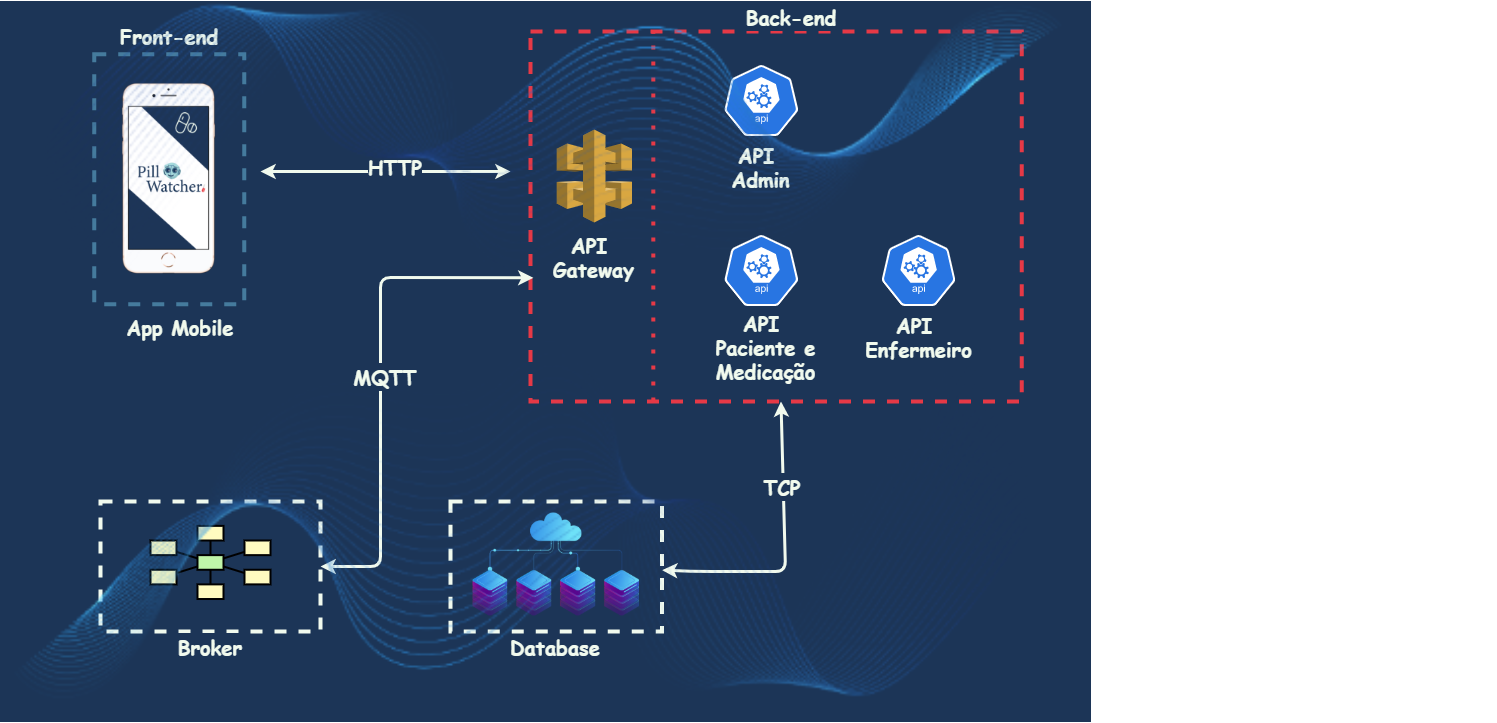
\includegraphics[width=\textwidth]{figuras/software/solucao_software.png}
    \caption{Solução de Software}
    \label{fig:software_solution}
\end{figure}

Assim, o objetivo da solução consiste em estabelecer a comunicação do usuário com o dispositivo através de um dispositivo móvel. Serão utilizados conceitos como Arquitetura de Microsserviços, \emph{Internet of Things}, \emph{Reactive Programming} e \emph{Cloud Deploy}.

\subsection{Banco de Dados}

Para armazenar dados referentes à biometria dos enfermeiros, cadastro de pacientes, administradores e enfermeiros, medicações e receitas médicas, optou-se pela utilização da tecnologia de banco de dados \emph{MySQL}. 

O banco de dados relacional \emph{MySQL} é um conjunto de dados relacionais, estruturados ou organizados na forma de tabelas, colunas e linhas, onde as tabelas representam os objetos, as colunas representam os campos e as linhas representam os registros \cite{EDUCBA_2020}.

Os dados referentes ao cadastro de medicações, pacientes, enfermeiros, entre outros, serão armazenados na nuvem, utilizando os servidores \textit{Linux} da \textit{One Click Hosting}. Por outro lado, dados referentes à biometria do enfermeiro serão armazenados localmente, dentro da aplicação física, gerenciados pelo sistema embarcado explicitado na solução de eletrônica na seção \ref{sec:sistema_embarcado}.

O armazenamento na nuvem é adquirido de um fornecedor externo, no caso da presente solução, o provedor utilizado é o \textit{One Click Hosting}, que opera a capacidade de armazenamento físico de dados. Sendo assim, esses fornecedores de armazenamento na nuvem gerenciam a capacidade, a segurança e a resiliência para disponibilizar dados aos aplicativos em todo o mundo \cite{AMAZONWEBSERVICES_2020}.

\subsection{Back-end}\label{sec:software_backend}
O \emph{Back-end} é a camada onde ocorre o processamento da lógica negocial e é o componente do software que estabelece conexão com a base de dados para registrar e/ou prover informações a um cliente. Dessa forma, tanto a aplicação móvel, quanto ao sistema embarcado instalado no dispensador de remédios se comunicaram com essa camada.

O \emph{Back-end} é desenvolvido a partir da utilização da arquitetura de microsserviços, aplicando o \emph{framework Spring} (\emph{Boot, Data, Security}) e bibliotecas (\emph{libs}) em \textit{Python} para a validação de impressões digitais. Tais aplicações estabelecem comunicação entre si através de um sistema gerenciador (\emph{API Gateway}), utilizando \textit{Spring Cloud}.

Para a integração do \textit{Back-end} com o dispensador de medicamentos, tem-se o emprego dos conceitos de \emph{Internet of Things}. Dessa forma, para o repasse e recebimento de informações será utilizado o \emph{middleware} de filas \textit{Mosquitto}. Logo, as requisições à fila utilizam o protocolo MQTT.

A configuração de ambiente será realizada através da tecnologia \textit{Docker}. Em ambientes de produção, as aplicações serão implantadas nos servidores em nuvem da \textit{One Click Hosting}.

\subsection{Front-end}
A aplicação móvel, desenvolvida utilizando o \emph{framework} \textit{React Native}, proveem uma interface para o gerenciamento dos diversos tipos de usuários (pacientes, enfermeiros e administradores). 

Assim, a aplicação é responsável por facilitar o gerenciamento de receitas médicas de seus pacientes e seus respectivos medicamentos, bem como notificar o enfermeiro(a) quando estiver no horário da medicação e quando o estoque de algum medicamento estiver baixo. A aplicação móvel tem como objetivo facilitar a análise de dados através da geração de gráficos e relatórios necessários aos seus usuários. 

Por último, a aplicação é responsável por validar os medicamentos dispensados pela máquina e após esse procedimento, será exibida uma tela onde o profissional confirmará se a medicação foi ministrada ou não.

\subsection{Broker}

É o elemento responsável por gerir as publicações e as subscrições do protocolo MQTT. Ele é como uma espécie de mediador entre as máquinas. A mensagem é enviada ao \textit{broker}, que é capaz de entender e ler múltiplos aparelhos ao mesmo tempo, através da base de TCP/IP os aparelhos leem as mensagens e aproveitam as que fazem sentido de alguma forma.

% Antes da construção acho que seria importante adicionar um /subsection{Broker}

\section{Plano de Construção e Entrega de Software}
Para efetuar a validação de alterações realizadas em código fonte, optou-se utilizar \textit{Travis CI} para integração contínua, em que são definidas as etapas descritas abaixo:

\begin{itemize}
    \item \emph{Build}: é construído o código-fonte e verificado se o mesmo está de acordo com padrões de Folha de Estilo pré-definidos em \href{https://github.com/PillWatcher/Documentacao/wiki/Folha-de-Estilo}{\emph{Pillwatcher} - Folhas de Estilo};
    \item  \emph{Test}: são realizados os testes unitários e verificados se todos se encontram em estado aprovado;
    \item  \emph{SonarQube Analysis}: o código-fonte é analisado e comparado com métricas de confiabilidade, segurança, manutenibilidade, cobertura de testes e duplicação de código, a partir da execução de revisões automáticas com análise estática do código para detecção de odores de código e vulnerabilidades de segurança;
    \item  \emph{Deploy}: a solução é implantada em um ambiente de produção e/ou desenvolvimento. 
\end{itemize}

%O \textit{SonarQube} conforme descrito na etapa \textit{SonarQube Analysis}, trata-se de uma ferramenta em código aberto desenvolvida pela empresa \textit{SonarSource} para inspeção contínua da qualidade do código, execução de revisões automáticas com análise estática do código para detecção de odores de código e vulnerabilidades de segurança em mais de 20 linguagens de programação.

Dessa forma, com o objetivo de entregar um código testado e livre de inconsistências, optou-se pela utilização do conceito TDD (\emph{Test Driven Development}), o qual consiste no desenvolvimento de testes unitários antes do desenvolvimento de funcionalidades. Optou-se também pela metodologia de desenvolvimento orientado à métricas, as quais o \textit{SonarQube} mede e valida.

\begin{figure}[H]
    \centering
    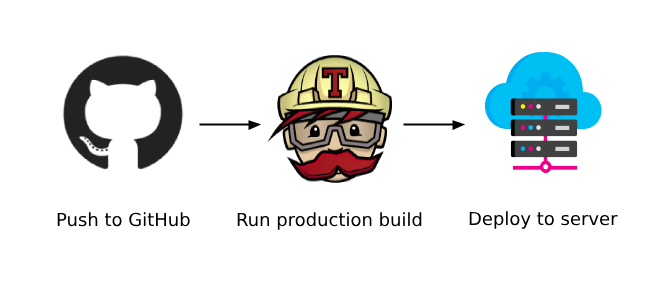
\includegraphics[width=1.0\textwidth]{figuras/software/deploy-continuous.png}
    \caption{Software \textit{Deploy}}
    \label{fig:software_deploy}
\end{figure}

A etapa de \emph{Deploy}, listada acima e ilustrada pela Fig. \ref{fig:software_deploy}, depende de um ambiente pré-configurado para ser realizada. Para isso, optou-se por utilizar o \textit{Docker} para conteinerização de softwares auxiliares e a \textit{One Click Hosting} para hospedagem dos serviços em nuvem.

\section{Nonfunctional Requirements (NFRs) }

Os Requisitos Não Funcionais (NFRs) definem os atributos do sistema, como: segurança, confiabilidade, desempenho, escalabilidade e usabilidade. Eles servem como restrições ao design do sistema entre os diferentes acúmulos.

Também conhecidos como qualidades do sistema, os requisitos não funcionais são tão críticos quanto as epopeias, recursos e histórias funcionais. Eles garantem a usabilidade e eficácia de todo o sistema. O não cumprimento de qualquer um deles pode resultar em sistemas que não atendem às necessidades internas do negócio, do usuário ou do mercado.

% Até esse ponto são definições, temos que ver com o Chaim se devemos manter, mas acho que seria interessante explicar como esse conceito é aplicado no produto.

Um aspecto importante em uma solução de software é a confiabilidade representada na Fig. \ref{fig:nfr-confiabilidade}. Para atingir essa meta, foram levantadas três condições que precisam ser atendidas para essa característica ser cumprida, são elas: proteção de dados dos usuários, autenticação de contas e limitação no cadastro. Para alcançar a primeira, será utilizada a tecnologia \textit{Spring Security} que assegurará os dados dos usuários. A segunda será satisfeita por meio da utilização de biometria e de login por CPF e senha. Por último, a solução atua em um cenário sensível, assim é necessário garantir uma limitação no cadastro que será totalizada quando o administrador for inserido na aplicação, esse irá cadastrar os enfermeiros, os quais, por conseguinte, serão os responsáveis pelo cadastro dos pacientes. 

\begin{figure}[H]
    \centering
    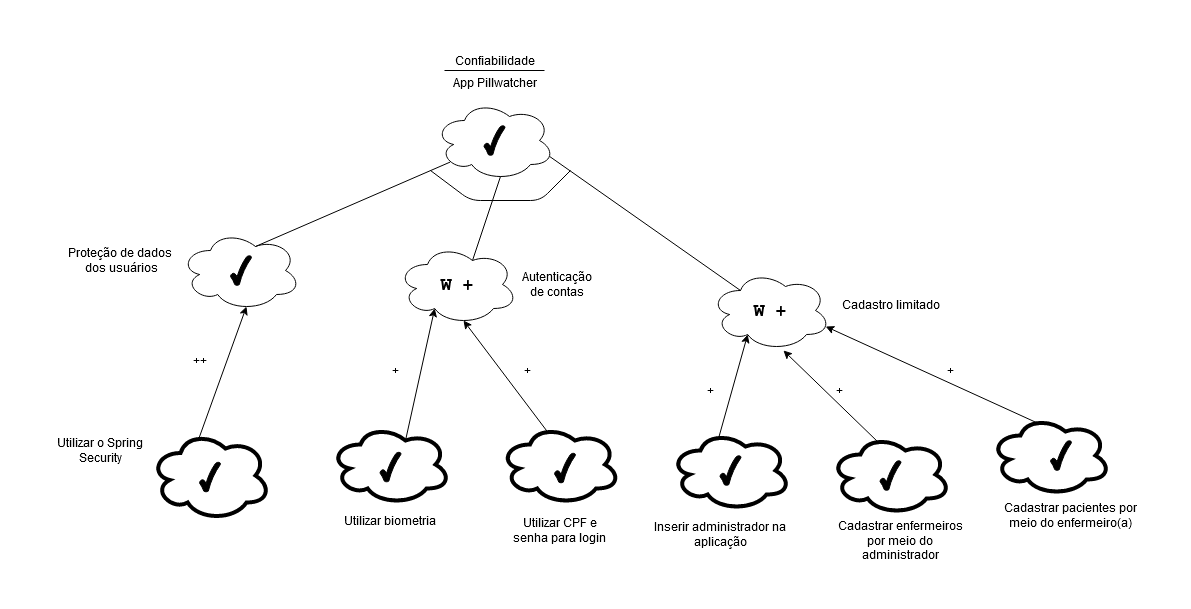
\includegraphics[width=16cm, height=16cm, keepaspectratio]{figuras/software/NFR/NFR_confiabilidade.png}
    \caption{NFR de confiabilidade}
    \label{fig:nfr-confiabilidade}
\end{figure}

Outro aspecto extremamente importante para o desenvolvimento de um software seguro é assegurar que os pilares autenticidade, confidencialidade e integridade estejam presentes conforme apresentado na Fig. \ref{fig:nfr-seguranca}. Para garantir a autenticidade do sistema será implementado um sistema de autenticação, que será feito em duas partes, uma com a autenticação no aplicativo e outra via biometria, essa última feita diretamente na máquina. Para que o pilar da confidencialidade seja satisfeito, será aplicado ao sistema o gerenciamento de acessos que dará permissões restritas a depender do tipo de usuário cadastrado. O pilar de integridade do sistema depende da verificação e execução dos testes de software como por exemplo os testes unitários.

\begin{figure}[H]
    \centering
    \includegraphics[width=15cm, height=15cm, keepaspectratio]{figuras/software/NFR/NFR_segurança.png}
    \caption{NFR de segurança}
    \label{fig:nfr-seguranca}
\end{figure}

Com relação aos aspectos que afetam o desempenho da aplicação como na Fig \ref{fig:nfr-desempenho}, tem-se a redução do uso de memória por meio de uma dinâmica de páginas que limitam o volume de informações apresentadas diretamente em tela. A melhoria do \emph{design} será garantido por meio da aplicação de um \emph{design} minimalista e a redução da utilização de recursos do servidor e otimização do tempo de resposta por meio da hospedagem de um servidor eficiente como o \textit{Heroku}.

\begin{figure}[H]
    \centering
    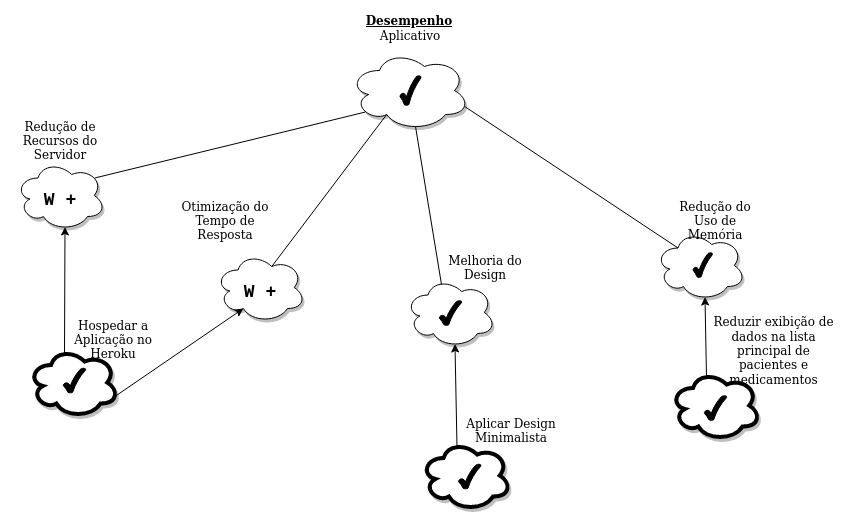
\includegraphics[width=15cm, height=15cm, keepaspectratio]{figuras/software/NFR/NFR_desempenho.png}
    \caption{NFR de desempenho}
    \label{fig:nfr-desempenho}
\end{figure}

Para atender aos módulos de usabilidade da aplicação e consequentemente atender as necessidades de utilização do usuário como Fig. \ref{fig:nfr-usabilidade}, tem-se um enfoque em três pontos principais: boa comunicação via mensagens significativas e de boa compreensão do usuário, implementação de uma interface simples por meio de uma boa organização de elementos, bem como a consistência e padronização dos componentes. Outro ponto é a facilidade de utilização que exija uma curva de aprendizado menor do usuário em relação a utilização da aplicação por meio de um \textit{design} intuitivo.

\begin{figure}[H]
    \centering
    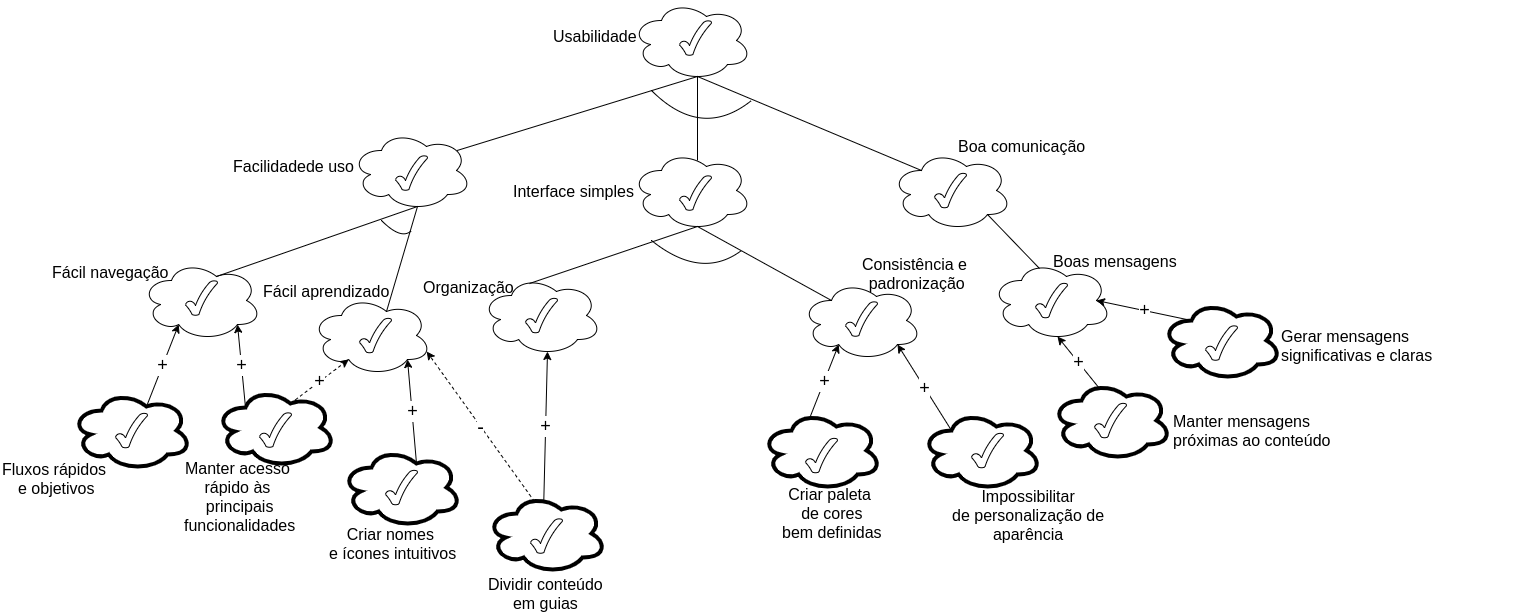
\includegraphics[width=14cm, height=18cm, keepaspectratio]{figuras/software/NFR/NFR_usabilidade.png}
    \caption{NFR de usabilidade}
    \label{fig:nfr-usabilidade}
\end{figure}

%\section{Arquitetura da Informação}
\section{Modelo Entidade Relacionamento - MER}

O Modelo Entidade Relacionamento (também chamado Modelo ER, ou simplesmente MER), como o nome sugere, é um modelo conceitual utilizado na Engenharia de \textit{Software} para descrever os objetos (entidades) envolvidos em um domínio de negócios, com suas características (atributos) e como elas se relacionam entre si (relacionamentos) \cite{DEVMEDIA_2014}.

O MER abaixo representa as entidades necessárias para desenvolver o aplicativo \emph{PillWatcher}. Dessa forma, foi utilizado o idioma Inglês para descrever as entidades e seus atributos. A modelagem está na quarta forma normal, assim atendendo as principais regras de qualidade de banco de dados.

\begin{figure}[H]
    \centering
    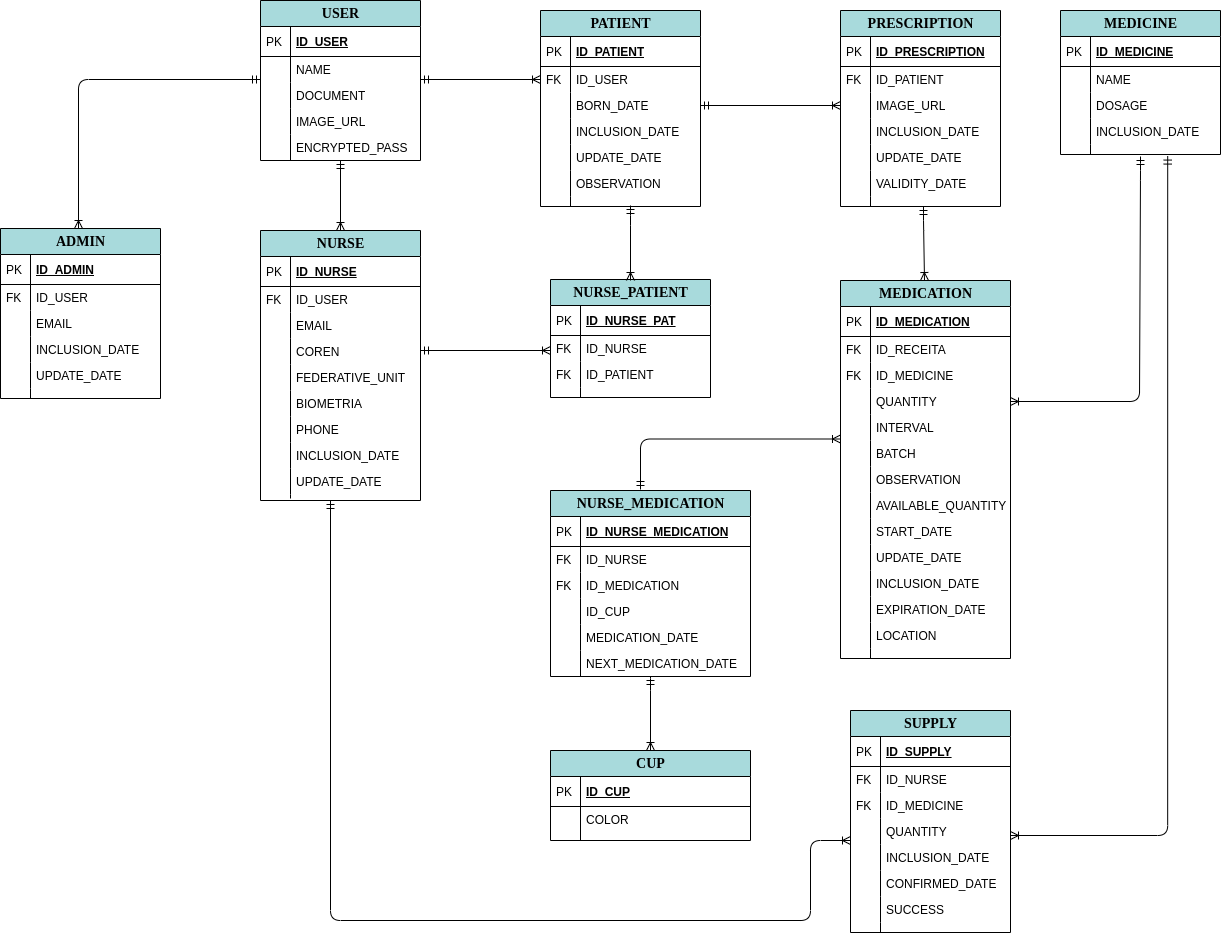
\includegraphics[width=0.9\textwidth]{figuras/software/database.png}
    \caption{MER}
    \label{fig:der}
\end{figure}

Para melhor entendimento, seguem breves explicações de cada entidade:

\begin{itemize}
    \item[]
\begin{enumerate}
  \item \emph{USER}: um usuário generalizado.
  \item \emph{ADMIN}: especialização de \emph{User}, representa o administrador do sistema.
  \item \emph{NURSE}: especialização de \emph{User}, representa o enfermeiro do sistema.
  \item \emph{PATIENT}: especialização de \emph{User}, representa o paciente do sistema.
  \item \emph{NURSE PATIENT}: associação entre paciente e enfermeiro. Pois um enfermeiro pode cuidar de vários pacientes, e um paciente pode ser observado por vários enfermeiros.
  \item \emph{PRESCRIPTION}: receita médica de um paciente.
  \item \emph{MEDICATION}: medicação que compõe uma receita.
  \item \emph{MEDICINE}: remédio disponível no dispensador e que compõe uma medicação.
  \item \emph{NURSE MEDICATION}: associação entre enfermeiro e medicação. Pois uma medicação ao paciente é gerida por um enfermeiro.
  \item \emph{CUP}: copo para medicação ao paciente.
  \item \emph{SUPPLY}: abastecimento feito no dispensador por um enfermeiro.
\end{enumerate}
\end{itemize}

\section{Diagramas UML}

Os diagramas UML podem ajudar arquitetos e desenvolvedores de sistema a entender, colaborar e desenvolver um aplicativo. Arquitetos e gerenciadores de alto nível podem usar diagramas UML para visualizar todo o sistema ou projeto e separar aplicativos em componentes menores para desenvolvimento \cite{IBM}.

Existem diferentes tipos de diagramas UML, e para o projeto foram escolhidos os de caso de uso, pacotes e sequência. Juntos, eles trazem uma visão dos requisitos do sistema, arquitetura interna do \emph{back-end} e também uma visão geral das atividades.

\subsection{Diagramas de Caso de Uso}

Os diagramas de casos de uso descrevem as funções principais de um sistema e identificam as interações entre o sistema e seu ambiente externo, representado por agentes. Esses agentes podem ser pessoas, organizações, máquinas ou outros sistemas externos \cite{IBM}. Abaixo tem os diagramas separados dos principais usuários do sistema.

\begin{enumerate}
    \item Diagrama de Caso de Uso do Mantenedor
    
\begin{figure}[H]
    \centering
    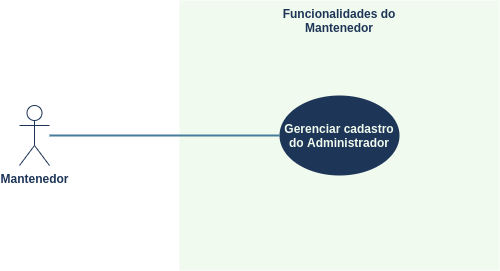
\includegraphics[width=0.5\textwidth]{figuras/software/UML/matenedor-us.png}
    \caption{Diagrama de Caso de Uso - Mantenedor}
    \label{fig:mantenedor_us}
\end{figure}

Nesse diagrama, foi listada a principal e única funcionalidade do usuário mantenedor, a qual consiste em gerenciar cadastro do administrador.

    \item Diagrama de Caso de Uso do Sistema
    
\begin{figure}[H]
    \centering
    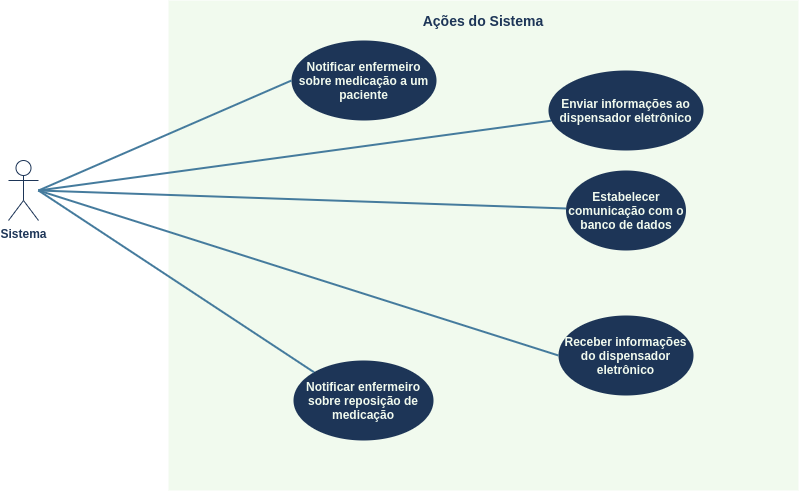
\includegraphics[width=0.5\textwidth]{figuras/software/UML/sistema-us.png}
    \caption{Diagrama de Caso de Uso - Sistema}
    \label{fig:sistema_us}
\end{figure}

Nesse digrama foram listadas as principais ações do sistema. O diagrama de caso de uso do sistema executa diversas ações isoladamente que são de extrema importância para o fluxo do projeto \emph{PillWatcher}, como exemplo notificar o enfermeiro de ações que ele deve tomar.

    \item Diagrama de Caso de Uso do Enfermeiro
    
\begin{figure}[H]
    \centering
    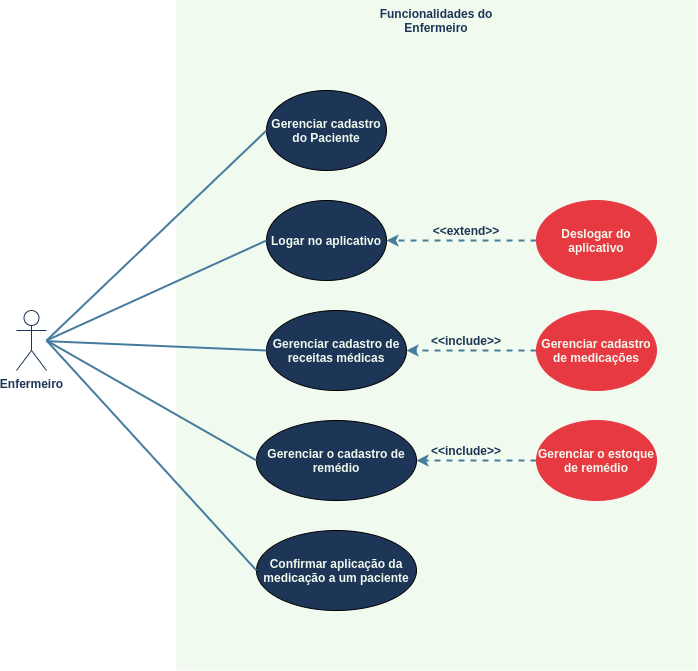
\includegraphics[width=0.5\textwidth]{figuras/software/UML/enfermeiro-us.png}
    \caption{Caso de Uso - Enfermeiro}
    \label{fig:enfermeiro_us}
\end{figure}

Nesse digrama, foram listadas as principais funcionalidades do enfermeiro, o qual é o usuário principal do sistema.

    \item Diagrama de Caso de Uso do Administrador

\begin{figure}[H]
    \centering
    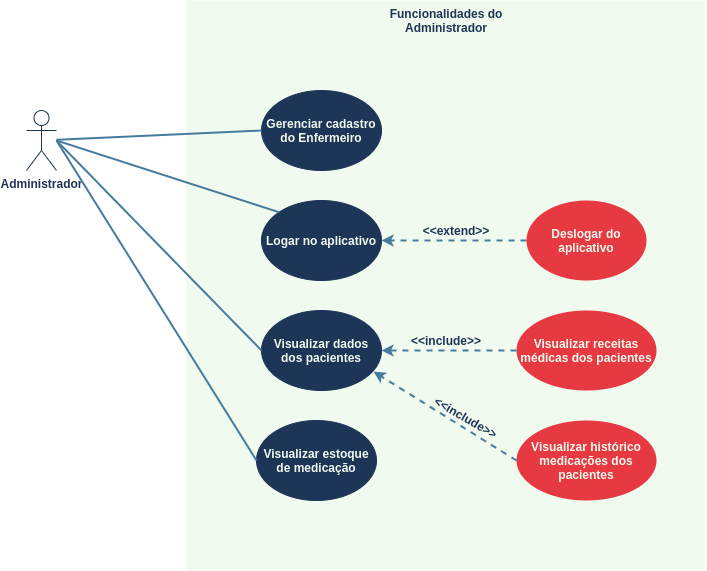
\includegraphics[width=0.6\textwidth]{figuras/software/UML/administrador-us.png}
    \caption{Caso de Uso - Administrador}
    \label{fig:administrador_us}
\end{figure}

Nesse digrama, foram listadas as principais funcionalidades do administrador. Esse usuário apenas gerencia o cadastro do enfermeiro e visualiza todos os dados disponíveis no aplicativo.

\end{enumerate}

\subsection{Diagrama de Pacotes}

Os Diagramas de pacotes são módulos do sistema divididos em agrupamentos lógicos mostrando a dependência entre eles.
Foi diagramado os pacotes que fazem parte da solução \emph{back-end}, como mostra a figura abaixo:

\begin{figure}[H]
    \centering
    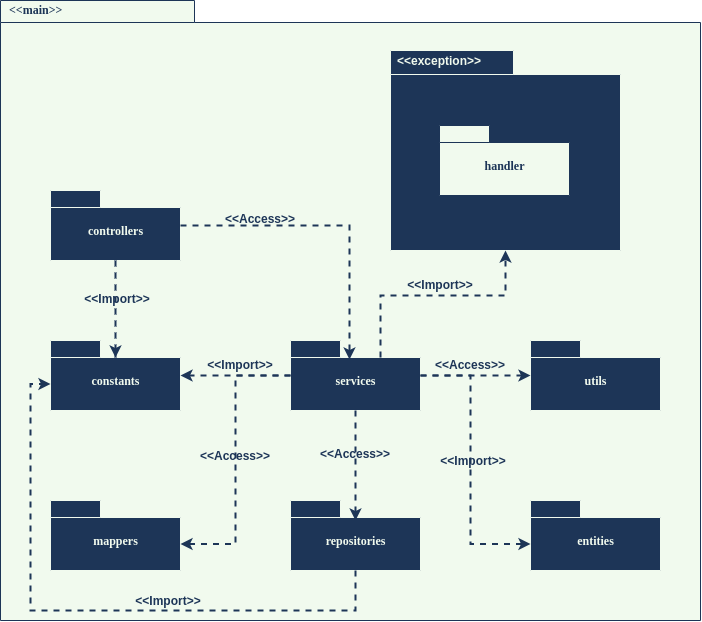
\includegraphics[width=0.9\textwidth]{figuras/software/diagrama-pacote.png}
    \caption{Diagrama de Pacotes do \emph{Back-end}}
    \label{fig:pacotes-diagrama}
\end{figure}

Assim, cada pacote ilustrado tem um papel específico dentro do projeto, e estão descritos abaixo:

\begin{itemize}
\item[]
    \begin{enumerate}
      \item \textit{Controllers}: possui todas as classes que se comunicam com o mundo externo por meio de requisições HTTP.
      \item \textit{Constants}: possui classes/interfaces com atributos contantes utilizados em todo o projeto.
      \item \textit{Services}: possui classes/interfaces que implementam a lógica negocial.
      \item \textit{Mappers}: possui interfaces que transformam um objeto em outro.
      \item \textit{Repositories}: possui interfaces que se comunicam com o banco de dados.
      \item \textit{Entities}: possui classes que são representações de entidades no banco de dados.
      \item \textit{Utils}: possui classes utilitárias, usadas por todo o projeto.
      \item \textit{Exceptions}: possui classes que definem todas as exceções geradas no projeto.
      \item \textit{Handler}: possui classes que tratam as exceções geradas no projeto.
    \end{enumerate}
\end{itemize}

\section{Arquitetura da Informação}

\subsection{Identidade Visual}
As definições acerca da identidade visual do \emph{Pillwatcher} estão disponíveis em \href{https://github.com/PillWatcher/Documentacao/wiki/Identidade-Visual}{\emph{Pillwatcher} - Identidade Visual} e \href{https://github.com/PillWatcher/Documentacao/wiki/Logomarca}{\emph{Pillwatcher} - Logomarca}

\subsection{Protótipo de Alta Fidelidade}
A prototipagem de alta fidelidade é a técnica que mais se aproxima do produto final. Por meio da aplicação dessa, é possível avaliar questões de Interface do Usuário (\emph{UI -  User Interface}) e de Experiência do Usuário \emph{(UX - User Experience)}. Sendo esses conteúdos extremamente relevantes em termos de desenvolvimento de \textit{front-end}. O protótipo desenvolvido na ferramenta Figma está disponível em \href{https://www.figma.com/proto/60dT2EKBbcIPKy5Tg0Zzpg/App_Pillwatcher?node-id=1\%3A5\&scaling=scale-down}{Protótipo do \emph{App Pillwatcher}} e abaixo esse está ilustrado divido por fluxos.  

% \subsubsection*{Login}
\subparagraph*{$\bullet$ Login} \hfill

A tela na Fig. \ref{fig:prototipo_tela_inicial_e_login}, apresenta as telas iniciais da aplicação. Esta é uma tela que será exibida logo após a inicialização da aplicação móvel e é responsável por autenticar os usuários na aplicação. 

\begin{figure}[H]
    \centering
    \subfloat[][Tela inicial e Tela de Login]{
    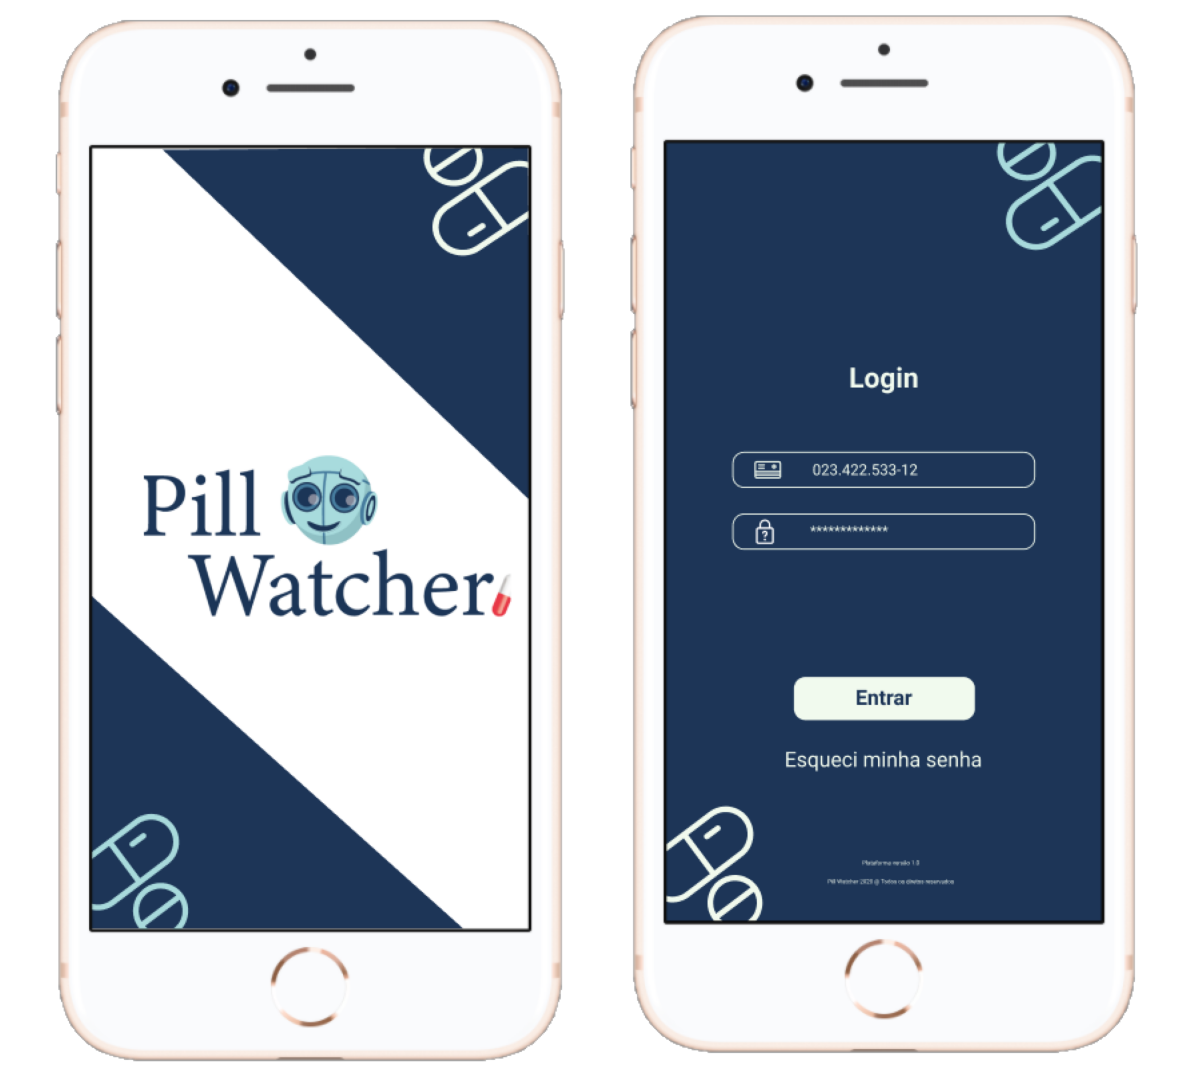
\includegraphics[width=8cm]{figuras/software/Atual_prototipo/Login_1.png}
    \label{fig:prototipo_tela_inicial_e_login}}
    \subfloat[][Fluxo de recuperar senha]{
    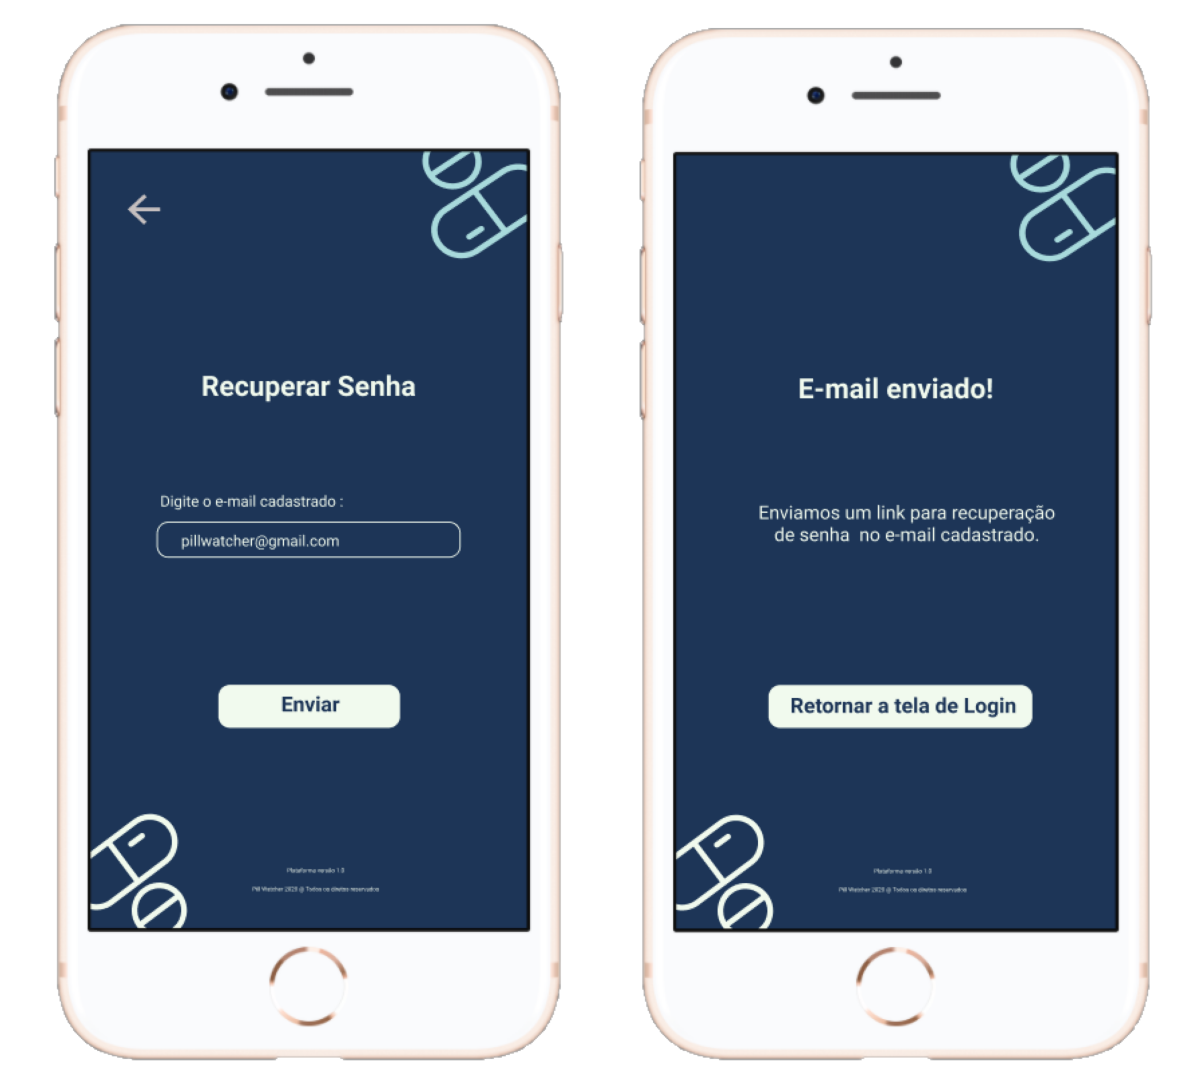
\includegraphics[width=8cm]{figuras/software/Atual_prototipo/Login_2.png}
    \label{fig:prototipo_fluxo_recuperar_senha}}
    \caption{Login}
\end{figure}

A Fig. \ref{fig:prototipo_fluxo_recuperar_senha} retrata o fluxo de recuperação de senha que auxiliará o usuário na ação de alterar a senha antiga para uma nova senha e assim permitir novamente seu acesso à aplicação.


\begin{table}[H]
    \centering
    \caption{Tabela de Interações das Telas Iniciais do Aplicativo}
    \label{tab:interacao-telas-inicias}
    \begin{adjustbox}{max width = \textwidth}
    % \begin{adjustwidth}{-2,5cm}{}
        \begin{tabular}{|L{5cm}|L{4cm}|L{6cm}|L{4cm}|L{4cm}|}
            \hline
            \rowcolor[HTML]{A8DADC}
            \multicolumn{1}{|c|}{\textbf{Tela}} & \multicolumn{1}{c|}{\textbf{Entrada}} & \multicolumn{1}{c|}{\textbf{Interações}} & \multicolumn{1}{c|}{\textbf{Saída}} & \multicolumn{1}{c|}{\textbf{Alternativo}}\\ \hline
             Tela Inicial & Abrindo o aplicativo & \multicolumn{1}{c|}{---} & Tela de Login & \multicolumn{1}{c|}{---} \\ \hline
             Tela de Login & Após carregamento & Digitar CPF e senha, clicar no botão de recuperar senha & Tela de opções  & O caminho alternativo seria o usuário ser direcionado para a Tela de recuperar senha \\ \hline
             Tela de recuperar senha & Usuário clicar no botão de recuperar senha & Digitar o \textit{e-mail} cadastrado e clicar no botão enviar & Modal de envio do link de recuperação de senha & \multicolumn{1}{c|}{---} \\ \hline
             
             Modal de envio do link de recuperação de senha & Usuário clicar no botão enviar & Clicar no botão de retornar para a tela de login  & Tela de Login & \multicolumn{1}{c|}{---} \\ \hline
             
        \end{tabular}
    % \end{adjustwidth}
    \end{adjustbox}
\end{table}

% \subsubsection{Administrador(a)}
\subparagraph*{$\bullet$ Administrador(a)} \hfill
% \subsubsubsection{Menu Inicial do Administrador}
\subparagraph*{} $-$ Menu Inicial do Administrador

A Fig. \ref{fig:prototipo_admin_tela_inicial_e_sidebar} apresenta as opções de execução de gerenciamento que o usuário administrador possui permissão dentro da aplicação. Na imagem à direta exibe-se os dados pessoais do usuário administrador na \textit{sidebar} da aplicação, bem como sua permissão para edição de dados do perfil e saída da aplicação.

\begin{figure}[H]
    \centering
    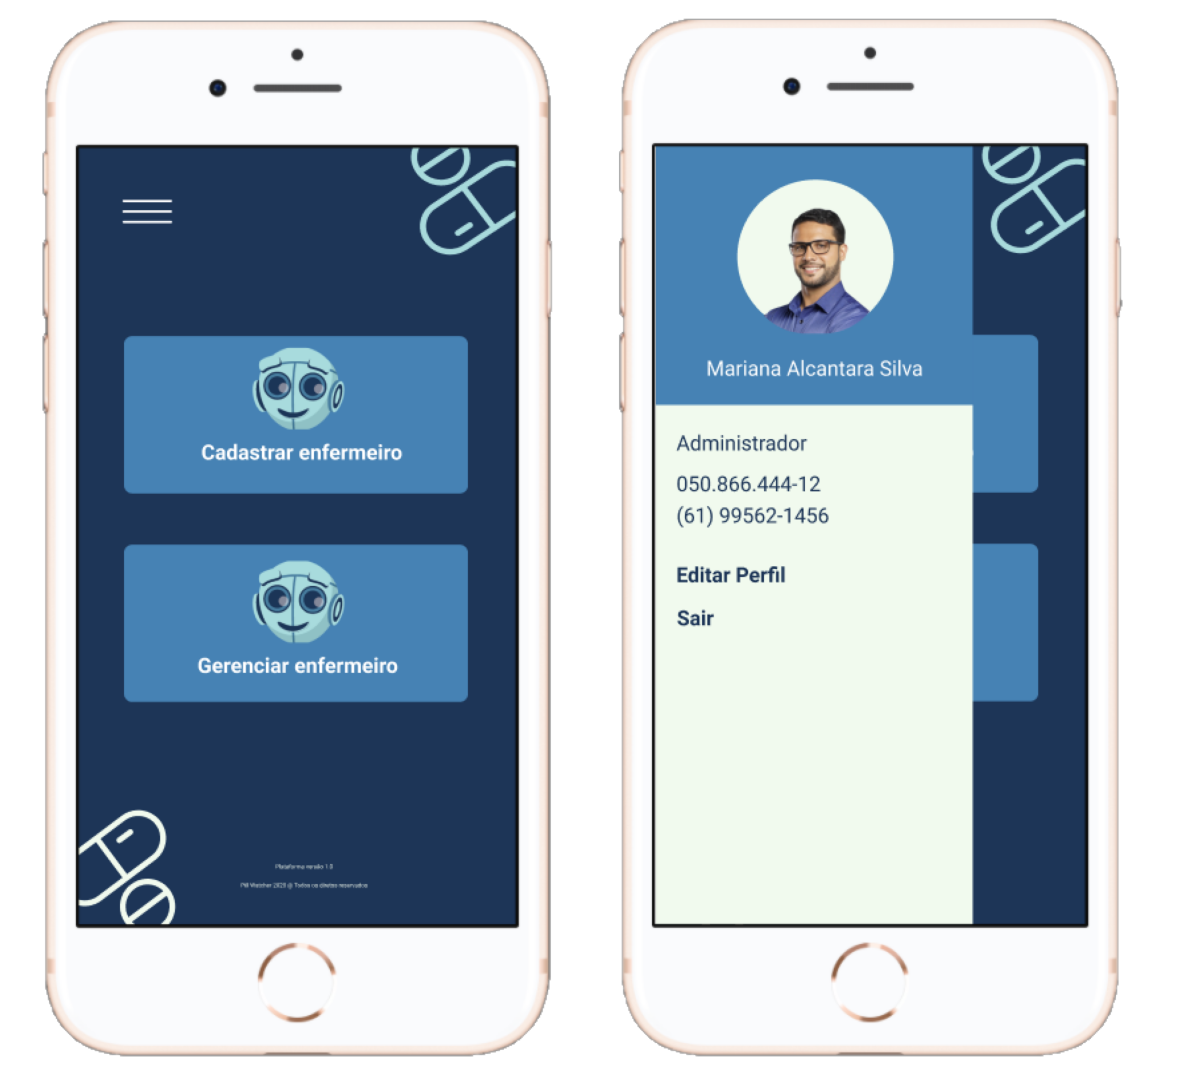
\includegraphics[width=12cm]{figuras/software/Atual_prototipo/Admin_TelaInicial_e_Sidebar.png}
    \caption{Administrador - Menu Inicial}
    \label{fig:prototipo_admin_tela_inicial_e_sidebar}
\end{figure}

Na sequencia, a Fig. \ref{fig:prototipo_admin_alterarDados} representa a tela de edição de perfil que permitirá ao usuário administrador, alterar seus dados pessoais cadastrados na aplicação, bem como adicionar uma nova foto de perfil e receber um \textit{feedback} com relação ao sucesso na execução da alteração de dados na aplicação.

\begin{figure}[H]
    \centering
    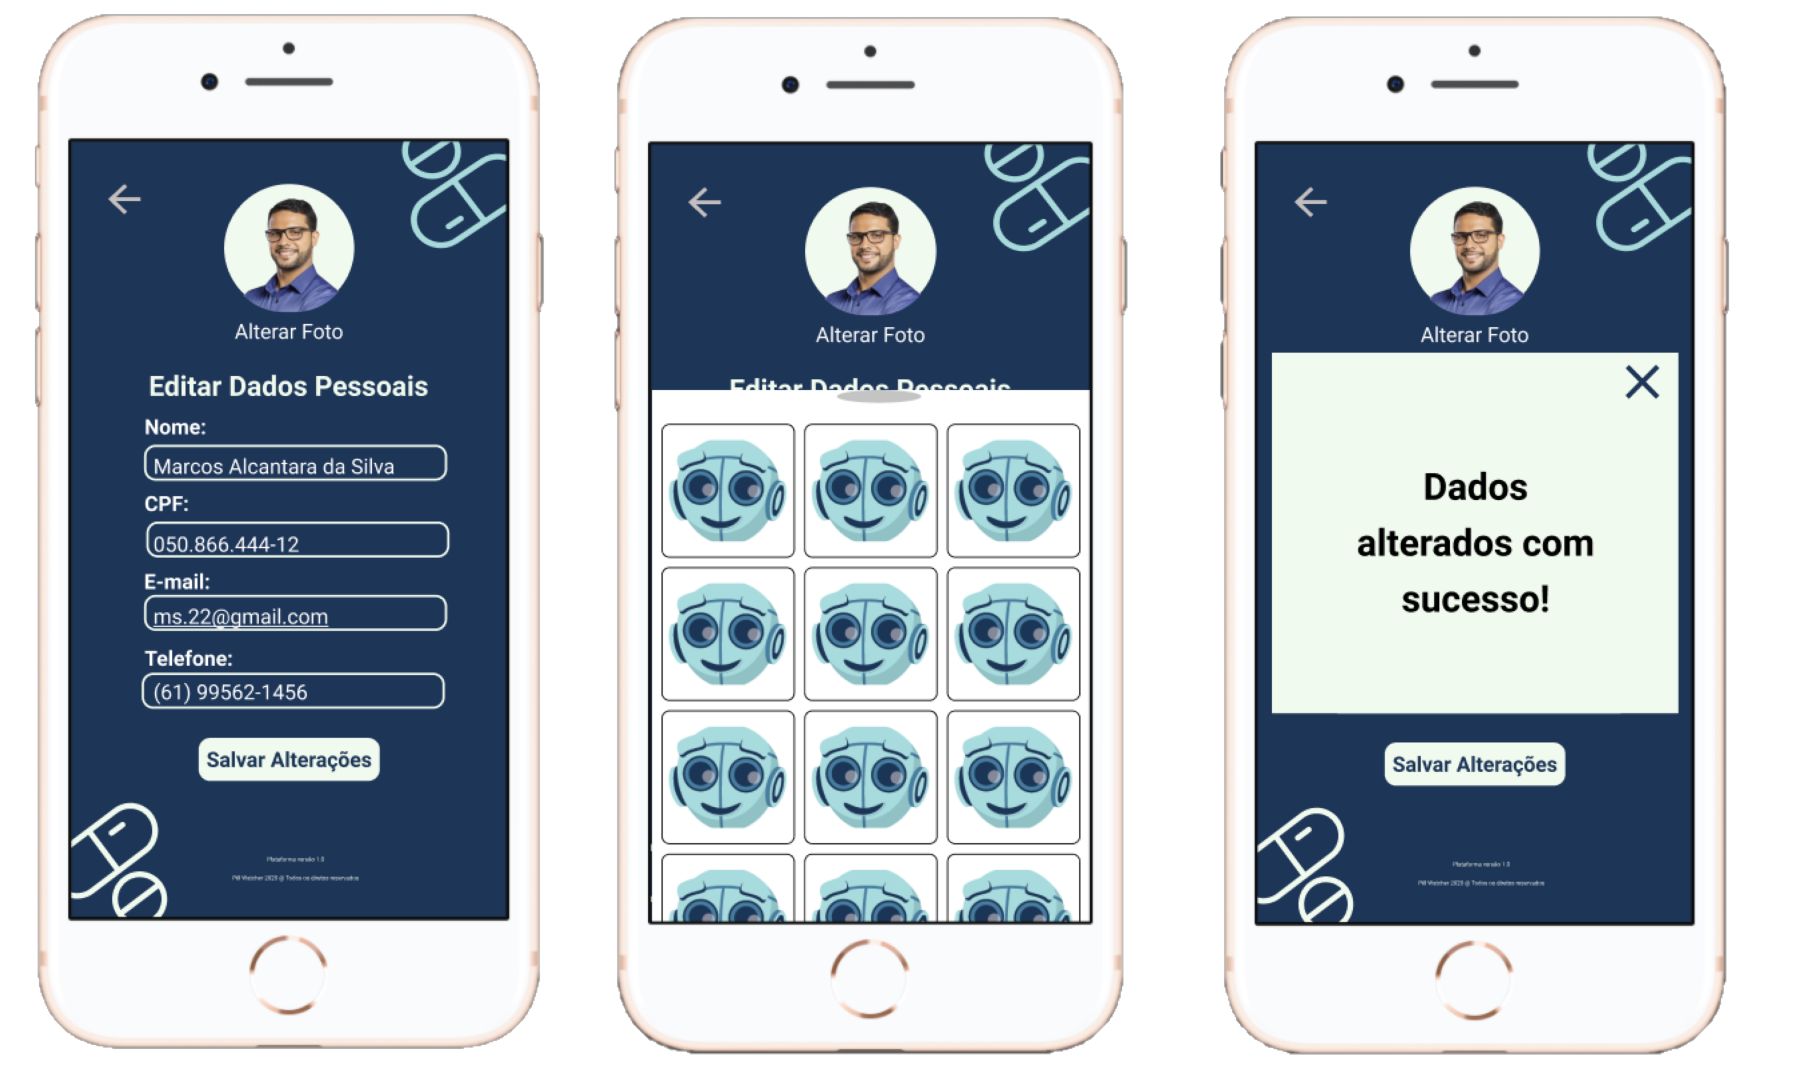
\includegraphics[width=15cm]{figuras/software/Atual_prototipo/Admin_AlterarDados.png}
    \caption{Administrador - Fluxo de alteração de dados}
    \label{fig:prototipo_admin_alterarDados}
\end{figure}

\begin{table}[H]
    \centering
    \caption{Tabela de Interações das Telas Principais de Administrador}
    \label{tab:interacao-telas-adm}
    \begin{adjustbox}{max width = \textwidth}
    % \begin{adjustwidth}{-2,5cm}{}
        \begin{tabular}{|L{5cm}|L{4cm}|L{6cm}|L{4cm}|L{4cm}|}
            \hline
            \rowcolor[HTML]{A8DADC}
            \multicolumn{1}{|c|}{\textbf{Tela}} & \multicolumn{1}{c|}{\textbf{Entrada}} & \multicolumn{1}{c|}{\textbf{Interações}} & \multicolumn{1}{c|}{\textbf{Saída}} & \multicolumn{1}{c|}{\textbf{Alternativo}} \\ \hline
             Tela Principal - Administrador & Realizando o \textit{`Login'} na aplicação & Clicar no botão de acesso a \textit{sidebar}, clicar nos botões de acesso as ações principais do administrador & \multicolumn{1}{c|}{---}  & \multicolumn{1}{c|}{---} \\ \hline
             \textit{Sidebar} - Administrador & Acessando o Menu superior esquerdo da Tela Principal do Administrador & Clicar na opção de edição de dados pessoais, clicar na opção de sair  & \multicolumn{1}{c|}{---} & \multicolumn{1}{c|}{---} \\ \hline
             Tela de Editar Dados Pessoais & Usuário clicar no botão de editar dados & Alterar dados de cadastro & \multicolumn{1}{c|} {Botão Salvar} & \multicolumn{1}{c|}{---} \\ \hline
        \end{tabular}
    % \end{adjustwidth}
    \end{adjustbox}
\end{table}


% \subsubsubsection{Cadastrar enfermeiro}
\subparagraph*{} $-$ Cadastrar enfermeiro

Na Fig. \ref{fig:prototipo_admin_cadastroEnfermeiro_Parte1} é representado a tela de cadastro de enfermeiros que permitirá ao usuário administrador registrar um novo enfermeiro na aplicação, de forma a receber uma orientação na tela seguinte, é retratado a etapa 2 de cadastro de enfermeiro que solicita que o usuário se dirija até a máquina para registrar sua identidade biométrica e assim finalizar o cadastro para que na tela seguinte receba um \textit{feedback} com relação a conclusão do cadastro por meio da identificação do registro biométrico.
\begin{figure}[H]
    \centering
    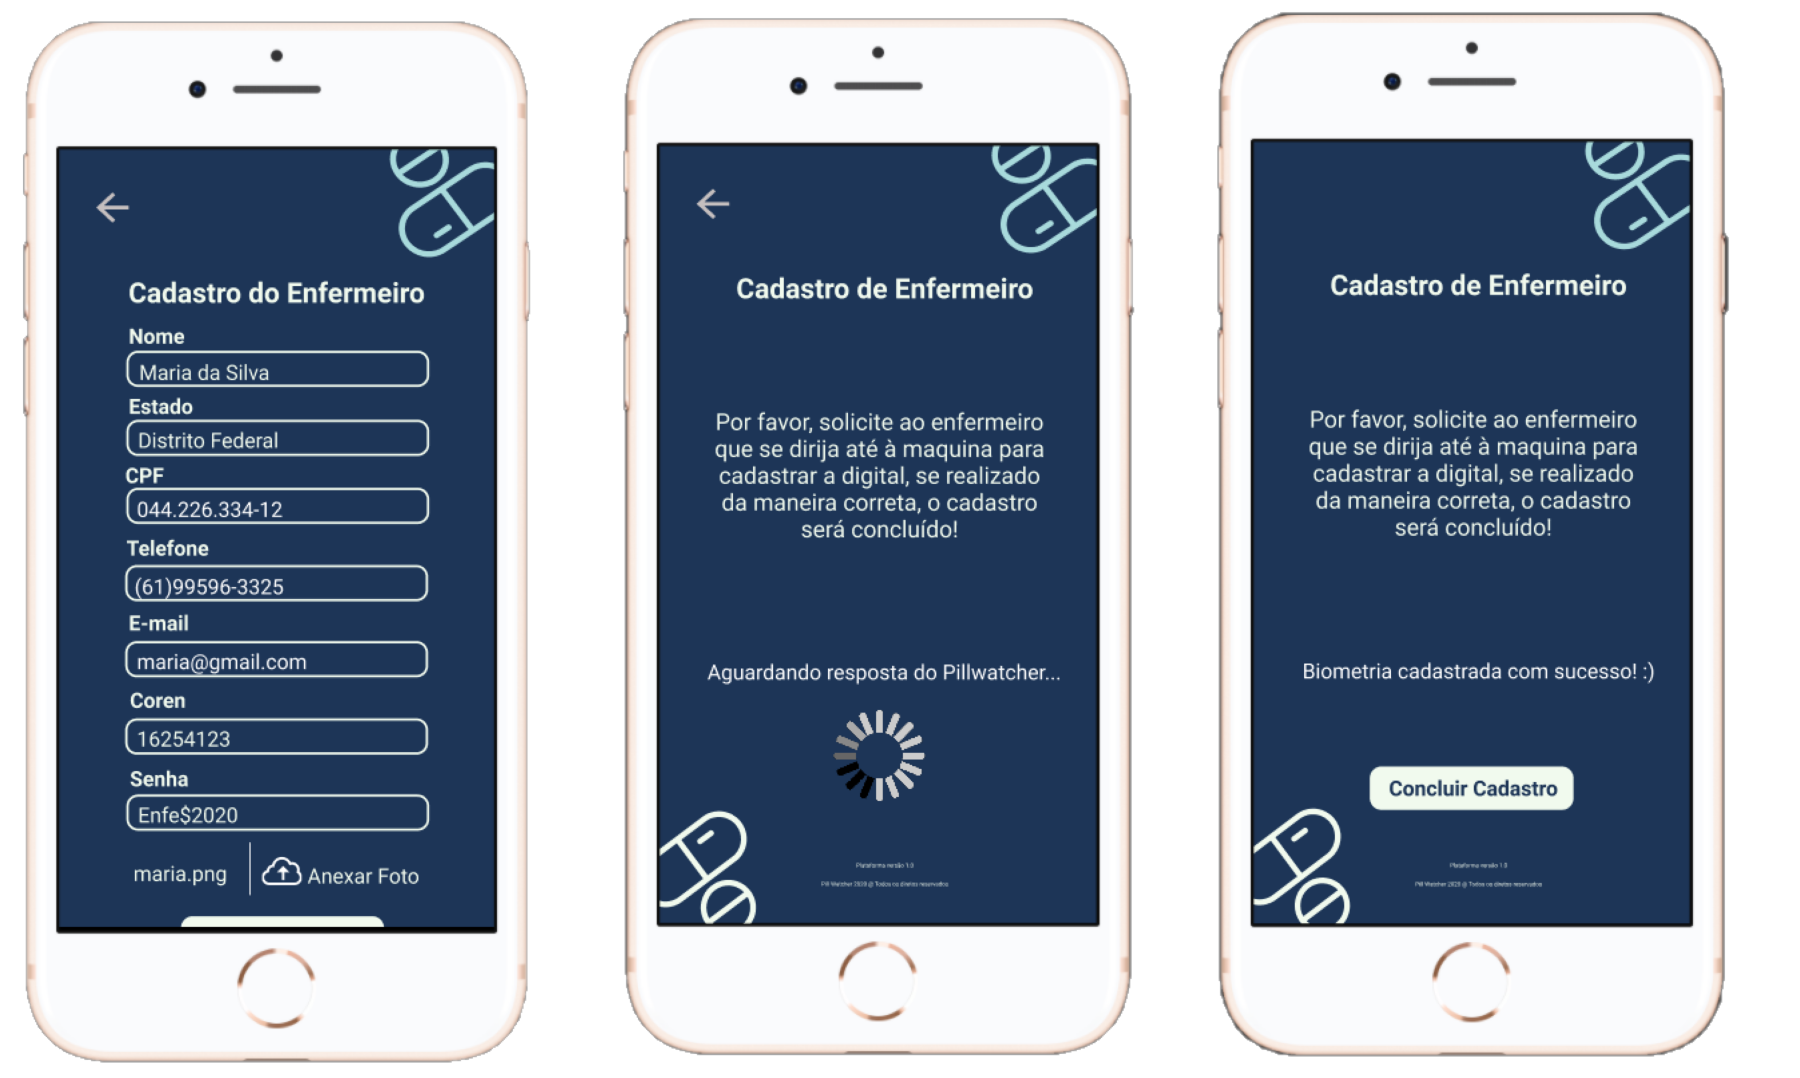
\includegraphics[width=15cm]{figuras/software/Atual_prototipo/Admin_CadastroEnfermeiro.png}
    \caption{Administrador - Fluxo de cadastro de um enfermeiro}
    \label{fig:prototipo_admin_cadastroEnfermeiro_Parte1}
\end{figure}

\begin{table}[H]
    \centering
    \caption{Tabela de Interações das Telas de Cadastro de Enfermeiro}
    \label{tab:interacao-telas-enfermeiro}
    \begin{adjustbox}{max width = \textwidth}
    % \begin{adjustwidth}{-2,5cm}{}
        \begin{tabular}{|L{5cm}|L{4cm}|L{6cm}|L{4cm}|L{4cm}|}
            \hline
            \rowcolor[HTML]{A8DADC}
            \multicolumn{1}{|c|}{\textbf{Tela}} & \multicolumn{1}{|c|}{\textbf{Entrada}} & \multicolumn{1}{|c|}{\textbf{Interações}} & \multicolumn{1}{|c|}{\textbf{Saída}} & \multicolumn{1}{|c|}{\textbf{Alternativo}} \\ \hline
             Tela de Cadastro do Enfermeiro & Botão de Cadastrar Enfermeiro da tela principal & Adicionar nome, estado, CPF, telefone, \textit{e-mail}, \textit{coren}, senha e uma foto de perfil & Icone de Retornar  & \multicolumn{1}{c|}{---} \\ \hline
             Tela de Identificação de Cadastro de Digital do Enfermeiro & Botão 'Cadastrar' & \multicolumn{1}{c|}{---}  & \multicolumn{1}{c|}{---} & \multicolumn{1}{c|}{---} \\ \hline
             Tela de Confirmação de Cadastro & Aguardar confirmação da Tela Anterior & \multicolumn{1}{c|}{---} & Botão Concluir Cadastro & \multicolumn{1}{c|}{---} \\ \hline
        \end{tabular}
    % \end{adjustwidth}
    \end{adjustbox}
\end{table}


% \subsubsubsection{Gerenciar enfermeiros}
\subparagraph*{} $-$ Gerenciar enfermeiros

A Fig. \ref{fig:prototipo_admin_deletarEnfermeiro} e Fig. \ref{fig:prototipo_admin_alterarDados_1} representam o fluxo de gerenciamento do cadastro de enfermeiros na aplicação, no qual permitirá ao usuário administrador editar e/ou excluir um cadastro existente e receber um \textit{feedback} sobre as ações executadas.

\begin{figure}[H]
    \centering
    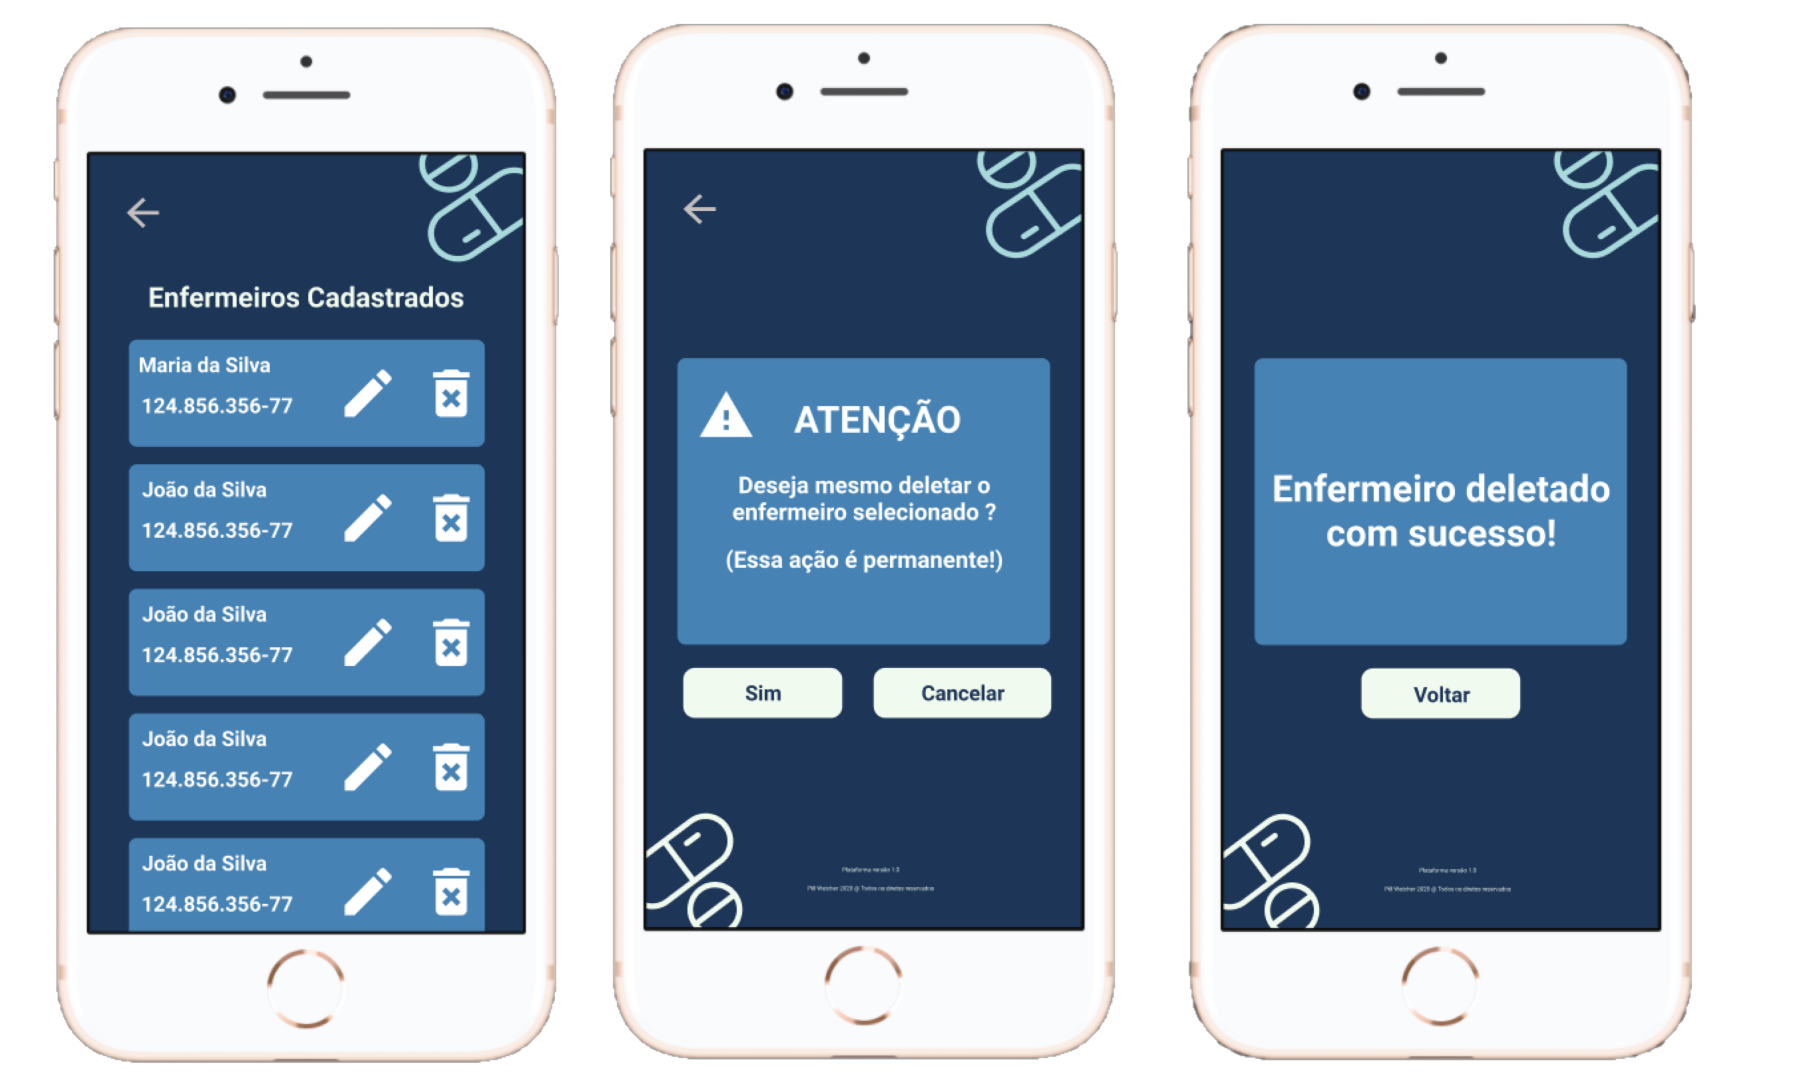
\includegraphics[width=15cm]{figuras/software/Atual_prototipo/Admin_deletarEnfermeiro.png}
    \caption{Administrador - Tela inicial de gerenciar enfermeiros e fluxo para deletar um enfermeiro}
    \label{fig:prototipo_admin_deletarEnfermeiro}
\end{figure}

\begin{figure}[H]
    \centering
    \subfloat[][Tela para alterar dados e \emph{Pop-Up} para alterar foto]{
    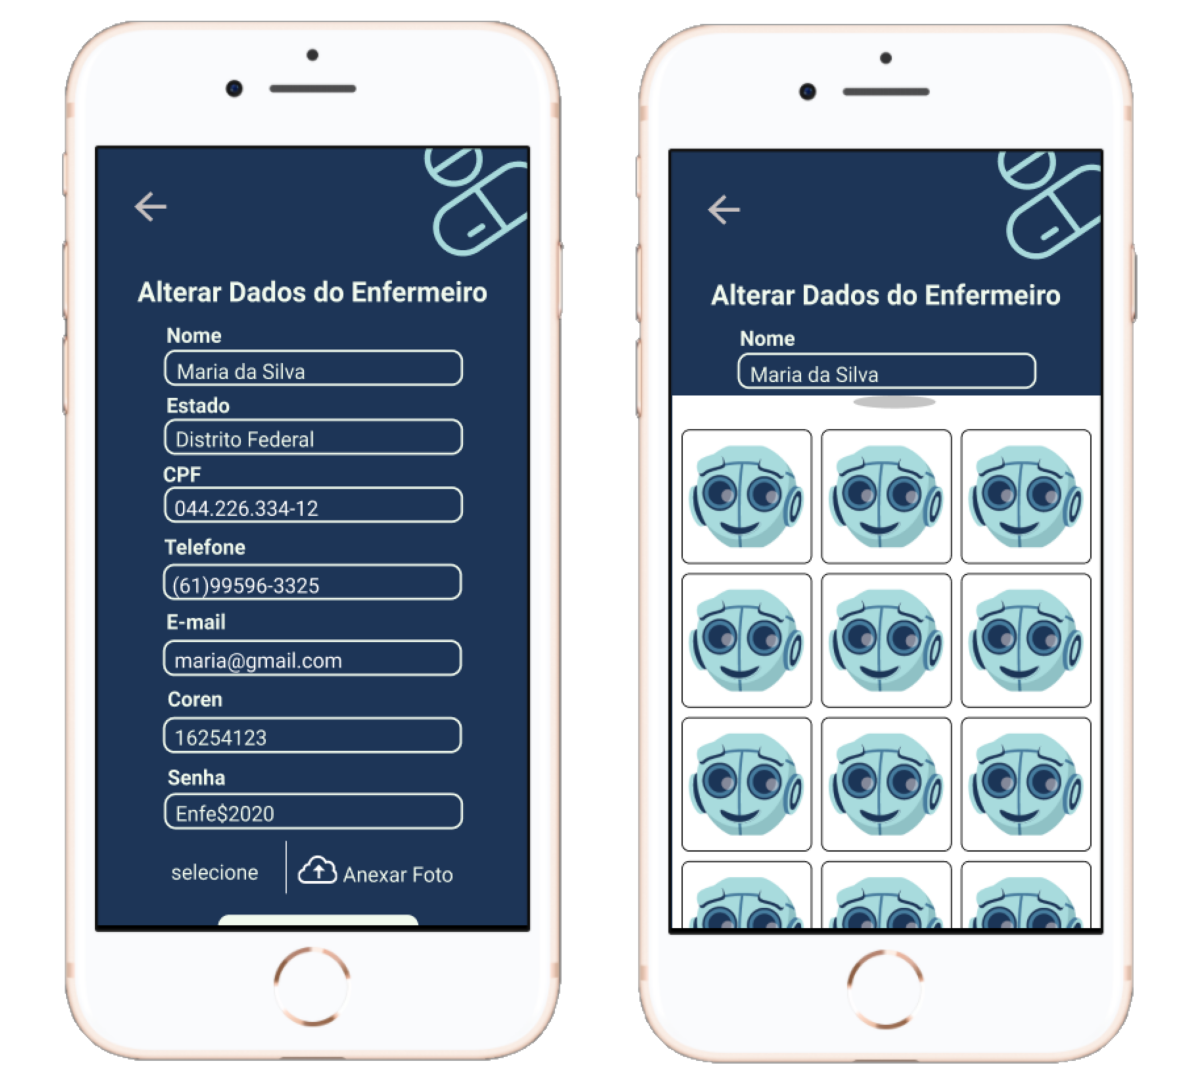
\includegraphics[width=8cm]{figuras/software/Atual_prototipo/Admin_alterarParte1.png}
    \label{fig:prototipo_admin_alterarDados_1}}
    \subfloat[][Tela com foto alterada e \textit{feedback} da alteração]{
    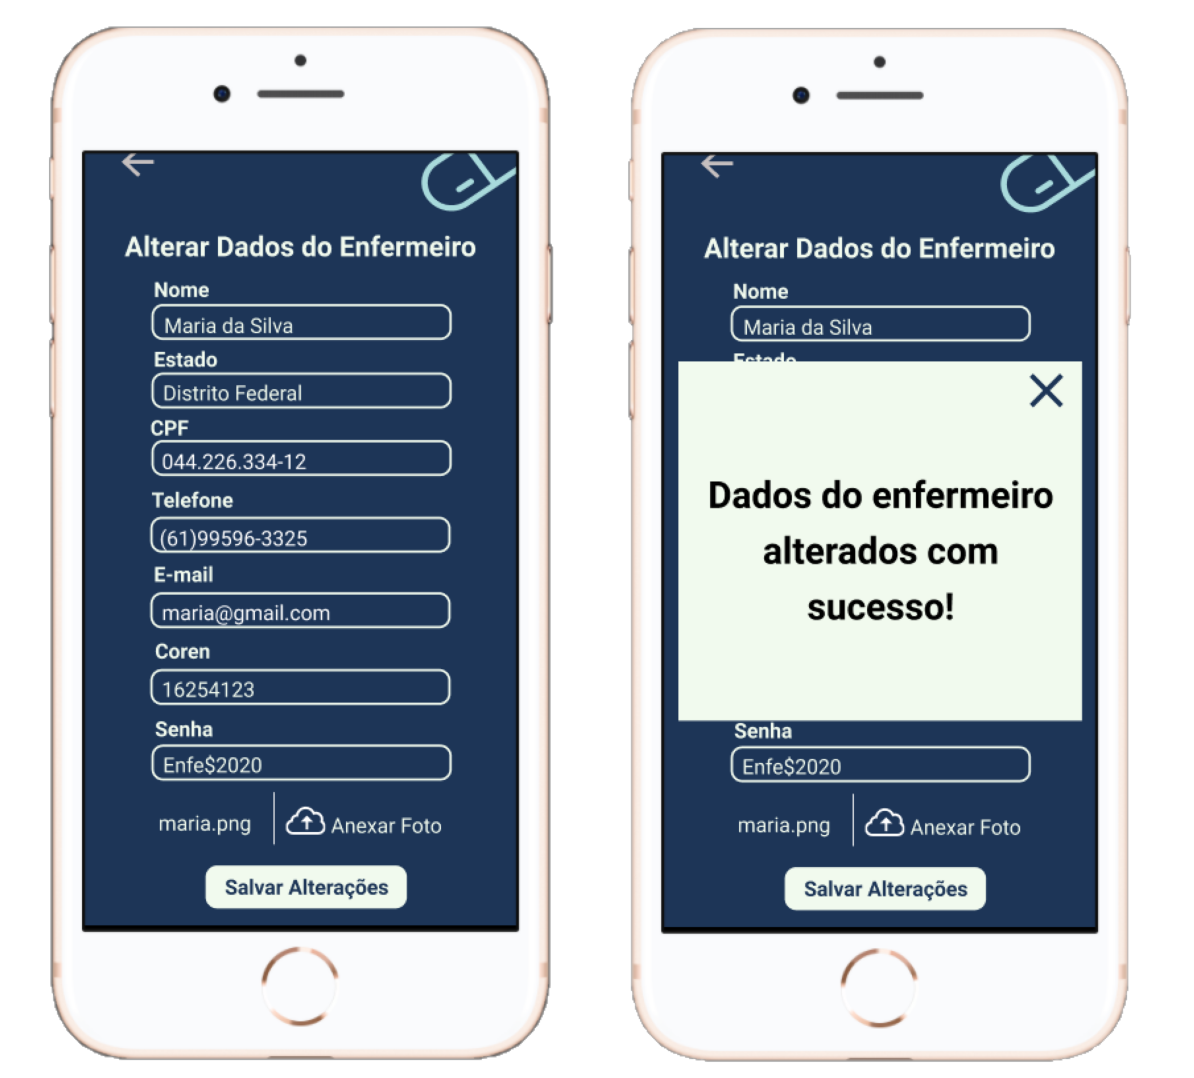
\includegraphics[width=8cm]{figuras/software/Atual_prototipo/Admin_alterarParte2.png}
    \label{fig:prototipo_admin_alterarDados_2}}
    \caption{Administrador - Fluxo para alterar dados}
\end{figure}

\begin{table}[H]
    \centering
    \caption{Tabela de Interações das Telas de Gerenciamento de Cadastro de Enfermeiro}
    \label{tab:interacao-telas-cadast_enfermeiro}
    \begin{adjustbox}{max width = \textwidth}
    % \begin{adjustwidth}{-2,5cm}{}
        \begin{tabular}{|L{4cm}|L{4cm}|L{6cm}|L{4cm}|L{4cm}|}
            \hline
            \rowcolor[HTML]{A8DADC}
            \multicolumn{1}{|c|}{\textbf{Tela}} & \multicolumn{1}{c|}{\textbf{Entrada}} & \multicolumn{1}{c|}{\textbf{Interações}} & \multicolumn{1}{c|}{\textbf{Saída}} & \multicolumn{1}{c|}{\textbf{Alternativo}} \\ \hline
             Tela de Enfermeiros Cadastrados & Botão de Gerenciamento de enfermeiro da tela principal do Administrador & Editar ou Deletar Enfermeiro cadastrado & Ícone de Retornar  & \multicolumn{1}{c|}{---} \\ \hline
             Tela de confirmação de exclusão do enfermeiro & Botão excluir & Clicar em Sim ou Cancelar & Ícone de Retornar & \multicolumn{1}{c|}{---} \\ \hline
             Tela de Confirmação de Exclusão de Cadastro & Botão Sim da tela anterior & \multicolumn{1}{c|}{---} & Botão Voltar & \multicolumn{1}{c|}{---} \\ \hline
             Tela de Editar Cadastro de Enfermeiro & Botão de editar da tela de gerenciamento de cadastro de enfermeiro & Editar todos os dados cadastrais do enfermeiro e alterar foto & Salvar Alterações & \multicolumn{1}{c|}{---} \\ \hline
             \textit{Pop-up} de confirmação de Alteração & Salvar Alterações & \multicolumn{1}{c|}{---} & Icone de Fechar \textit{Pop-up} & \multicolumn{1}{c|}{---} \\ \hline
        \end{tabular}
    % \end{adjustwidth}
    \end{adjustbox}
\end{table}

% \begin{figure}[H]
%     \centering
% \end{center}

% "Funciona" mas nao vale a pena a dor de cabeça pra compilar porque tem muitas poucas imagens; Gif só funciona no adobe acrobat com flash instalado
% Perda de suporte dessa funcionalidade no final de 2020
% \begin{figure}[H]
%     \centering
% \begin{center}
    % \includemedia[width=8cm,activate=pageopen,
    % passcontext,
    % transparent,
    % addresource=figuras/software/animation.mp4,
    % flashvars={source=figuras/software/animation.mp4}
    % ]{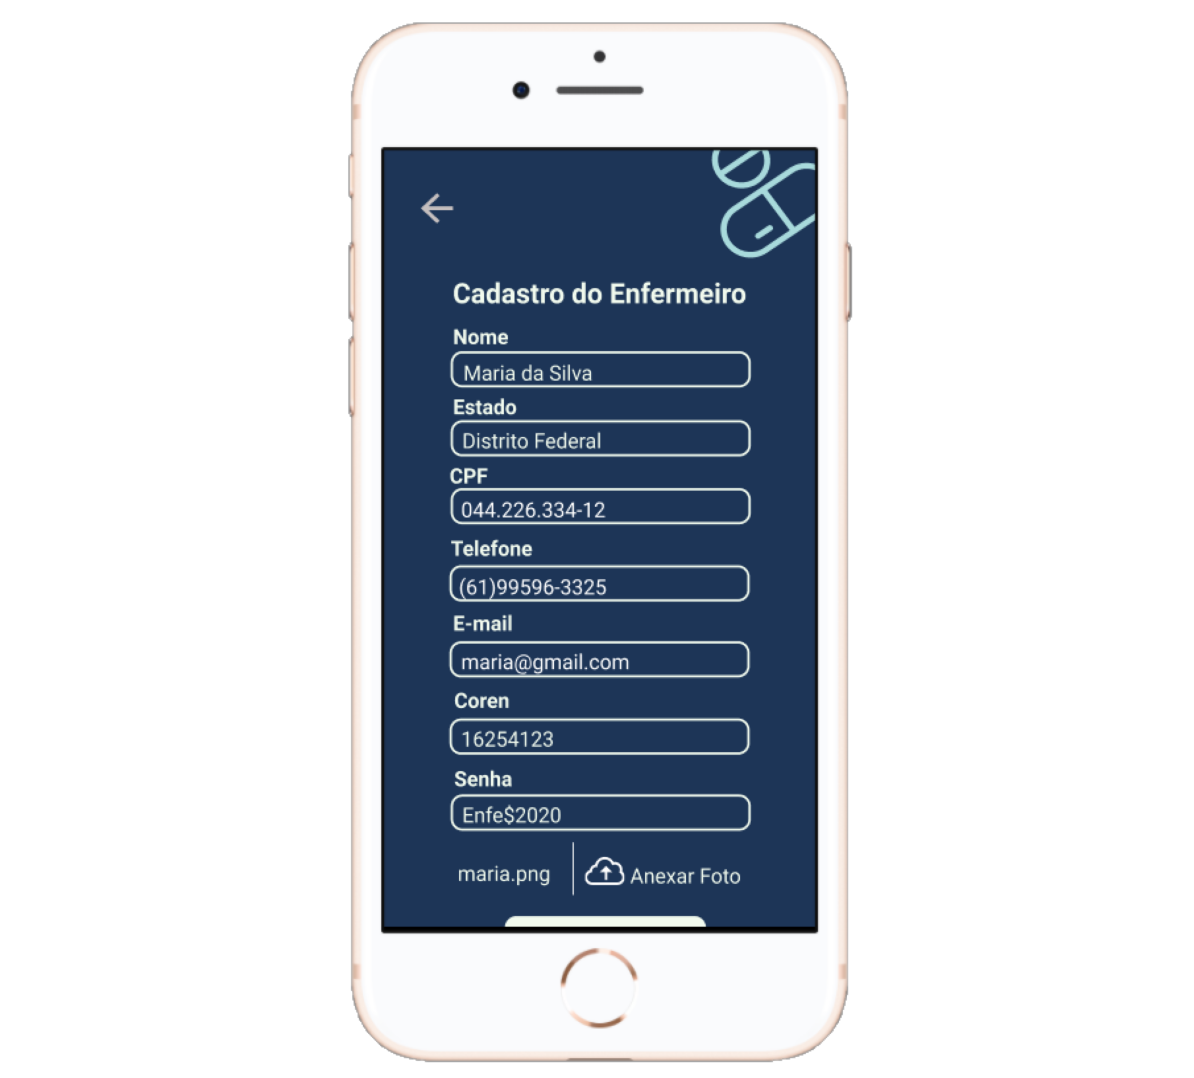
\includegraphics[width=8cm]{figuras/software/Atual_prototipo/Admin_Cadastro1.png}}{VPlayer.swf}
    % \label{fig:prototipo_admin_alterarDadosEnfermeiro}
    % \caption{Administrador - Parte 8}
% \end{center}
    
% \end{figure}

% \subsubsection{Enfermeiro(a)}
\subparagraph*{$\bullet$ Enfermeiro(a)} \hfill
% \subsubsubsection{Menu Inicial e \textit{sidebar}}
\subparagraph*{} $-$ Menu Inicial e \textit{sidebar}

A Fig.\ref{fig:prototipo_enfermeiro_menuInicial_e_Sidebar} apresenta as opções de execução de gerenciamento que o usuário enfermeiro possui permissão dentro da aplicação, bem como o acesso a \textit{sidebar} que possibilita que o usuário possa visualizar os dados pessoais, editar dados cadastrais e sair da aplicação.

\begin{figure}[H]
    \centering
    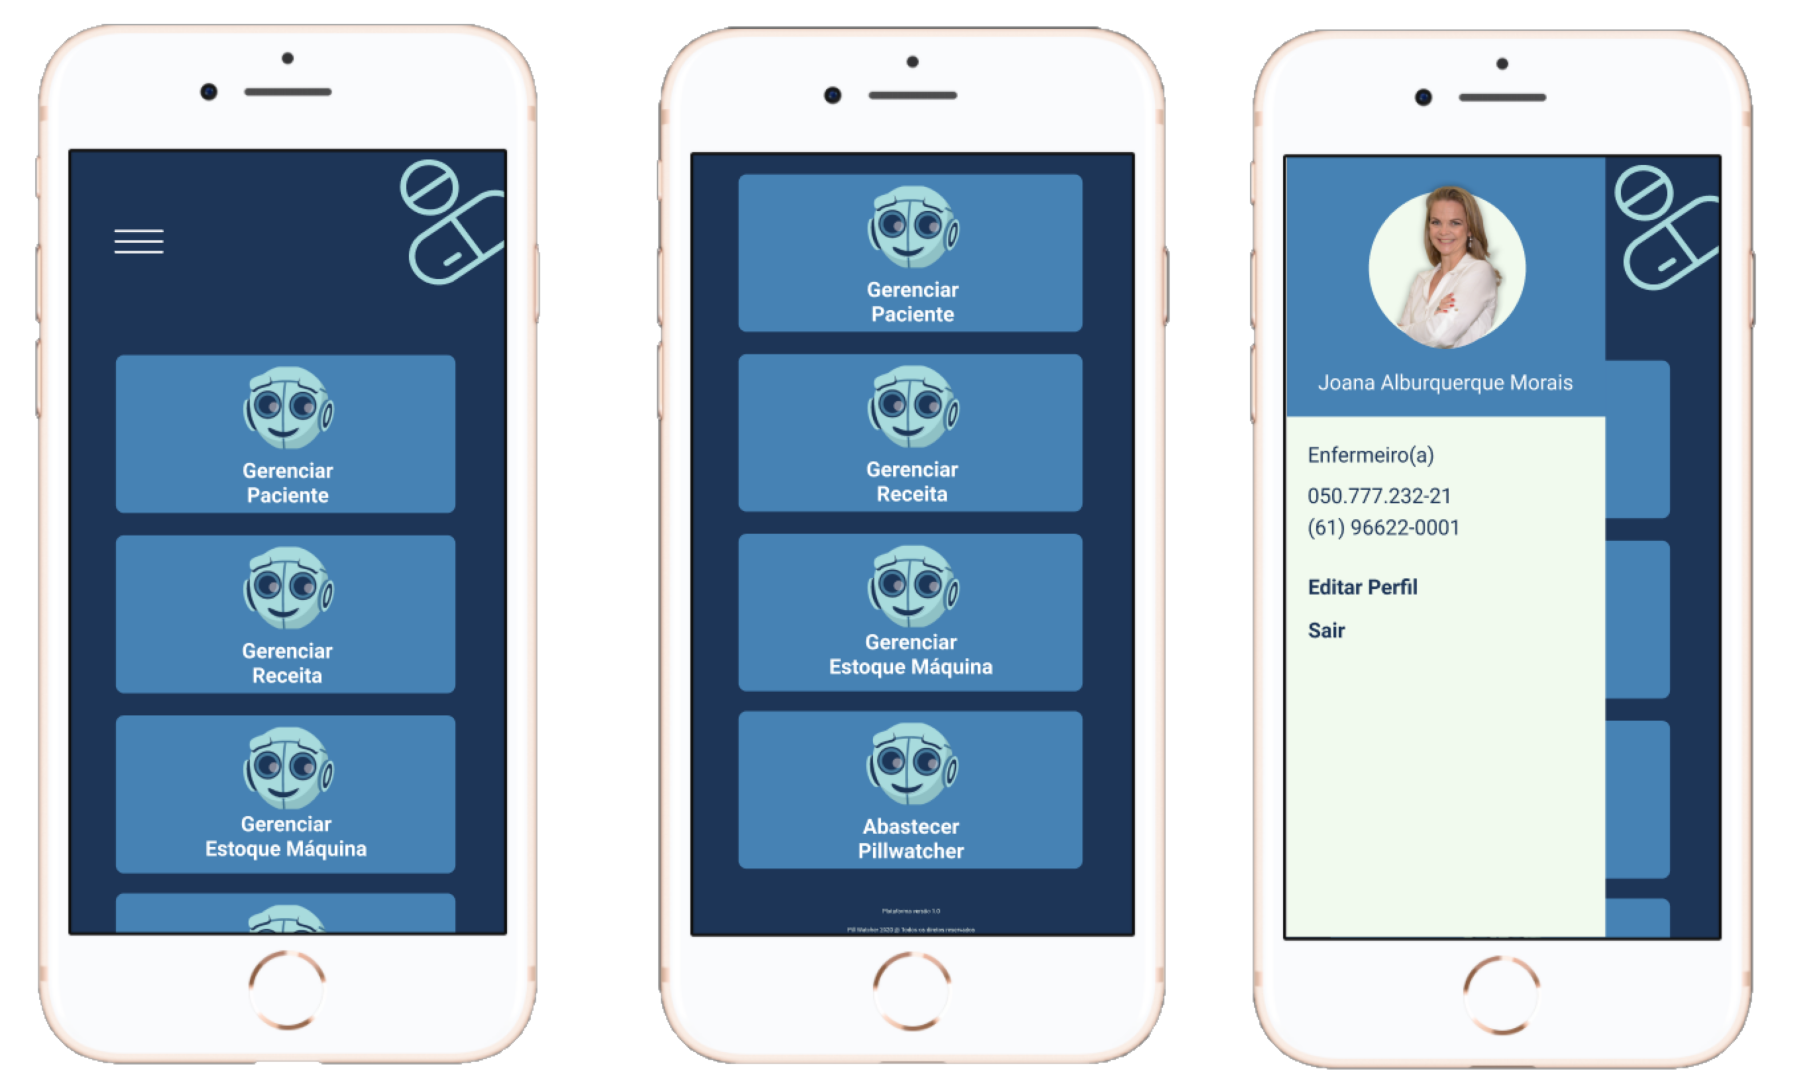
\includegraphics[width=15cm]{figuras/software/Atual_prototipo/Enfermeiro_TelaInicial_e_Sidebar.png}
    \caption{Enfermeiro - Menu inicial e \textit{sidebar}}
    \label{fig:prototipo_enfermeiro_menuInicial_e_Sidebar}
\end{figure}

Na sequencia, a Fig. \ref{fig:prototipo_enfermeiro_alterarDados} representa a tela de edição de perfil que permitirá ao usuário enfermeiro, por meio do acesso a opção de `editar dados' da \emph{sidebar} possa alterar seus dados pessoais cadastrados na aplicação, bem como adicionar uma nova foto de perfil e receber um \textit{feedback} com relação ao sucesso na execução da alteração de dados na aplicação

\begin{figure}[H]
    \centering
    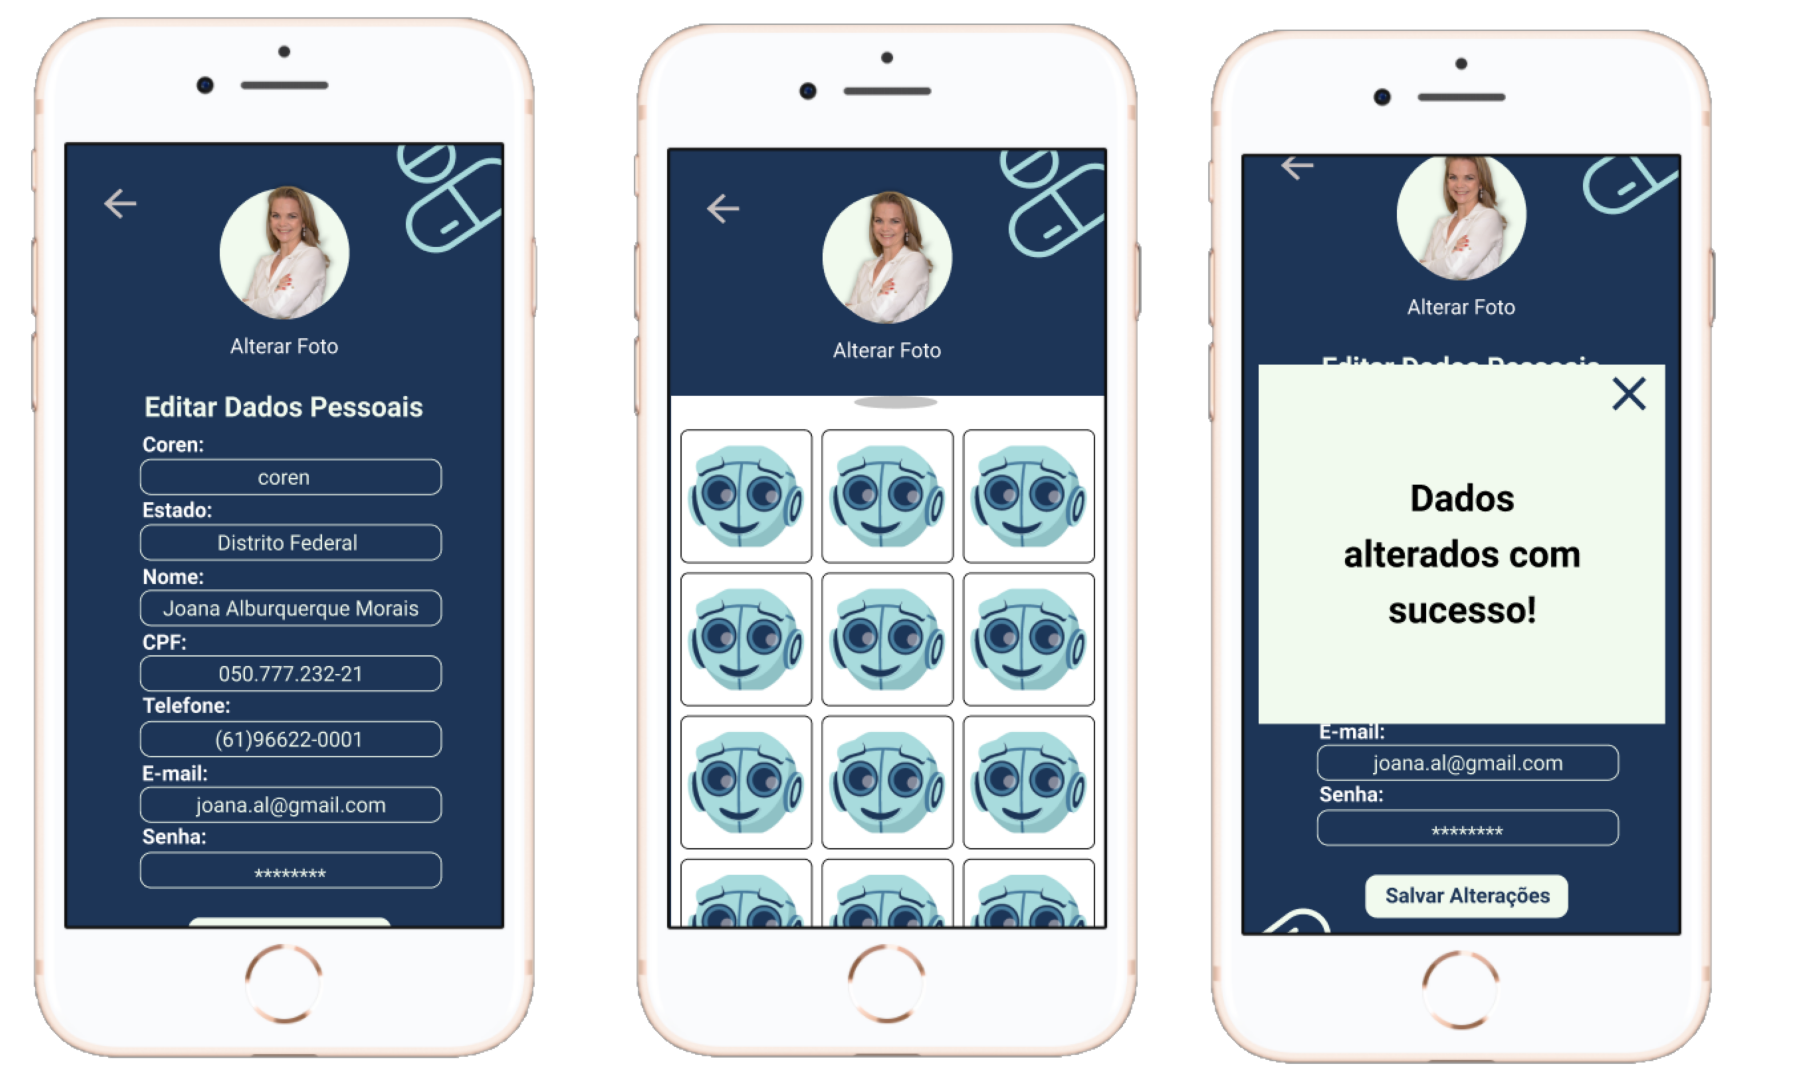
\includegraphics[width=15cm]{figuras/software/Atual_prototipo/Enfermeiro_alterarDados.png}
    \caption{Enfermeiro - Fluxo de alterar dados}
    \label{fig:prototipo_enfermeiro_alterarDados}
\end{figure}

\begin{table}[H]
    \centering
    \caption{Tabela de Interações das Telas Principais de Administrador}
    \label{tab:interacao-telas-adm_principais}
    \begin{adjustbox}{max width = \textwidth}
    % \begin{adjustwidth}{-2,5cm}{}
        \begin{tabular}{|L{5cm}|L{4cm}|L{6cm}|L{4cm}|L{4cm}|}
            \hline
            \rowcolor[HTML]{A8DADC}
            \multicolumn{1}{|c|}{\textbf{Tela}} & \multicolumn{1}{c|}{\textbf{Entrada}} & \multicolumn{1}{c|}{\textbf{Interações}} & \multicolumn{1}{c|}{\textbf{Saída}} & \multicolumn{1}{c|}{\textbf{Alternativo}} \\ \hline
             Tela Principal - Enfermeiro & Realizando Login na aplicação & Clicar no botão de acesso a \textit{sidebar}, clicar nos botões de acesso as ações principais do enfermeiro & \multicolumn{1}{c|}{---}  & \multicolumn{1}{c|}{---} \\ \hline
             \textit{Sidebar} - Enfermeiro & Acessando Menu superior esquerdo da Tela Principal do enfermeiro & Clicar na opção de edição de dados pessoais, clicar na opção de sair  & \multicolumn{1}{c|}{---} & \multicolumn{1}{c|}{---} \\ \hline
             Tela de Editar Dados Pessoais & Usuário clicar no botão de editar dados & Alterar dados de cadastro & \multicolumn{1}{c|}{Botão Salvar} & \multicolumn{1}{c|}{---} \\ \hline
        \end{tabular}
    % \end{adjustwidth}
    \end{adjustbox}
\end{table}

% \subsubsubsection{Gerenciar paciente}
\subparagraph*{} $-$ Gerenciar paciente

A Fig. \ref{fig:prototipo_enfermeiro_menuInicialGerenciarPacientes} representa as telas iniciais do fluxo de gerenciamento dos pacientes, as quais, possibilitaram o usuário enfermeiro editar e/ou excluir um cadastro de paciente existente na aplicação e receber um \textit{feedback} sobre as ações executadas e a Fig. \ref{fig:prototipo_enfermeiro_deletarPaciente} representa o fluxo para deletar um enfermeiro cadastrado.

\begin{figure}[H]
    \centering
    \subfloat[][Menu inicial de gerenciar pacientes e busca por um paciente]{
    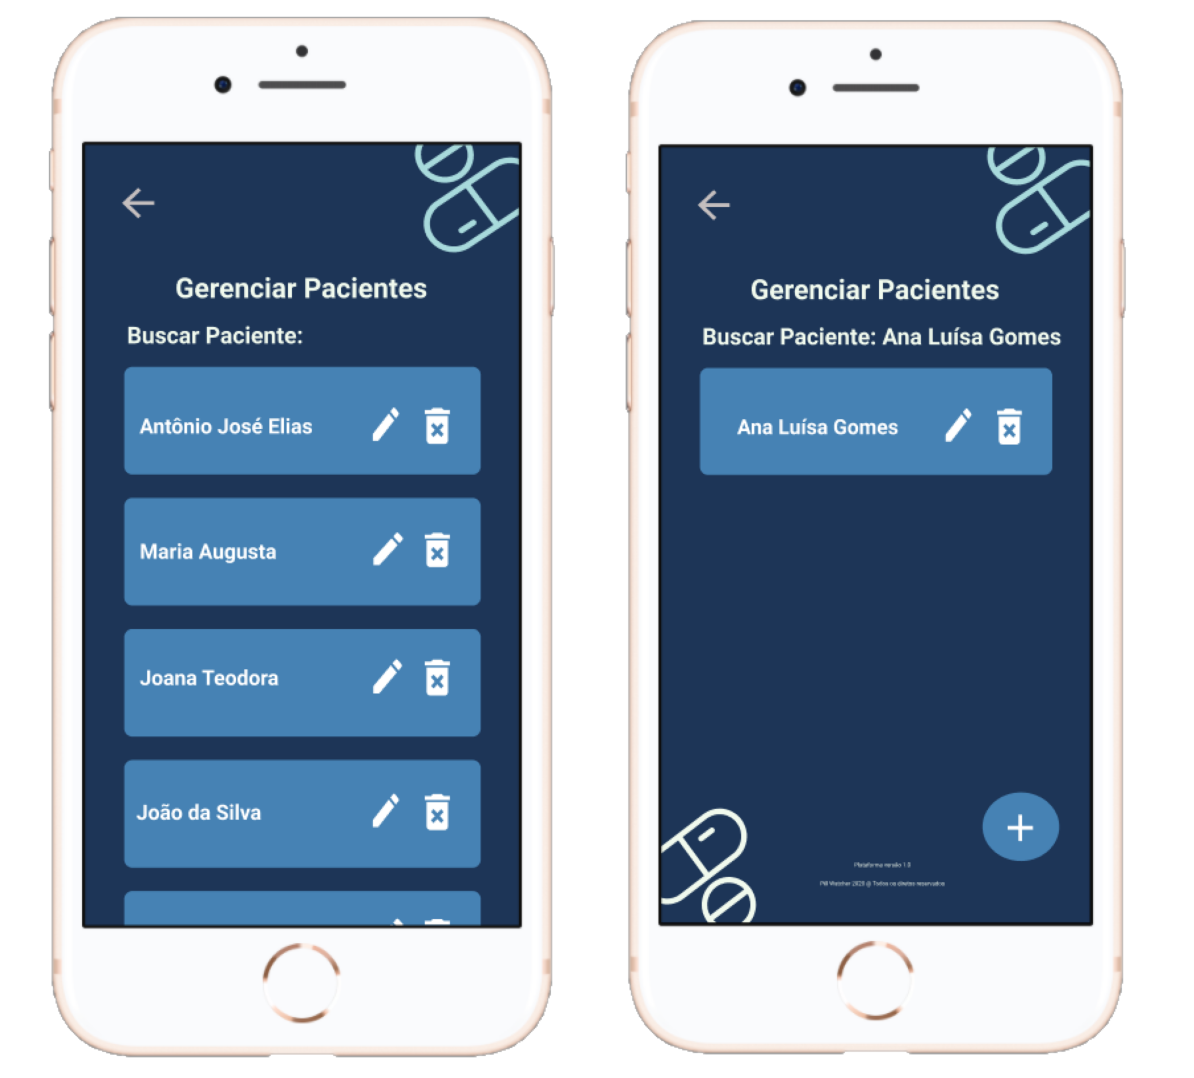
\includegraphics[width=8cm]{figuras/software/Atual_prototipo/Enfermeiro_gerenciarPacientes_1.png}
     \label{fig:prototipo_enfermeiro_menuInicialGerenciarPacientes}}
    \subfloat[][fluxo para deletar um paciente do \textit{app}]{
    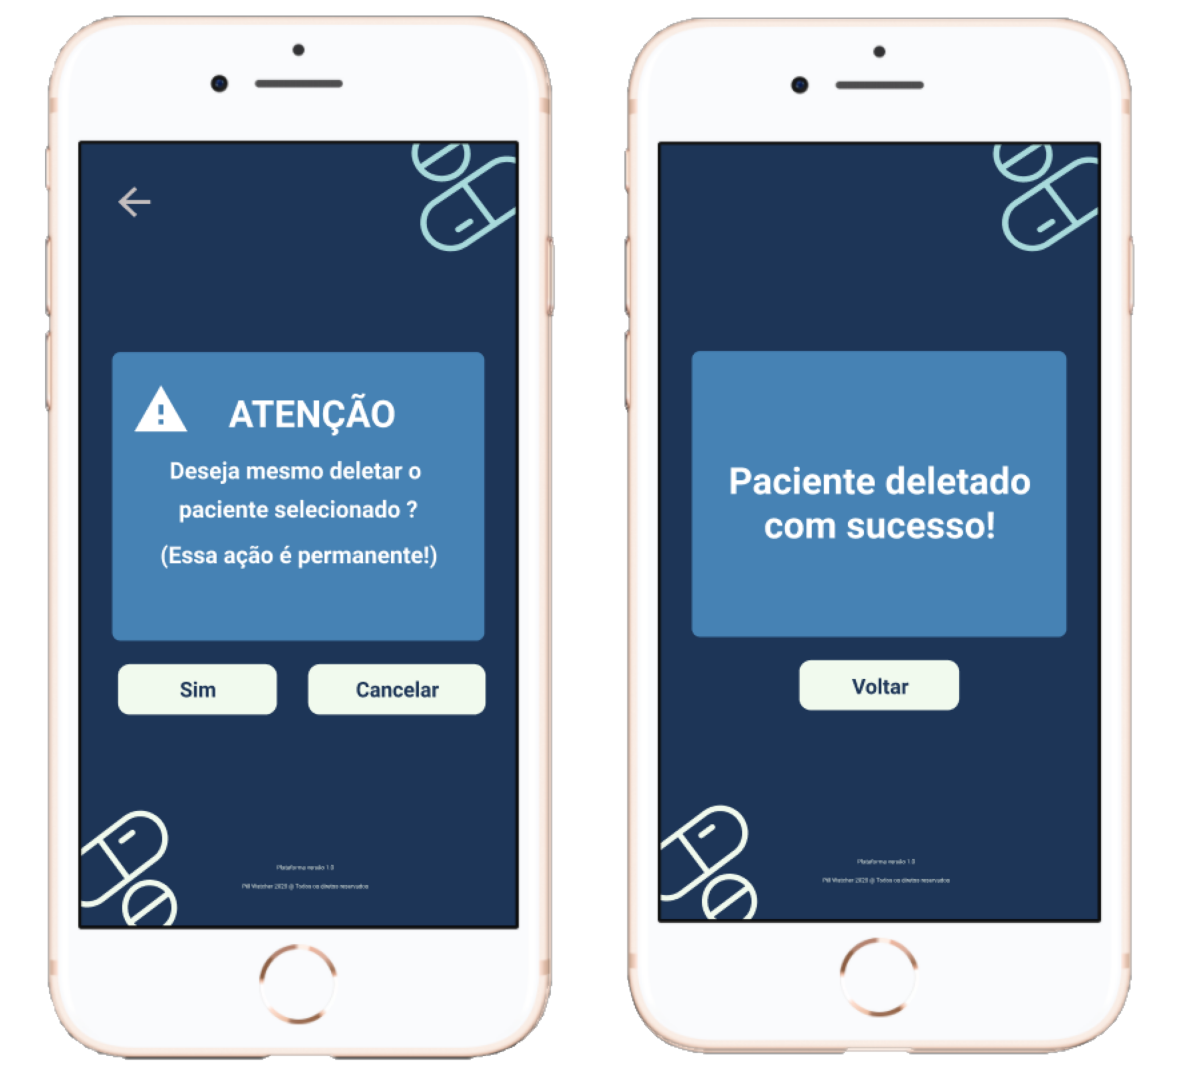
\includegraphics[width=8cm]{figuras/software/Atual_prototipo/Enfermeiro_gerenciarPacientes_2.png}
    \label{fig:prototipo_enfermeiro_deletarPaciente}}
    \caption{Enfermeiro - Tela inicial, busca e fluxo de deletar paciente}
\end{figure}

A Fig. \ref{fig:prototipo_enfermeiro_alterarDadosPaciente_1} apresenta a primeira parte do fluxo para editar dados do paciente cadastrado.

\begin{figure}[H]
    \centering
    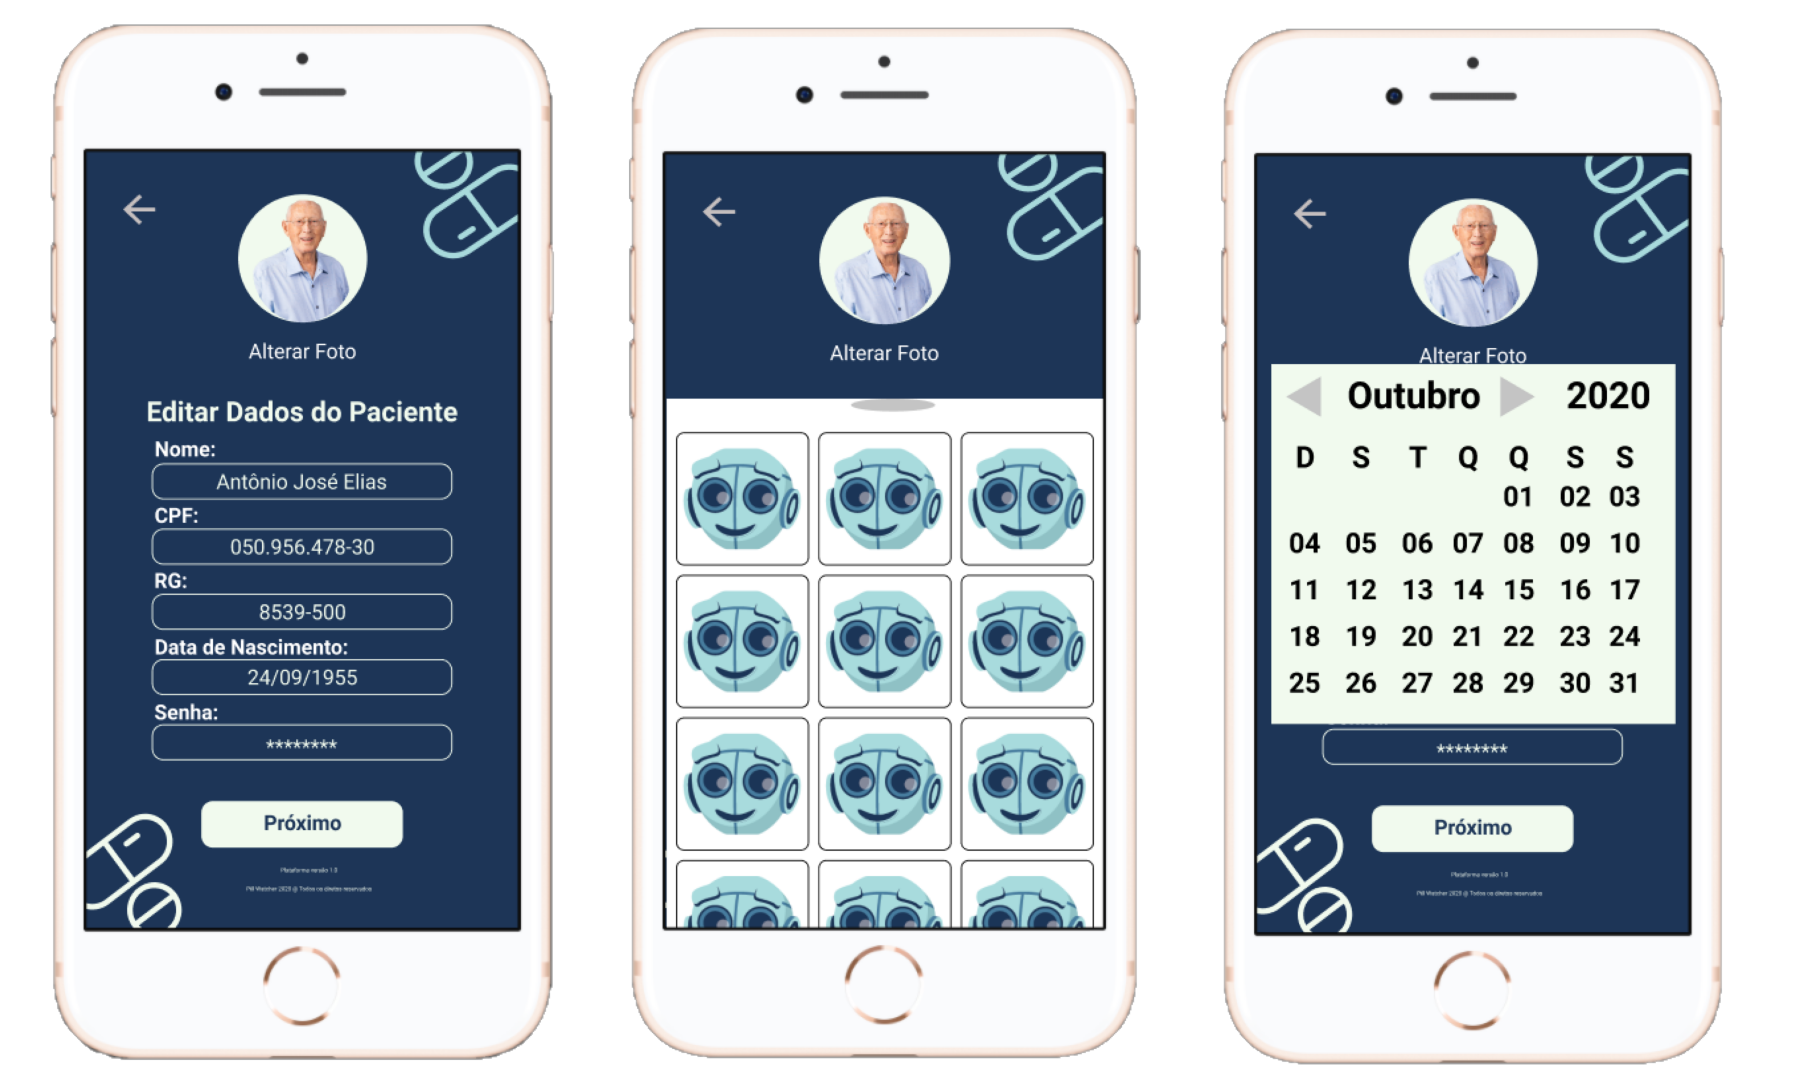
\includegraphics[width=15cm]{figuras/software/Atual_prototipo/Enfermeiro_editarDadosPaciente_1.png}
    \caption{Enfermeiro - Parte 1 do fluxo de alterar dados de um paciente}
     \label{fig:prototipo_enfermeiro_alterarDadosPaciente_1}
    
\end{figure}

A segunda parte do fluxo de edição do cadastro de um paciente, conforme apresentado na Fig. \ref{fig:prototipo_enfermeiro_alterarDadosPaciente_2}, baseia-se na edição das informações cadastrais do familiar vinculado ao paciente, bem como o recebimento da confirmação de conclusão de alterações realizadas.

\begin{figure}[H]
    \centering
    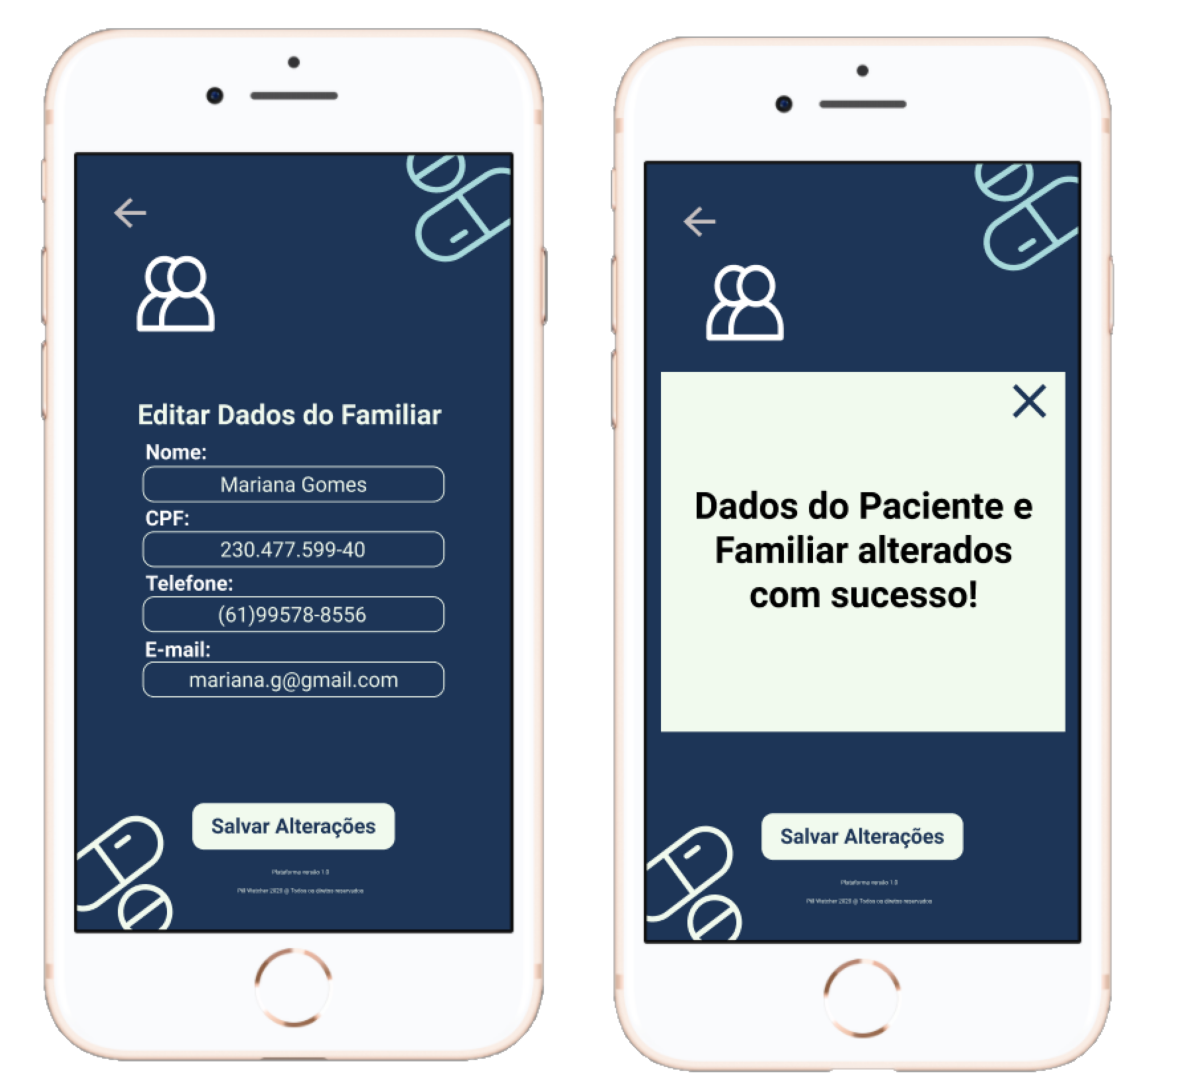
\includegraphics[width=12cm]{figuras/software/Atual_prototipo/Enfermeiro_editarDadosPaciente_2.png}
    \caption{Enfermeiro - Parte 2 do fluxo de alterar dados de um paciente}
    \label{fig:prototipo_enfermeiro_alterarDadosPaciente_2}
\end{figure}

As Fig. \ref{fig:prototipo_enfermeiro_cadastroPaciente_1} e \ref{fig:prototipo_enfermeiro_cadastroPaciente_2} exibem o fluxo a ser seguido para um enfermeiro cadastrar um paciente no aplicativo.

\begin{figure}[H]
    \centering
    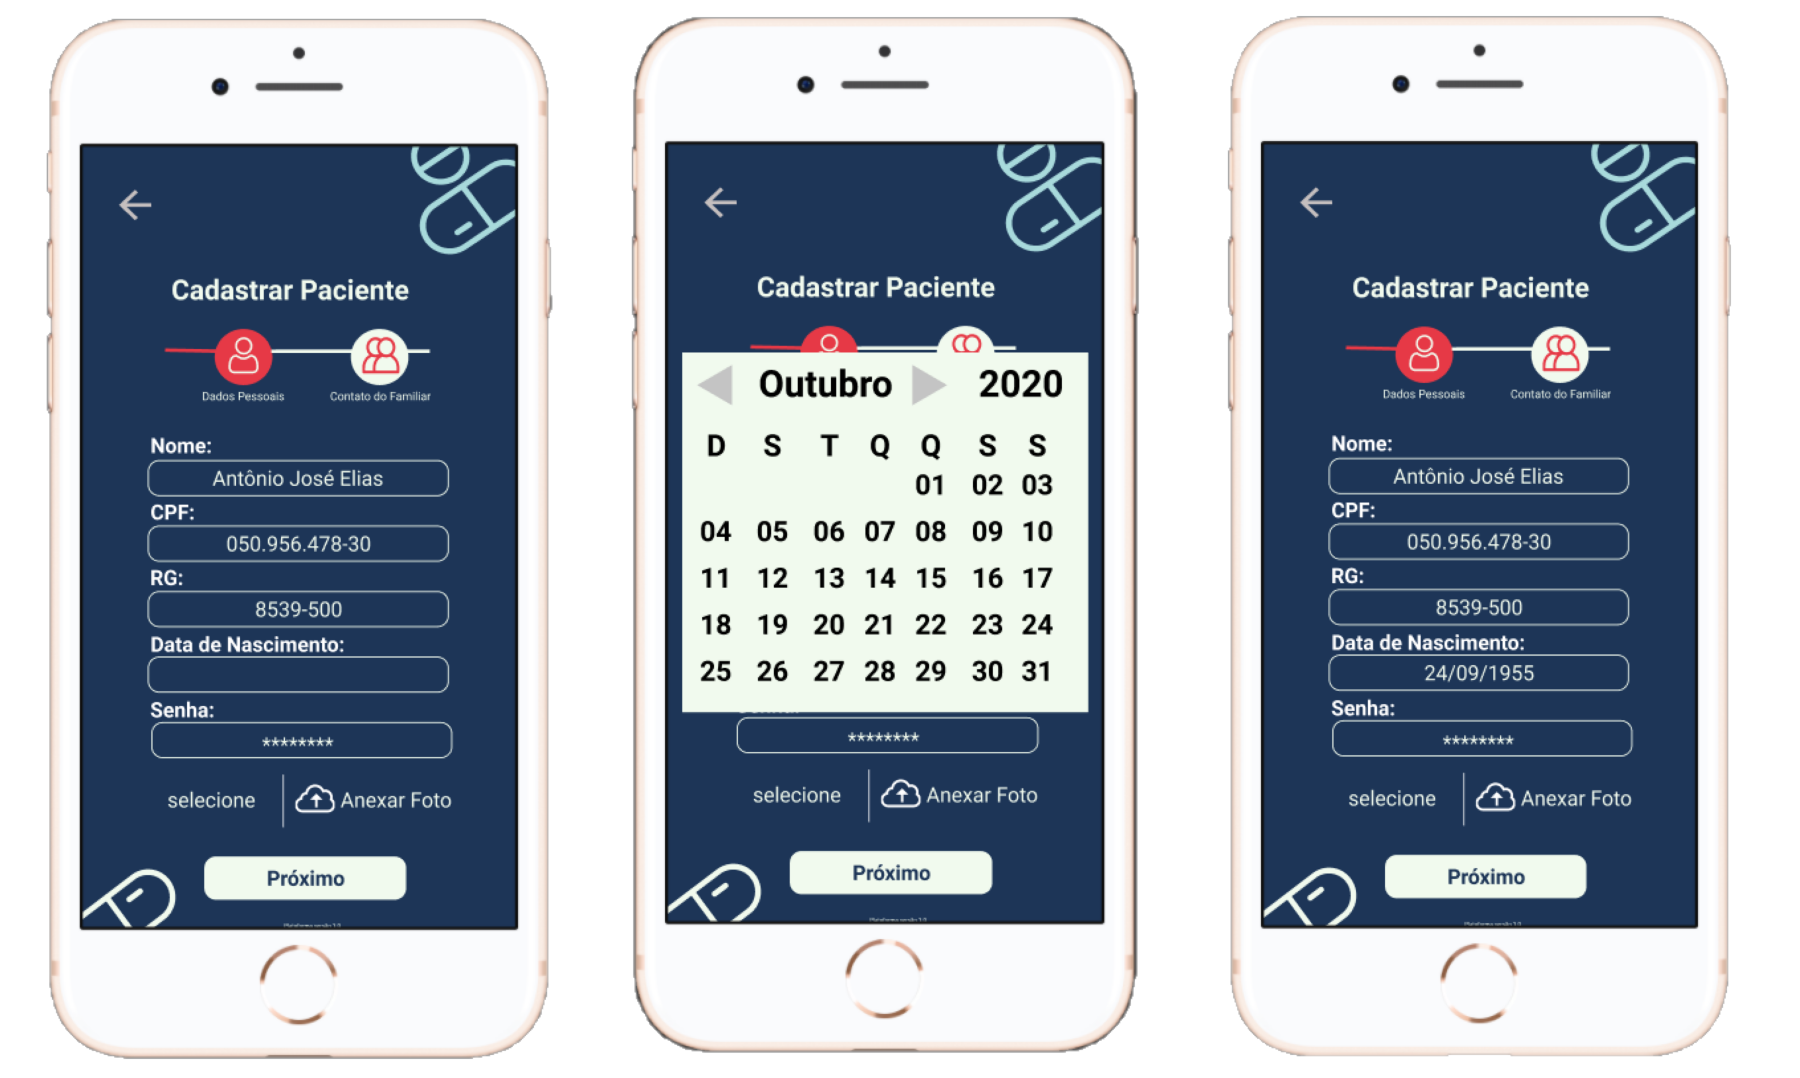
\includegraphics[width=15cm]{figuras/software/Atual_prototipo/Enfermeiro_cadastroPaciente_1.png}
    \caption{Enfermeiro - Parte 1 do fluxo para cadastrar um paciente}
    \label{fig:prototipo_enfermeiro_cadastroPaciente_1}
\end{figure}

\begin{figure}[H]
    \centering
    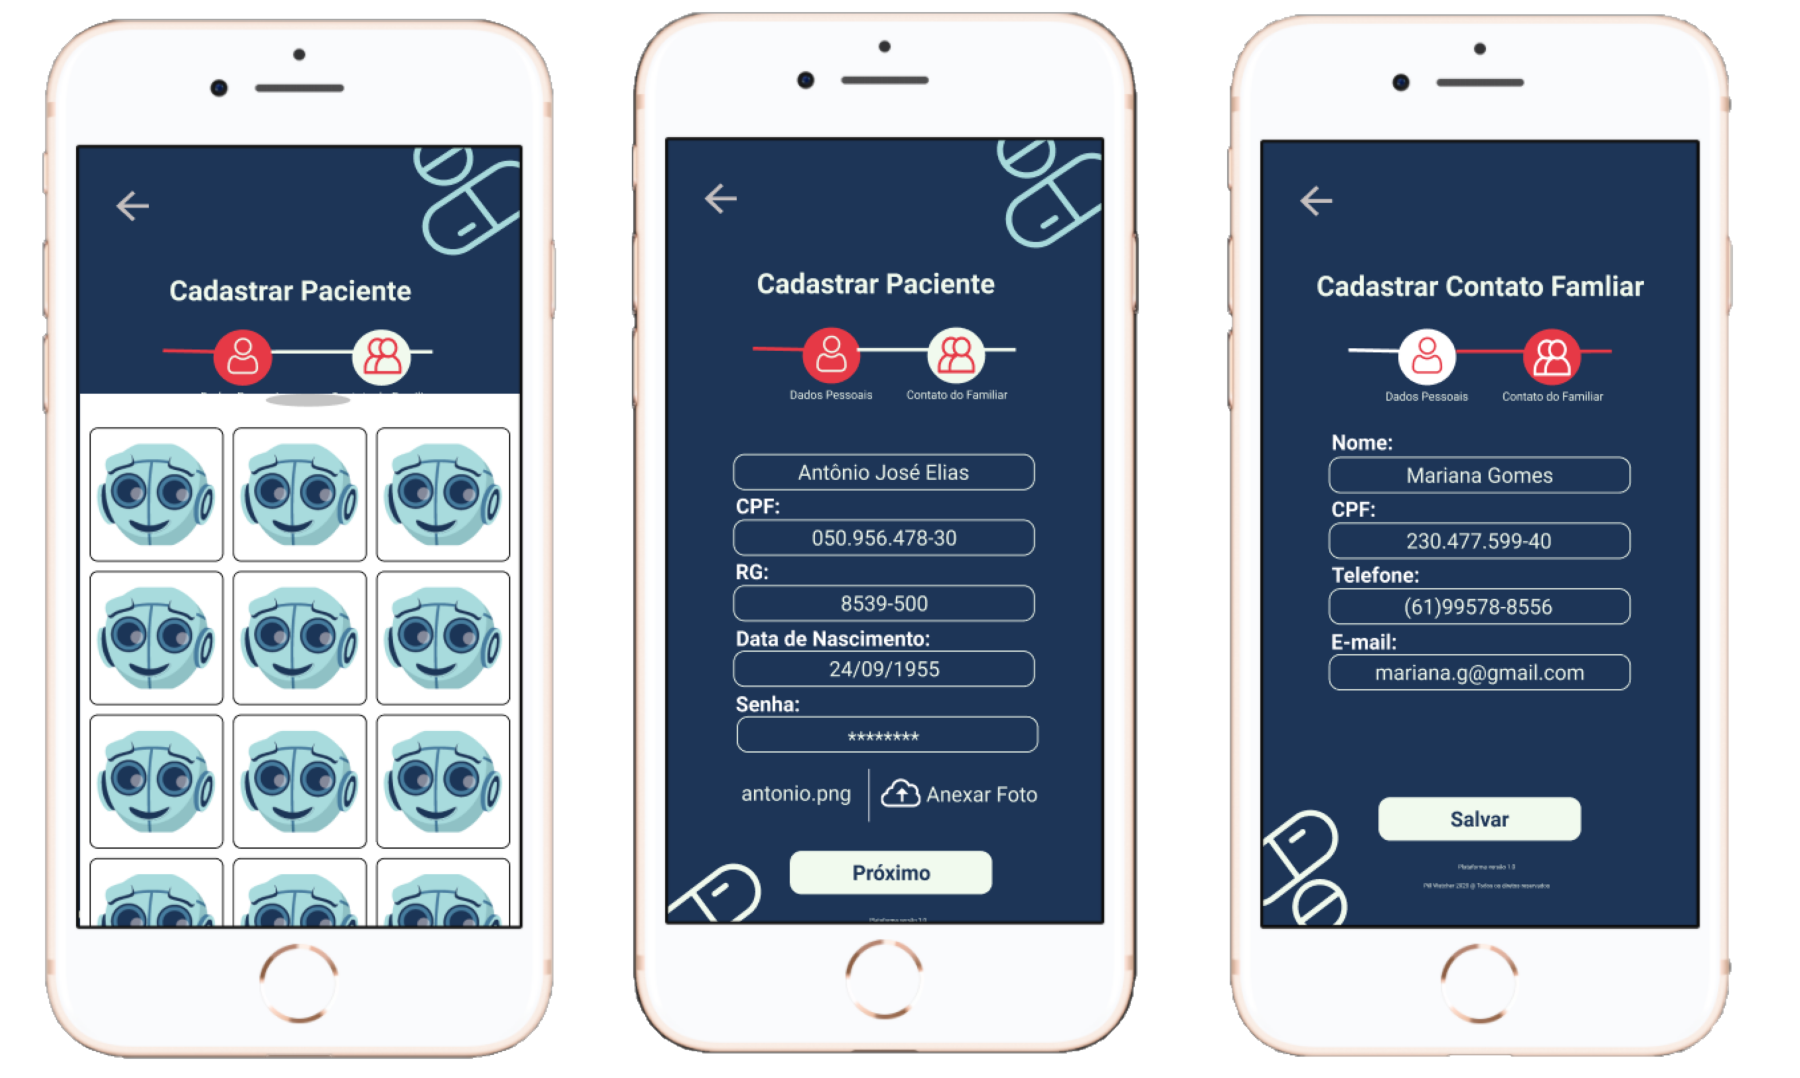
\includegraphics[width=15cm]{figuras/software/Atual_prototipo/Enfermeiro_cadastroPaciente_2.png}
    \caption{Enfermeiro - Parte 2 do fluxo para cadastrar um paciente}
    \label{fig:prototipo_enfermeiro_cadastroPaciente_2}
\end{figure}


\begin{table}[H]
    \centering
    \caption{Tabela de Interações das Telas de Gerenciamento de Cadastro de Paciente}
    \label{tab:interacao-telas-gerenciar-paciente}
    \begin{adjustbox}{max width = \textwidth}
    % \begin{adjustwidth}{-2,5cm}{}
        \begin{tabular}{|L{5cm}|L{6cm}|L{4cm}|L{4cm}|L{4cm}|}
            \hline
            \rowcolor[HTML]{A8DADC}
            \multicolumn{1}{|c|}{\textbf{Tela}} & \multicolumn{1}{c|}{\textbf{Entrada}} & \multicolumn{1}{c|}{\textbf{Interações}} & \multicolumn{1}{c|}{\textbf{Saída}} & \multicolumn{1}{c|}{\textbf{Alternativo}} \\ \hline
             Tela de Pacientes Cadastrados  & Botão de Gerenciamento de Paciente da tela principal do Enfermeiro & Buscar por paciente, editar ou deletar o paciente cadastrado & Ícone de Retornar  & \multicolumn{1}{c|}{---} \\ \hline
             Tela de confirmação de exclusão do paciente & Botão excluir & Clicar em Sim ou Cancelar & Ícone de Retornar & \multicolumn{1}{c|}{---} \\ \hline
             Tela de Confirmação de Exclusão de Cadastro de Paciente & Botão Sim da tela anterior & \multicolumn{1}{c|}{---} & Botão Voltar & \multicolumn{1}{c|}{---} \\ \hline
             Tela de Editar Cadastro de Paciente & Botão de editar da tela de gerenciamento de cadastro de Paciente & Editar todos os dados cadastrais do Paciente e alterar foto & Botão `Próximo' & \multicolumn{1}{c|}{---} \\ \hline
             Tela de Editar Cadastro de Familiar & Botão `Próximo' da tela anterior & Editar todos os dados cadastrais do Familiar e alterar foto & Botão `Salvar' & \multicolumn{1}{c|}{---} \\ \hline
        \end{tabular}
    % \end{adjustwidth}
    \end{adjustbox}
\end{table}

% \subsubsubsection{Gerenciar receita}
\subparagraph*{} $-$ Gerenciar receita

A Fig. \ref{fig:prototipo_enfermeiro_gerenciarReceita_1} representa a tela composta pela lista de receitas cadastradas na aplicação, bem como as opções de visualizar, editar e deletar uma receita individua. A Fig. \ref{fig:prototipo_enfermeiro_gerenciarReceita_2} expõe o modo de visualização de uma receita individual e suas respectivas informações cadastradas.

\begin{figure}[H]
    \centering
    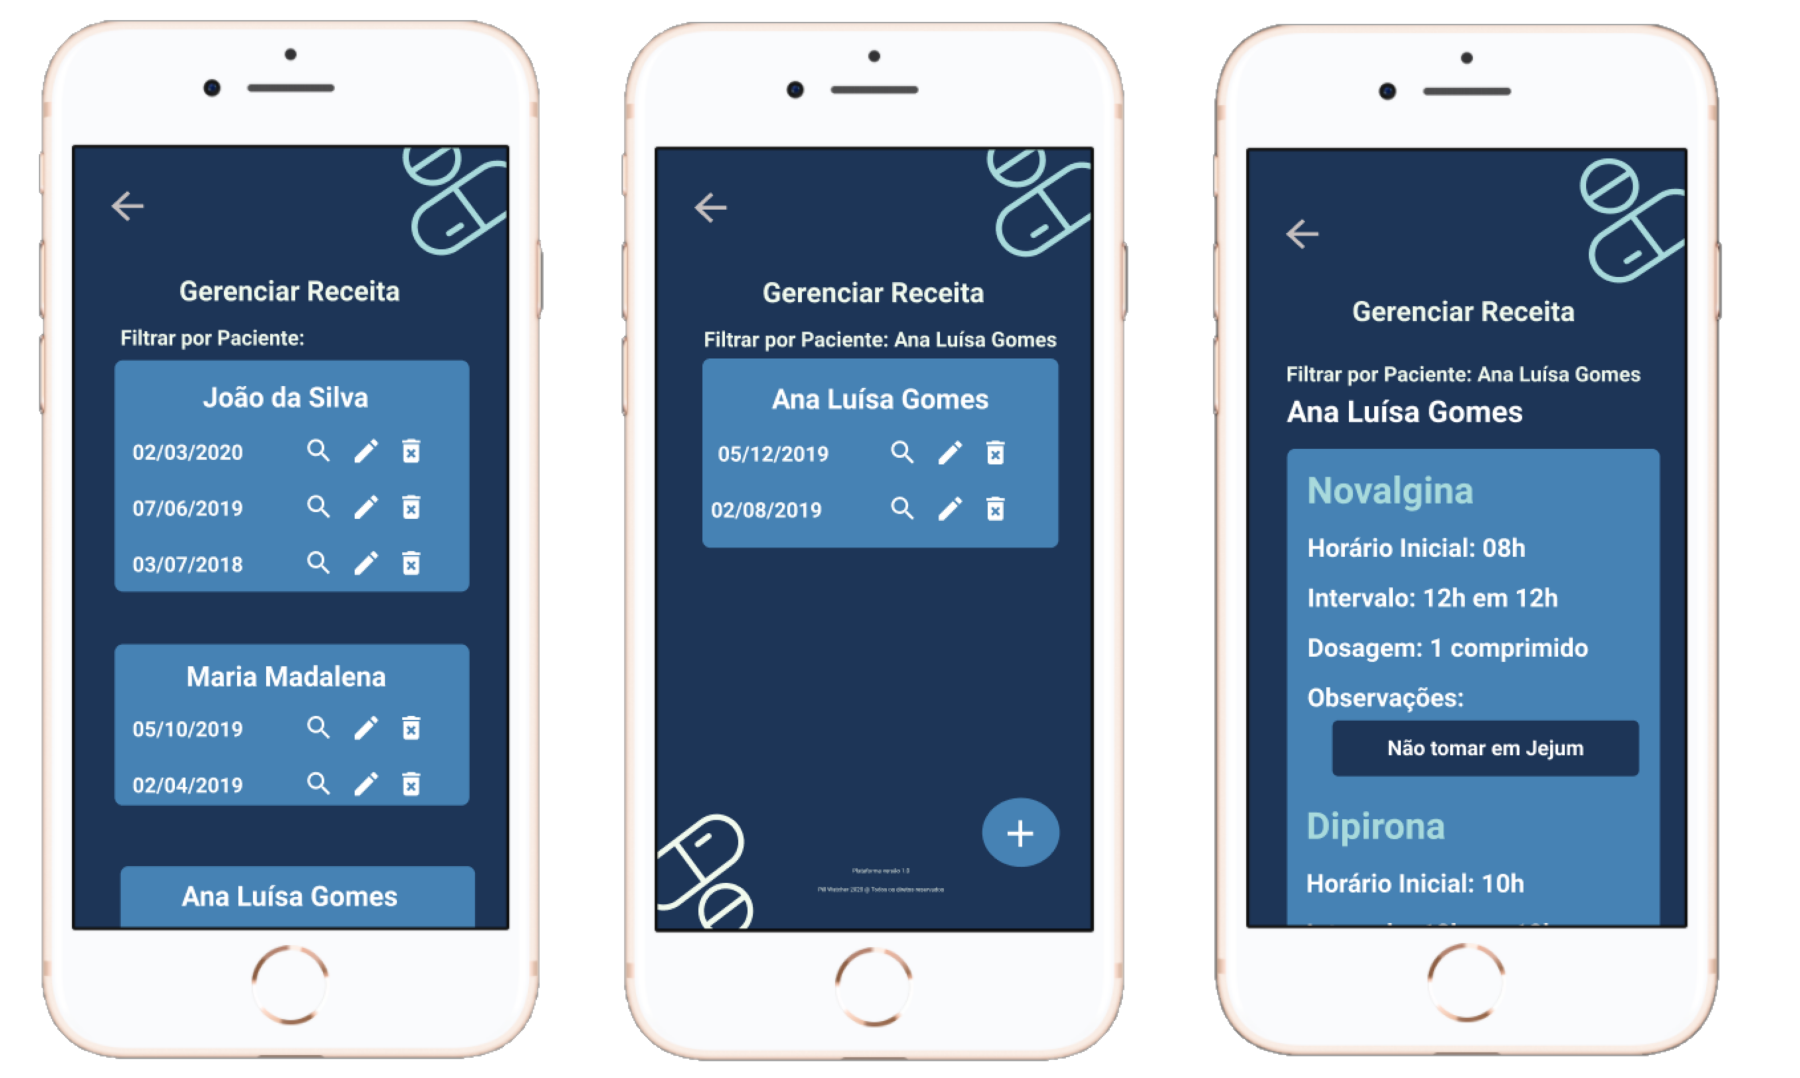
\includegraphics[width=15cm]{figuras/software/Atual_prototipo/Enfermeiro_gerenciarReceita_1.png}
    \caption{Enfermeiro - Tela inicial de gerenciar receita, busca filtrada pelo paciente e visualização da receita}
    \label{fig:prototipo_enfermeiro_gerenciarReceita_1}
\end{figure}

\begin{figure}[H]
    \centering
    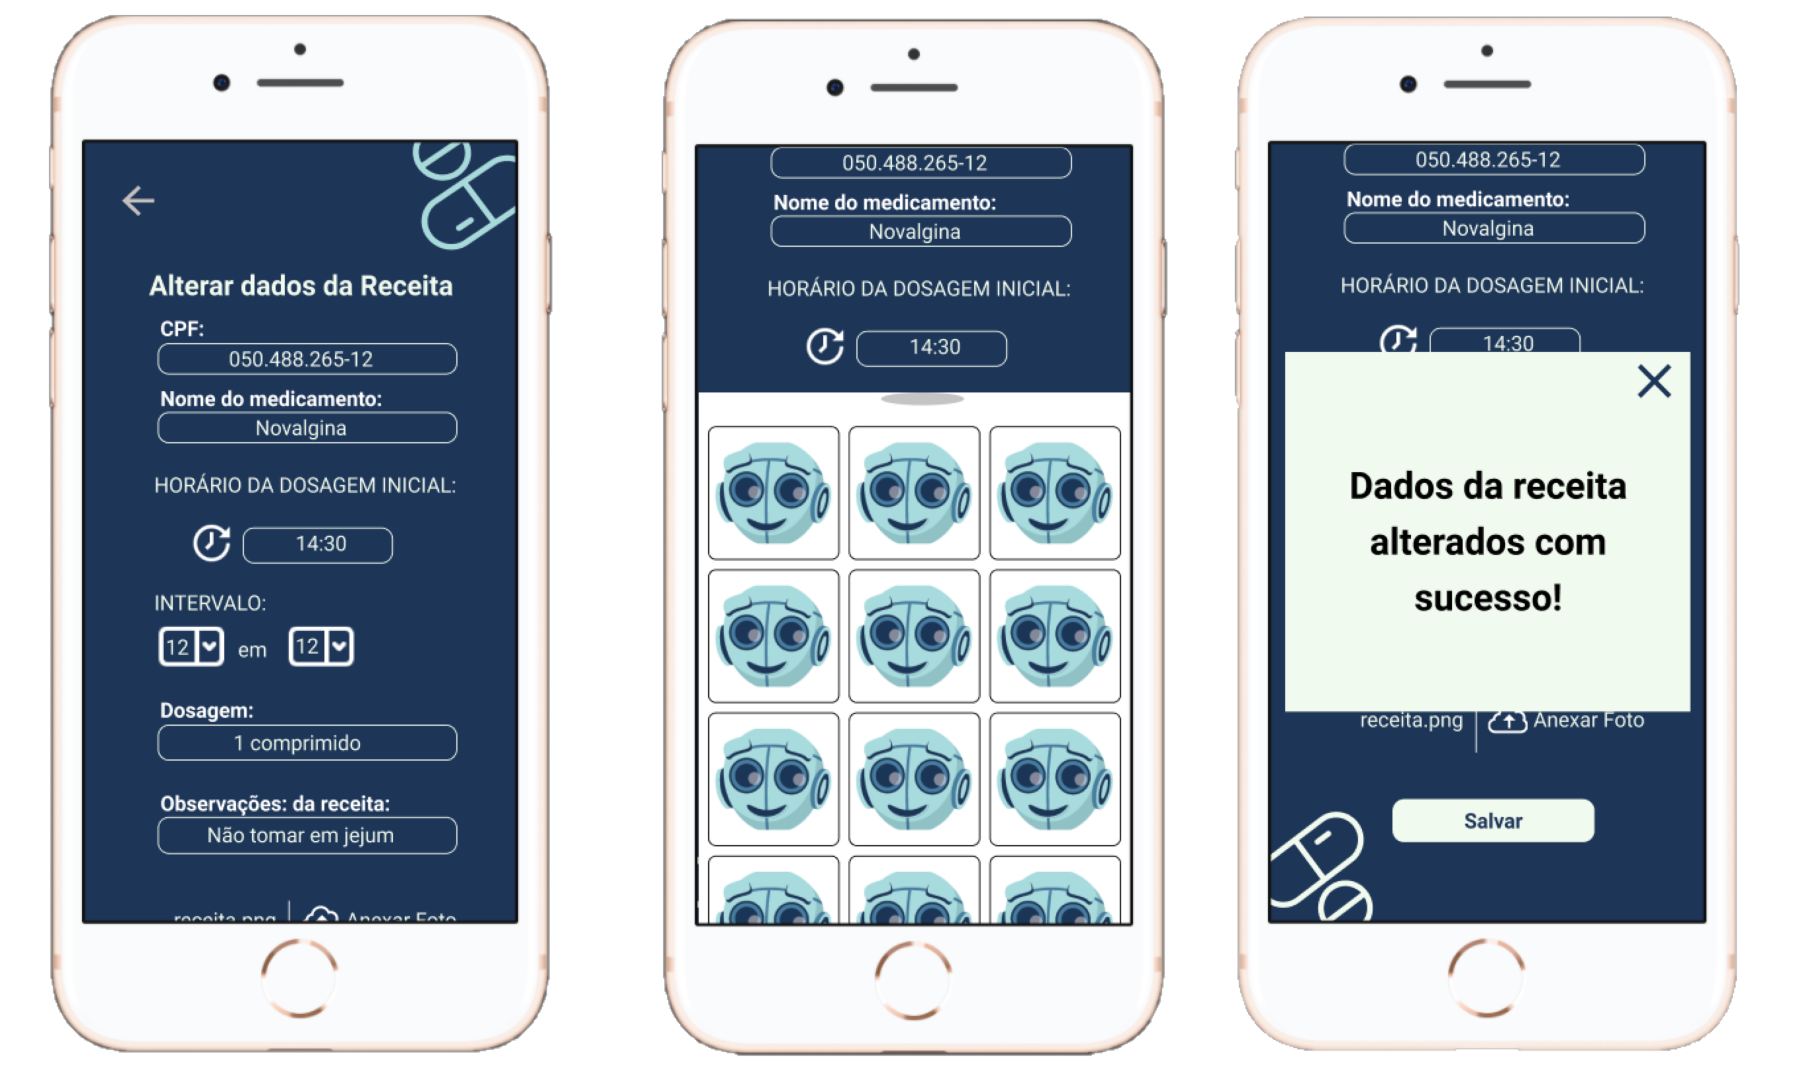
\includegraphics[width=15cm]{figuras/software/Atual_prototipo/Enfermeiro_gerenciarReceita_2.png}
    \caption{Enfermeiro - Fluxo de alteração de dados de uma receita}
    \label{fig:prototipo_enfermeiro_gerenciarReceita_2}
\end{figure}

Na Fig. \ref{fig:prototipo_enfermeiro_gerenciarReceita_3} é apresentado a tela de edição dos dados da receita cadastrados anteriormente, bem como a forma a ser anexado um registro do documento original. Na Fig. \ref{fig:prototipo_enfermeiro_gerenciarReceita_4} é exibido um \textit{pop-up} de confirmação das alterações realizadas no cadastro da receita do paciente.

\begin{figure}[H]
    \centering
    \subfloat[][Fluxo para deletar uma receita]{
    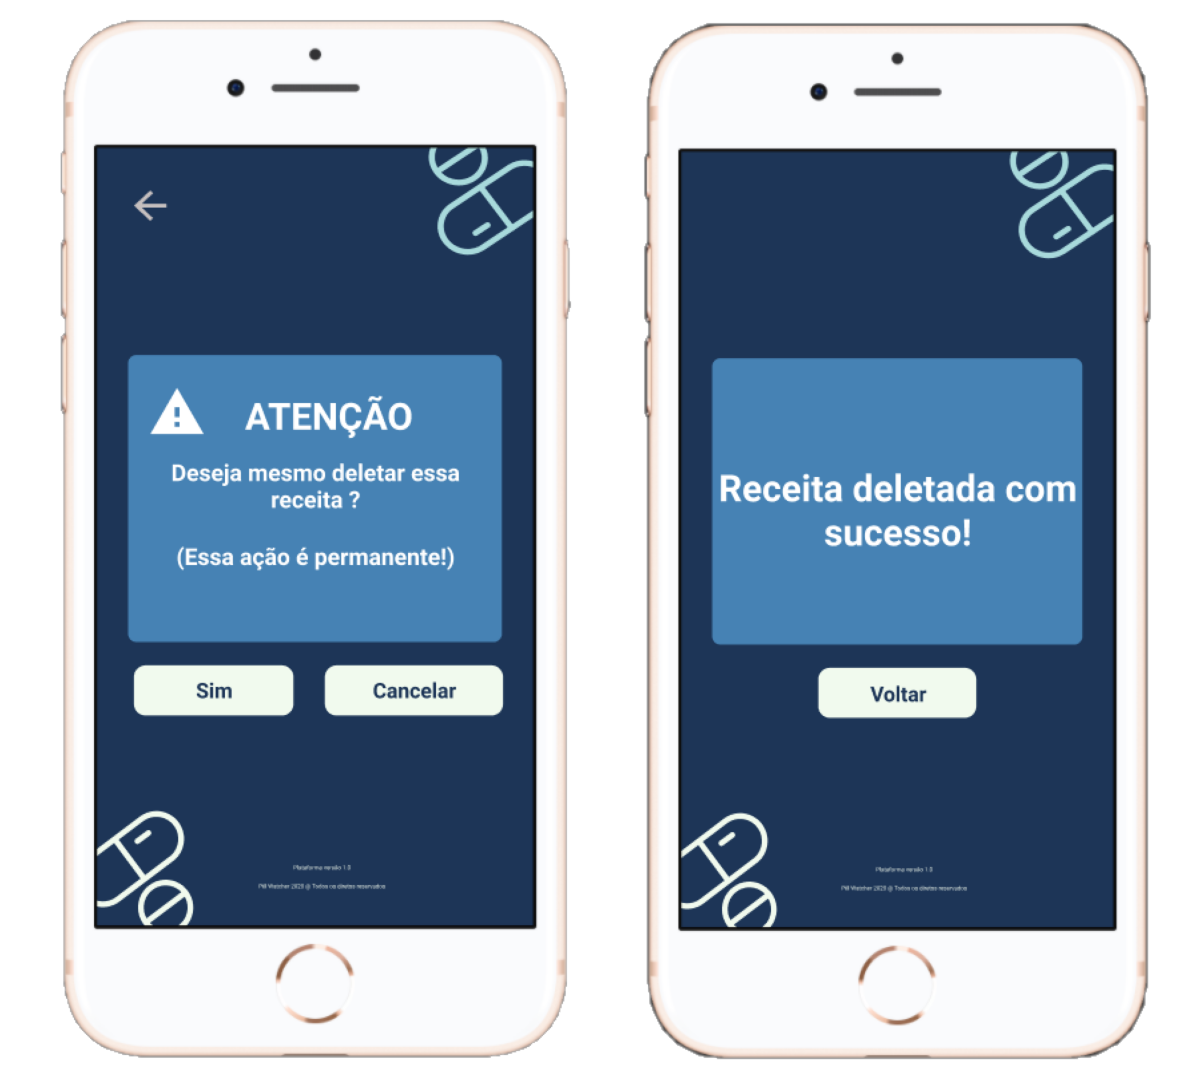
\includegraphics[width=8cm]{figuras/software/Atual_prototipo/Enfermeiro_gerenciarReceita_3.png}
     \label{fig:prototipo_enfermeiro_gerenciarReceita_3}}
    \subfloat[][Parte 1 do fluxo para cadastrar uma receita]{
    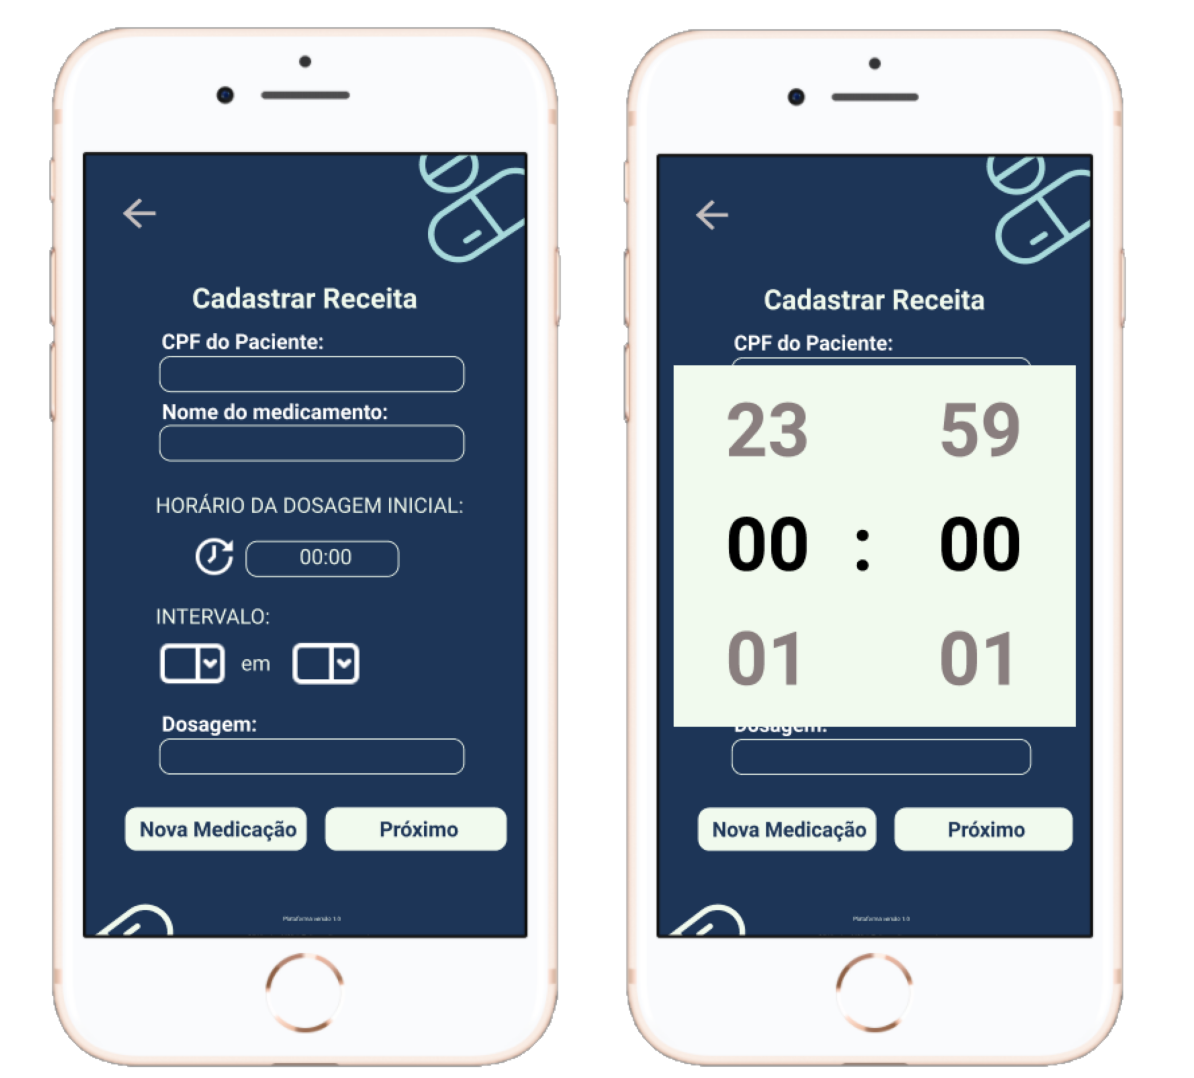
\includegraphics[width=8cm]{figuras/software/Atual_prototipo/Enfermeiro_gerenciarReceita_4.png}
    \label{fig:prototipo_enfermeiro_gerenciarReceita_4}}
    \caption{Enfermeiro - Fluxo para deletar receita e fluxo de cadastro de receita}
\end{figure}

Nas Fig. \ref{fig:prototipo_enfermeiro_gerenciarReceita_5} e \ref{fig:prototipo_enfermeiro_gerenciarReceita_6}, são mostradas as quatro telas finais para o cadastrado da receita, nas quais, é possível inserir observações, anexar uma foto da receita e concluir o cadastro recebendo o respectivo \textit{feedback}.

\begin{figure}[H]
    \centering
    \subfloat[][Parte 2 do fluxo para cadastrar uma receita]{
    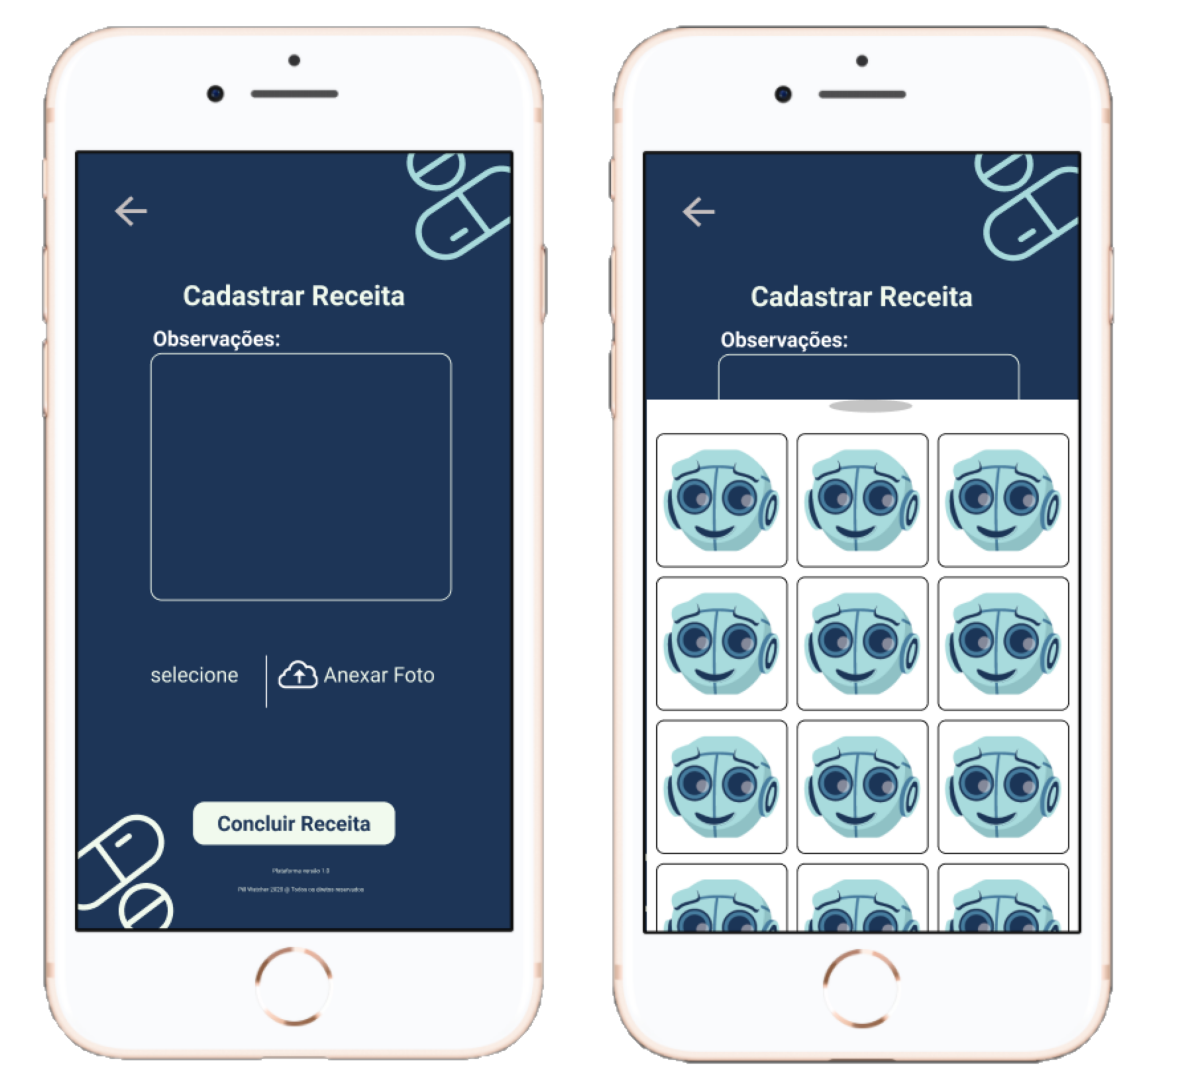
\includegraphics[width=8cm]{figuras/software/Atual_prototipo/Enfermeiro_gerenciarReceita_5.png}
     \label{fig:prototipo_enfermeiro_gerenciarReceita_5}}
    \subfloat[][Parte 3 do fluxo para cadastrar uma receita]{
    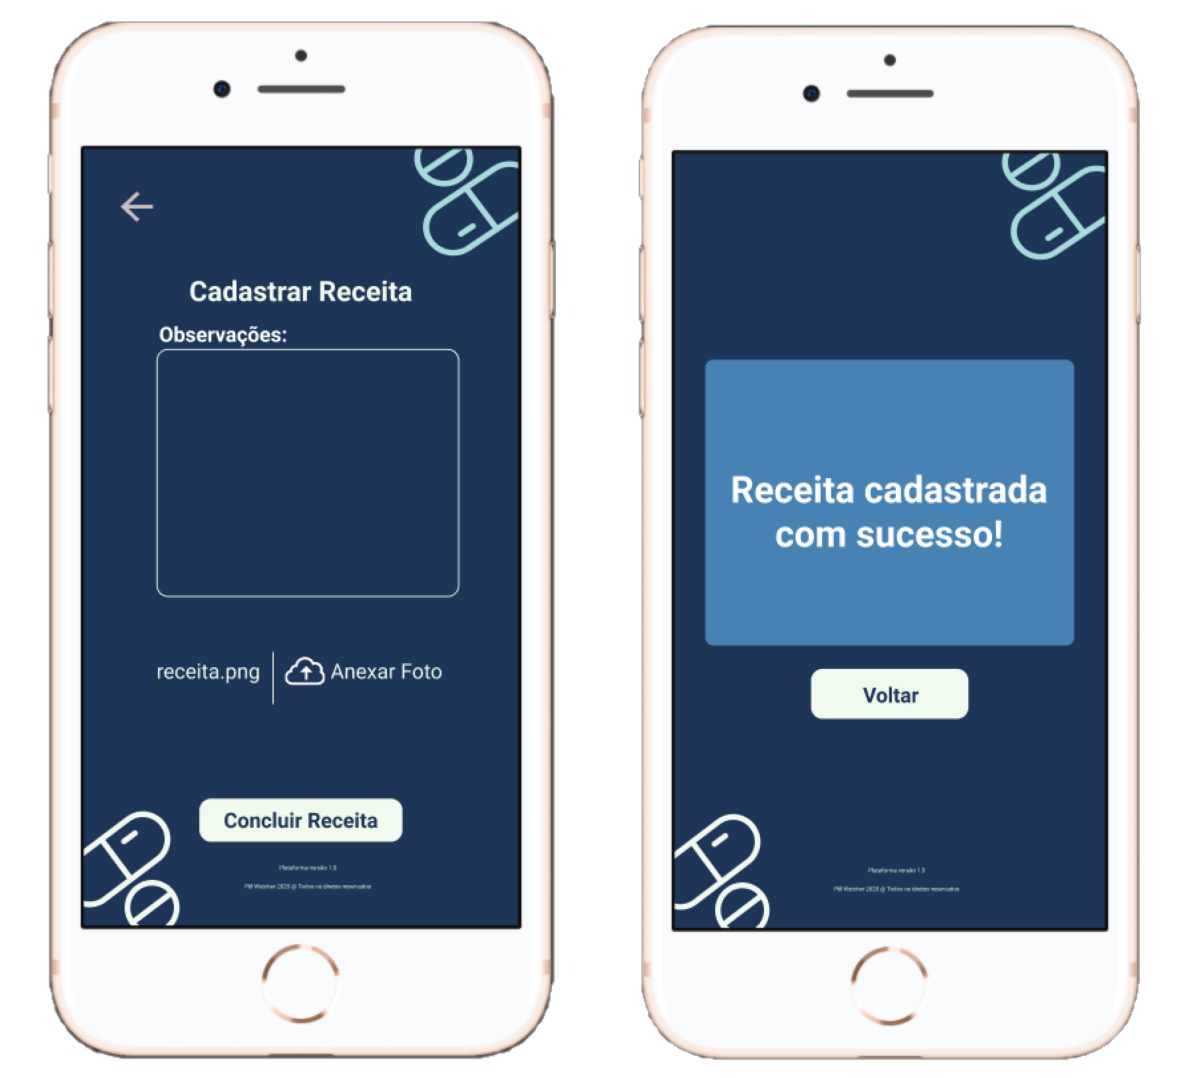
\includegraphics[width=8cm]{figuras/software/Atual_prototipo/Enfermeiro_gerenciarReceita_6.png}
    \label{fig:prototipo_enfermeiro_gerenciarReceita_6}}
    \caption{Enfermeiro - Fluxo de cadastro de receita}
\end{figure}

\begin{table}[H]
    \centering
    \caption{Tabela de Interações das Telas de Gerenciamento de Receita}
    \label{tab:interacao-telas-gerenciar-receita}
    \begin{adjustbox}{max width = \textwidth}
    % \begin{adjustwidth}{-2,5cm}{}
        \begin{tabular}{|L{4cm}|L{6cm}|L{4cm}|L{4cm}|L{3cm}|}
            \hline
            \rowcolor[HTML]{A8DADC}
            \multicolumn{1}{|c|}{\textbf{Tela}} & \multicolumn{1}{c|}{\textbf{Entrada}} & \multicolumn{1}{c|}{\textbf{Interações}} & \multicolumn{1}{c|}{\textbf{Saída}} & \multicolumn{1}{c|}{\textbf{Alternativo}} \\ \hline
             Tela de receitas cadastradas & Botão de gerenciamento de receita da tela principal do Enfermeiro & Filtrar por paciente, visualizar, editar, deletar ou cadastrar uma receita & Ícone de Retornar  & \multicolumn{1}{c|}{---} \\ \hline
             Tela de visualização de receita & Botão de visualizar receita da tela de gerenciamento de receita & \multicolumn{1}{c|}{---} & Ícone de Retornar & \multicolumn{1}{c|}{---} \\ \hline
             Tela de alteração de dados da receita & Botão de editar dados da receita da tela de gerenciamento de receita & Editar dados cadastrais da receita & Botão Salvar & Botão Voltar que direciona para tela de gerenciamento de receita\\ \hline
             Tela de \textit{feedback} da alteração de dados da receita & Botão de Salvar da tela de editar dados da receita & \multicolumn{1}{c|}{---} & Botão de fechar notificação & \multicolumn{1}{c|}{---} \\ \hline
             Tela de excluir receita cadastrada & Botão de excluir da tela de gerenciamento de receita & Clicar em `Sim' ou `Cancelar' & Botão `Sim' & Ao clicar em `Cancelar' ou `Voltar' o usuário é redirecionado a tela anterior \\ \hline
             Tela de cadastrar receita & Botão de `+' da tela de gerenciamento de receita & Adicionar dados cadastrais da receita & Botão `Concluir receita' & Ao clicar em `Voltar' o usuário é redirecionado a tela inicial de gerenciamento de receita \\ \hline
             Tela de \textit{feedback} de cadastro de receita & Botão de 'Concluir receita' da tela de cadastrar receita & \multicolumn{1}{c|}{---} & Clicar em `Voltar' & Botão `Voltar' que irá direcionar para tela inicial de gerenciamento de receita \\ \hline
             
        \end{tabular}
    % \end{adjustwidth}
    \end{adjustbox}
\end{table}

% \subsubsubsection{Gerenciar estoque da máquina}
\subparagraph*{} $-$ Gerenciar estoque da máquina

Na Fig. \ref{fig:prototipo_enfermeiro_gerenciarEstoqueMaquina_1} é mostrado a tela inicial do gerenciamento do estoque de medicamento da máquina e a busca filtrada por medicação. A Fig. \ref{fig:prototipo_enfermeiro_gerenciarEstoqueMaquina_2} é exibido o fluxo para deletar uma medicação do estoque da máquina.

\begin{figure}[H]
    \centering
    \subfloat[][Menu inicial de gerência de estoque da máquina \\ e busca por um medicamento]{
    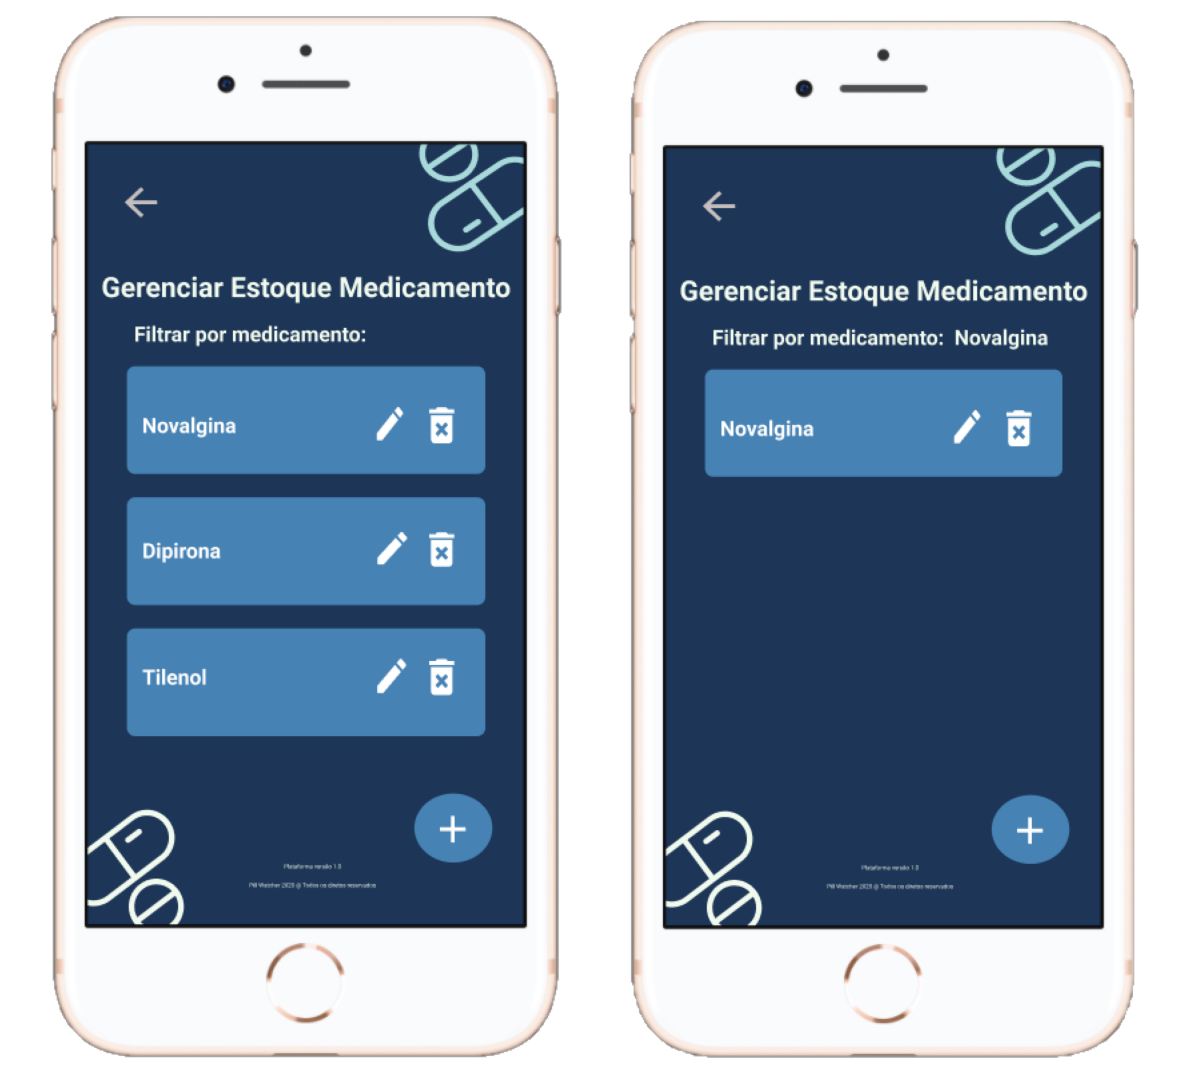
\includegraphics[width=8cm]{figuras/software/Atual_prototipo/Enfermeiro_gerenciarEstoqueMaquina_1.png}
     \label{fig:prototipo_enfermeiro_gerenciarEstoqueMaquina_1}}
    \subfloat[][Fluxo para deletar uma medicação do estoque da máquina]{
    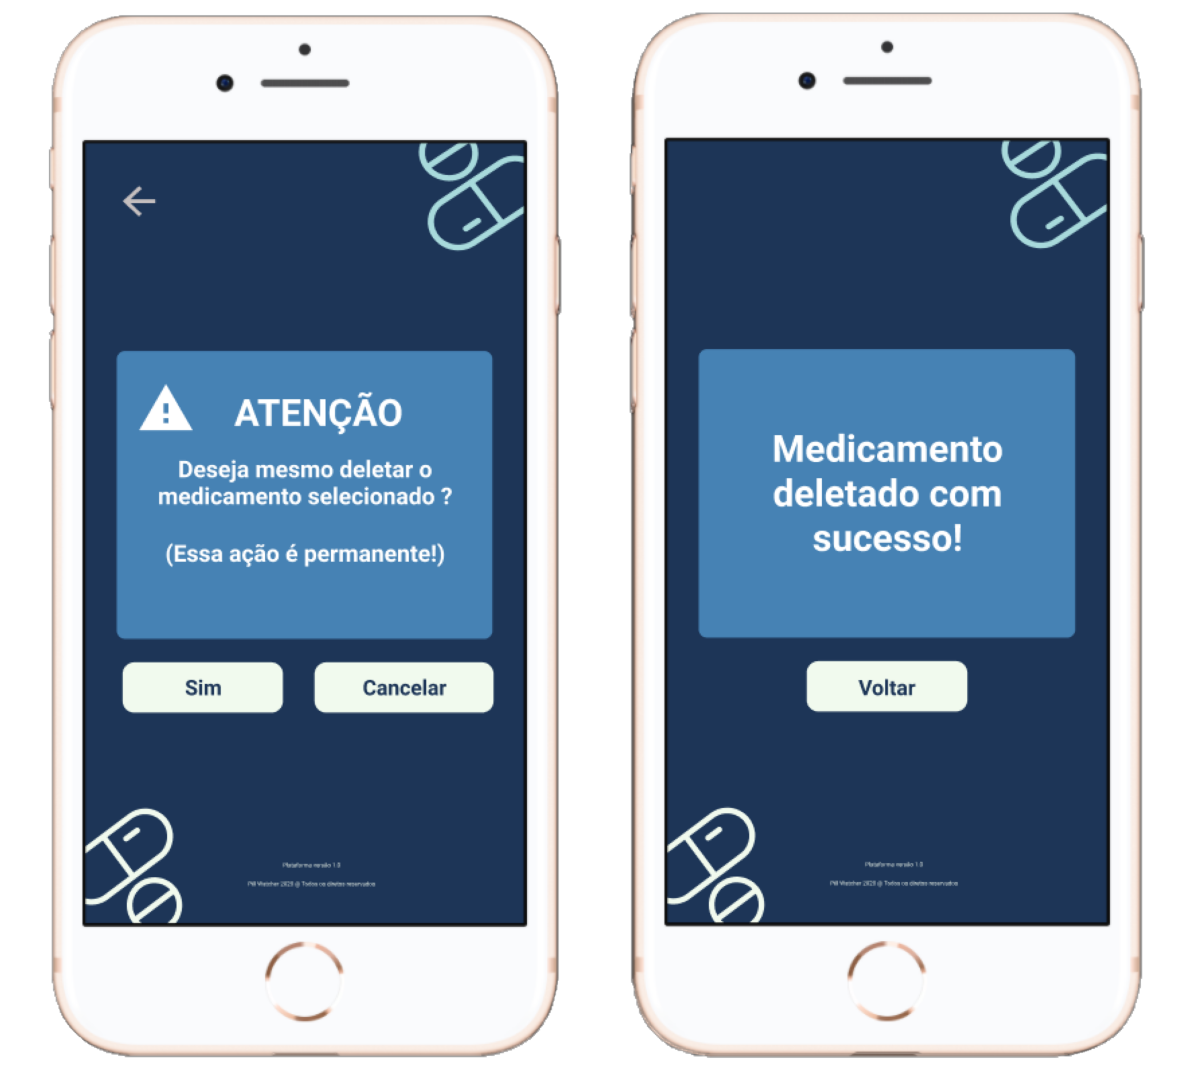
\includegraphics[width=8cm]{figuras/software/Atual_prototipo/Enfermeiro_gerenciarEstoqueMaquina_2.png}
    \label{fig:prototipo_enfermeiro_gerenciarEstoqueMaquina_2}}
    \caption{Enfermeiro - Menu inicial e fluxo para deletar medicação do estoque da máquina}
\end{figure}

A Fig. \ref{fig:prototipo_enfermeiro_gerenciarEstoqueMaquina_3} expõe o fluxo para alterar dados do estoque da máquina e seu respectivo \textit{feedback}.

\begin{figure}[H]
    \centering
      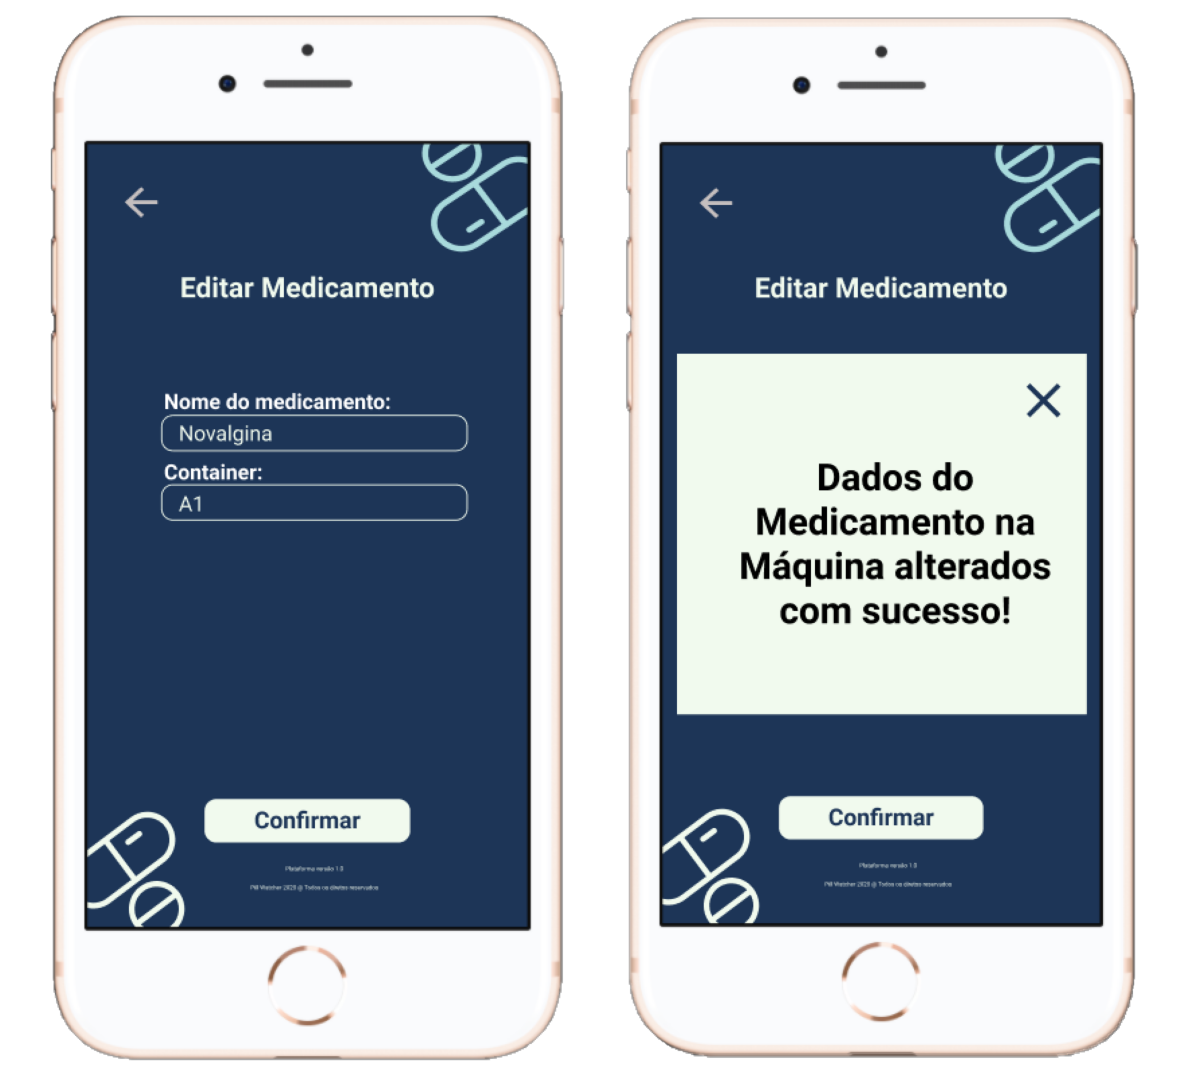
\includegraphics[width=10cm]{figuras/software/Atual_prototipo/Enfermeiro_gerenciarEstoqueMaquina_3.png}
    \caption{Enfermeiro - Fluxo para alterar dados do estoque da máquina}
    \label{fig:prototipo_enfermeiro_gerenciarEstoqueMaquina_3}
\end{figure}

Na Fig. \ref{fig:prototipo_enfermeiro_gerenciarEstoqueMaquina_4} denota o fluxo para cadastrar uma medicação no estoque da máquina.

\begin{figure}[H]
    \centering
      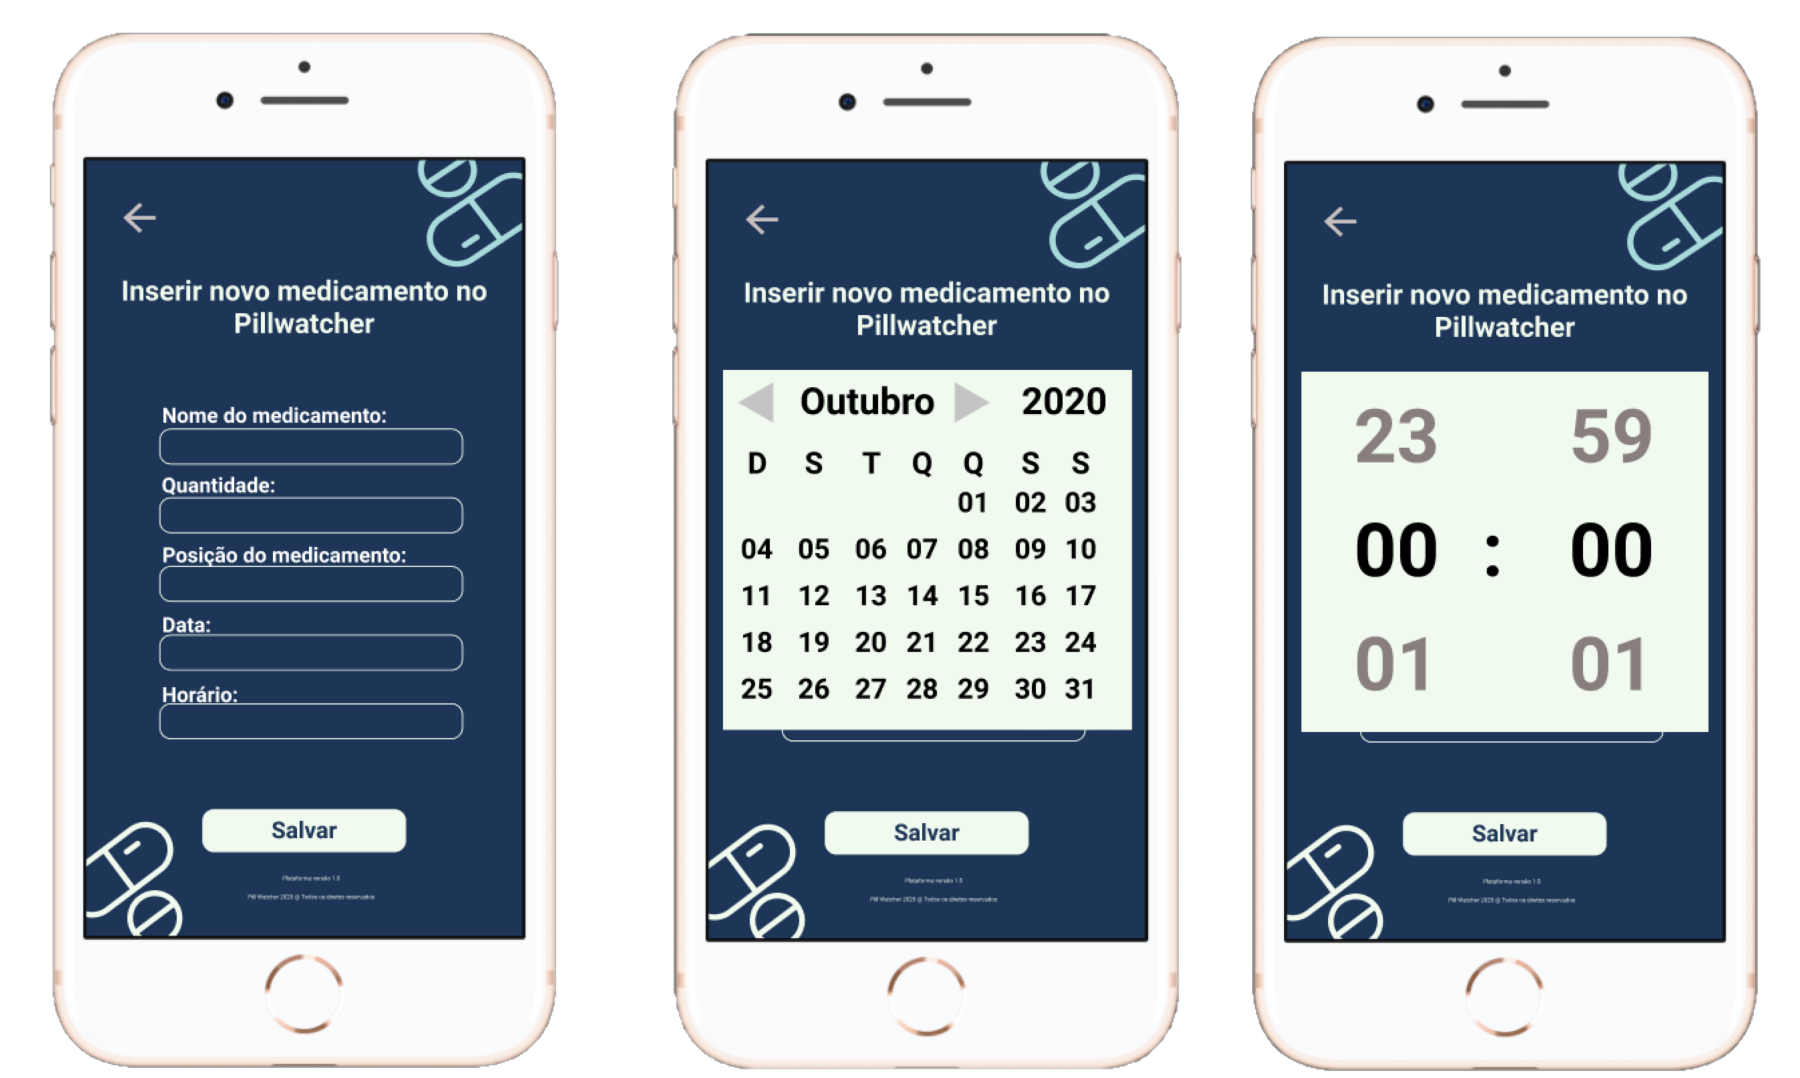
\includegraphics[width=15cm]{figuras/software/Atual_prototipo/Enfermeiro_gerenciarEstoqueMaquina_4.png}
    \caption{Enfermeiro - Fluxo para cadastrar uma medicação no estoque da máquina}
    \label{fig:prototipo_enfermeiro_gerenciarEstoqueMaquina_4}
\end{figure}

\begin{table}[H]
    \centering
    \caption{Tabela de interações das telas de gerenciamento de estoque da máquina}
    \label{tab:interacao-telas-notificacao_estoque}
    \begin{adjustbox}{max width = \textwidth}
    % \begin{adjustwidth}{-2,5cm}{}
        \begin{tabular}{|L{5cm}|L{4cm}|L{6cm}|L{4cm}|L{4cm}|}
            \hline
            \rowcolor[HTML]{A8DADC}
            \multicolumn{1}{|c|}{\textbf{Tela}} & \multicolumn{1}{c|}{\textbf{Entrada}} & \multicolumn{1}{c|}{\textbf{Interações}} & \multicolumn{1}{c|}{\textbf{Saída}} & \multicolumn{1}{c|}{\textbf{Alternativo}} \\ \hline
            Tela inicial de gerenciamento de estoque de medicamento da máquina & Botão `Gerenciar Estoque Máquina' do menu inicial do enfermeiro & Filtrar por medicamento, alterar dados do estoque, deletar e cadastrar um estoque da máquina & Botão 'Filtrar por medicamento', `Alterar', `Deletar' ou `Cadastrar' & Botão `Voltar' que irá direcionar ao menu inicial do enfermeiro \\ \hline
            Tela para deletar medicação do estoque da máquina & Botão `Deletar' da tela inicial de gerenciamento de estoque de medicamento & Confirmar a ação através do botão `Sim' e cancelar a ação por meio do botão `Cancelar' & Botão `Sim' ou `Cancelar' & Botão `Voltar' que irá direcionar à tela inicial de gerenciamento de estoque de medicamento da máquina \\ \hline
            Tela de \textit{feedback} de exclusão de medicamento do estoque da máquina & Botão `Sim' da tela para deletar medicação do estoque da máquina & Voltar para tela inicial de gerenciamento de estoque de medicamento da máquina & Botão `Voltar' que irá direcionar à tela inicial de gerenciamento de estoque de medicamento da máquina & \multicolumn{1}{c|}{---} \\ 
            \hline
            Tela de alteração dos dados de um medicamento do estoque da máquina & Botão `Alterar' da tela inicial de gerenciamento de estoque de medicamento da máquina & Alterar dados cadastrados de um medicamento do estoque da máquina & Botão `Confirmar' & Botão `Voltar' que irá direcionar à tela inicial de gerenciamento de estoque de medicamento da máquina \\ \hline
            Tela de \textit{feedback} de alteração dos dados de um medicamento do estoque da máquina & Botão `Confirmar' da tela de alteração dos dados de um medicamento do estoque da máquina & Fechar \textit{feedback} & Botão `X' & \multicolumn{1}{c|}{---} \\ 
            \hline
            Tela para inserção de novo medicamento no estoque da máquina & Botão `+' da tela inicial de gerenciamento de estoque de medicamento da máquina & Preenchimento de dados cadastrais do medicamento a ser inserido no estoque da máquina & Botão `Salvar' & Botão `Voltar' que irá direcionar à tela inicial de gerenciamento de estoque de medicamento da máquina \\ 
            \hline
        \end{tabular}
    % \end{adjustwidth}
    \end{adjustbox}
\end{table}

% \subsubsubsection{Abastecer Pillwatcher}
\subparagraph*{} $-$ Abastecer \textit{Pillwatcher}

Para abastecer o \textit{Pillwatcher}, o primeiro passo é o gerenciamento de estoque por paciente, ilustrado pela Fig. \ref{fig:prototipo_enfermeiro_abastecer_1} que demonstra a tela inicial de gerenciamento de estoque, em seguida, a busca filtrada por paciente. A Fig. \ref{fig:prototipo_enfermeiro_abastecer_1-1} aponta a visualização mais detalhada do estoque individual e a tela para cadastro de um estoque individual. 

\begin{figure}[H]
     \centering
    \subfloat[][Tela inicial de gerenciar estoque e busca filtrada por paciente]{
    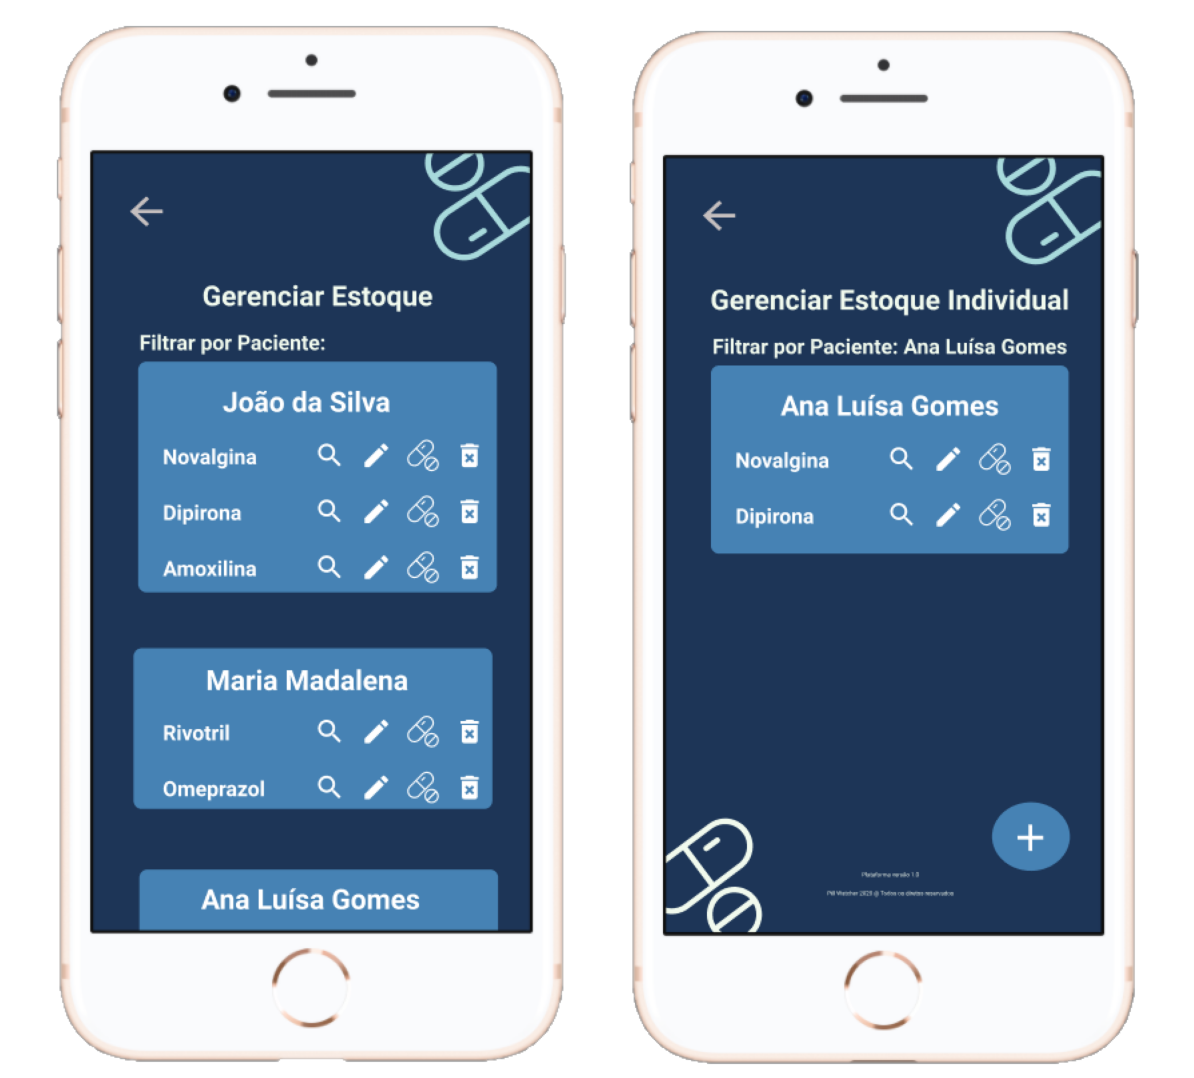
\includegraphics[width=8cm]{figuras/software/Atual_prototipo/Enfermeiro_abastecer_1.png}
     \label{fig:prototipo_enfermeiro_abastecer_1}}
    \subfloat[][Visualização do estoque de determinada medicação e tela para cadastro de estoque]{
    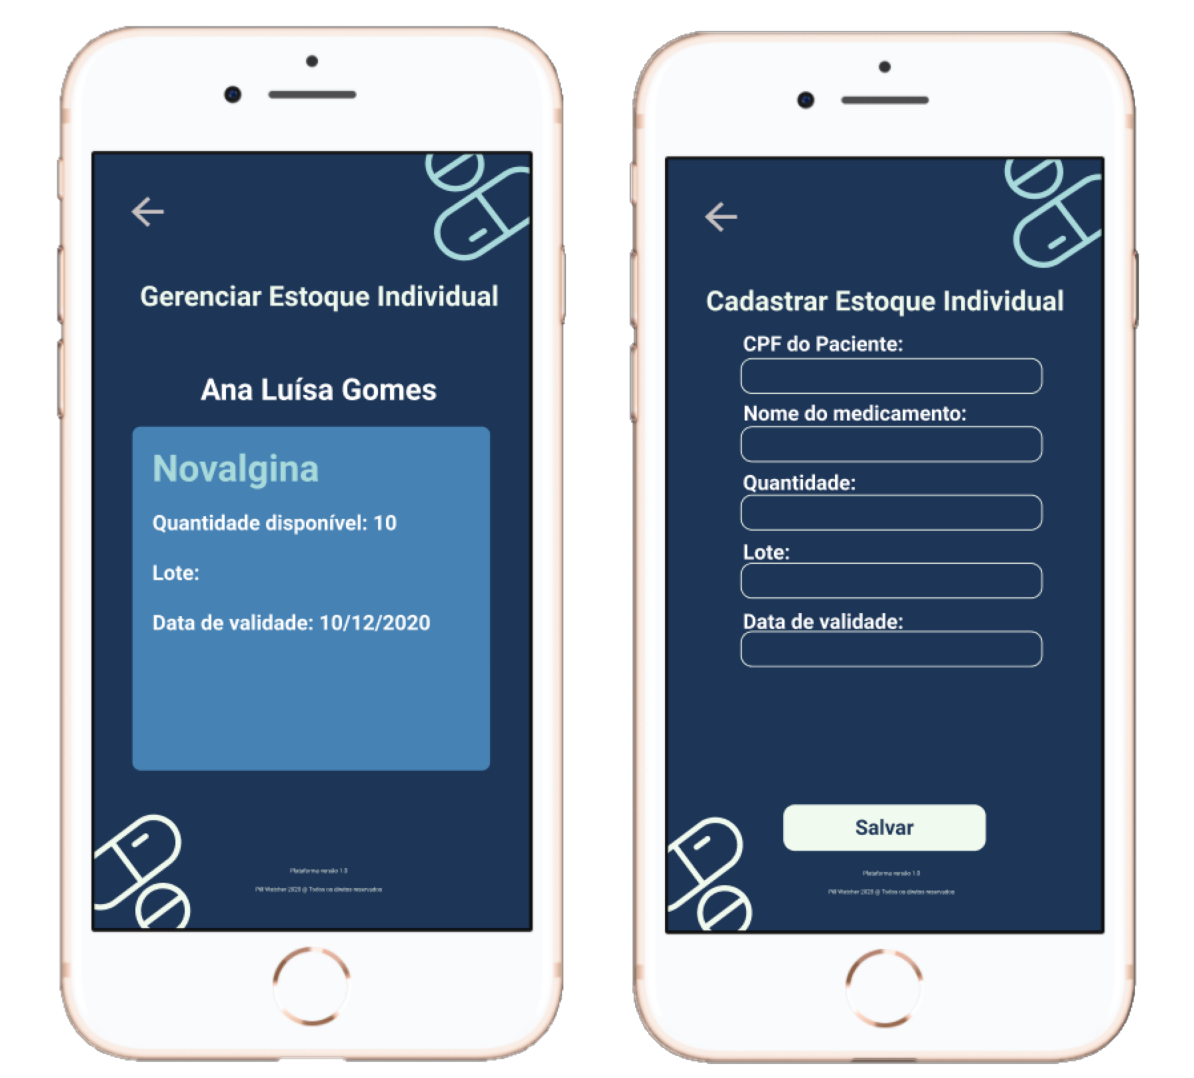
\includegraphics[width=8cm]{figuras/software/Atual_prototipo/Enfermeiro_abastecer_1-1.png}
    \label{fig:prototipo_enfermeiro_abastecer_1-1}}
    \caption{Enfermeiro - Menu inicial, visualização e cadastro de estoque individual}
\end{figure}

A Fig. \ref{fig:prototipo_enfermeiro_abastecer_2} demonstra o fluxo de alteração de dados acerca do estoque individual de determinado remédio e paciente, além do respectivo \textit{feedback} relacionado a essa ação.

\begin{figure}[H]
    \centering
    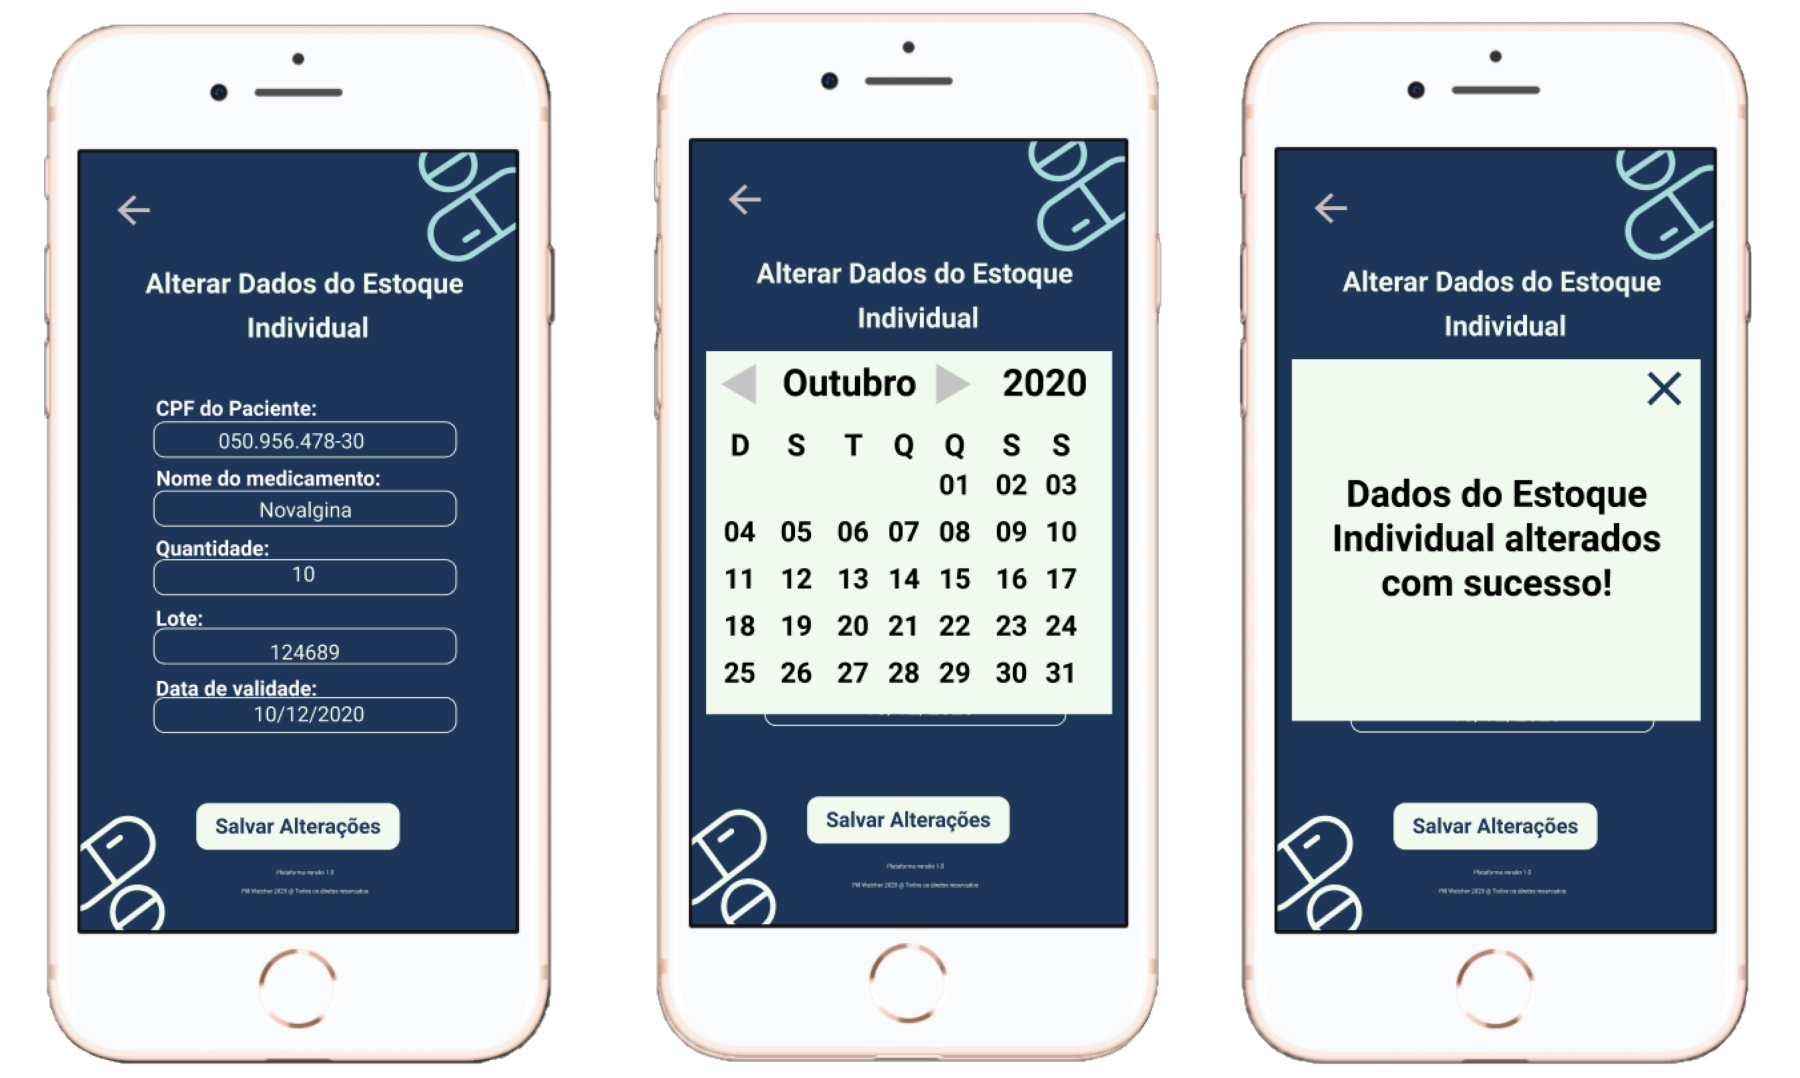
\includegraphics[width=15cm]{figuras/software/Atual_prototipo/Enfermeiro_abastecer_2.png}
    \caption{Enfermeiro - Fluxo de alteração de dados de um estoque individual}
    \label{fig:prototipo_enfermeiro_abastecer_2}
\end{figure}

As Fig. \ref{fig:prototipo_enfermeiro_abastecer_3} e \ref{fig:prototipo_enfermeiro_abastecer_4} exibem o fluxo de abastecimento após ser selecionado o paciente e o medicamento em fluxo apresentado previamente (Fig. \ref{fig:prototipo_enfermeiro_abastecer_1}).

\begin{figure}[H]
    \centering
    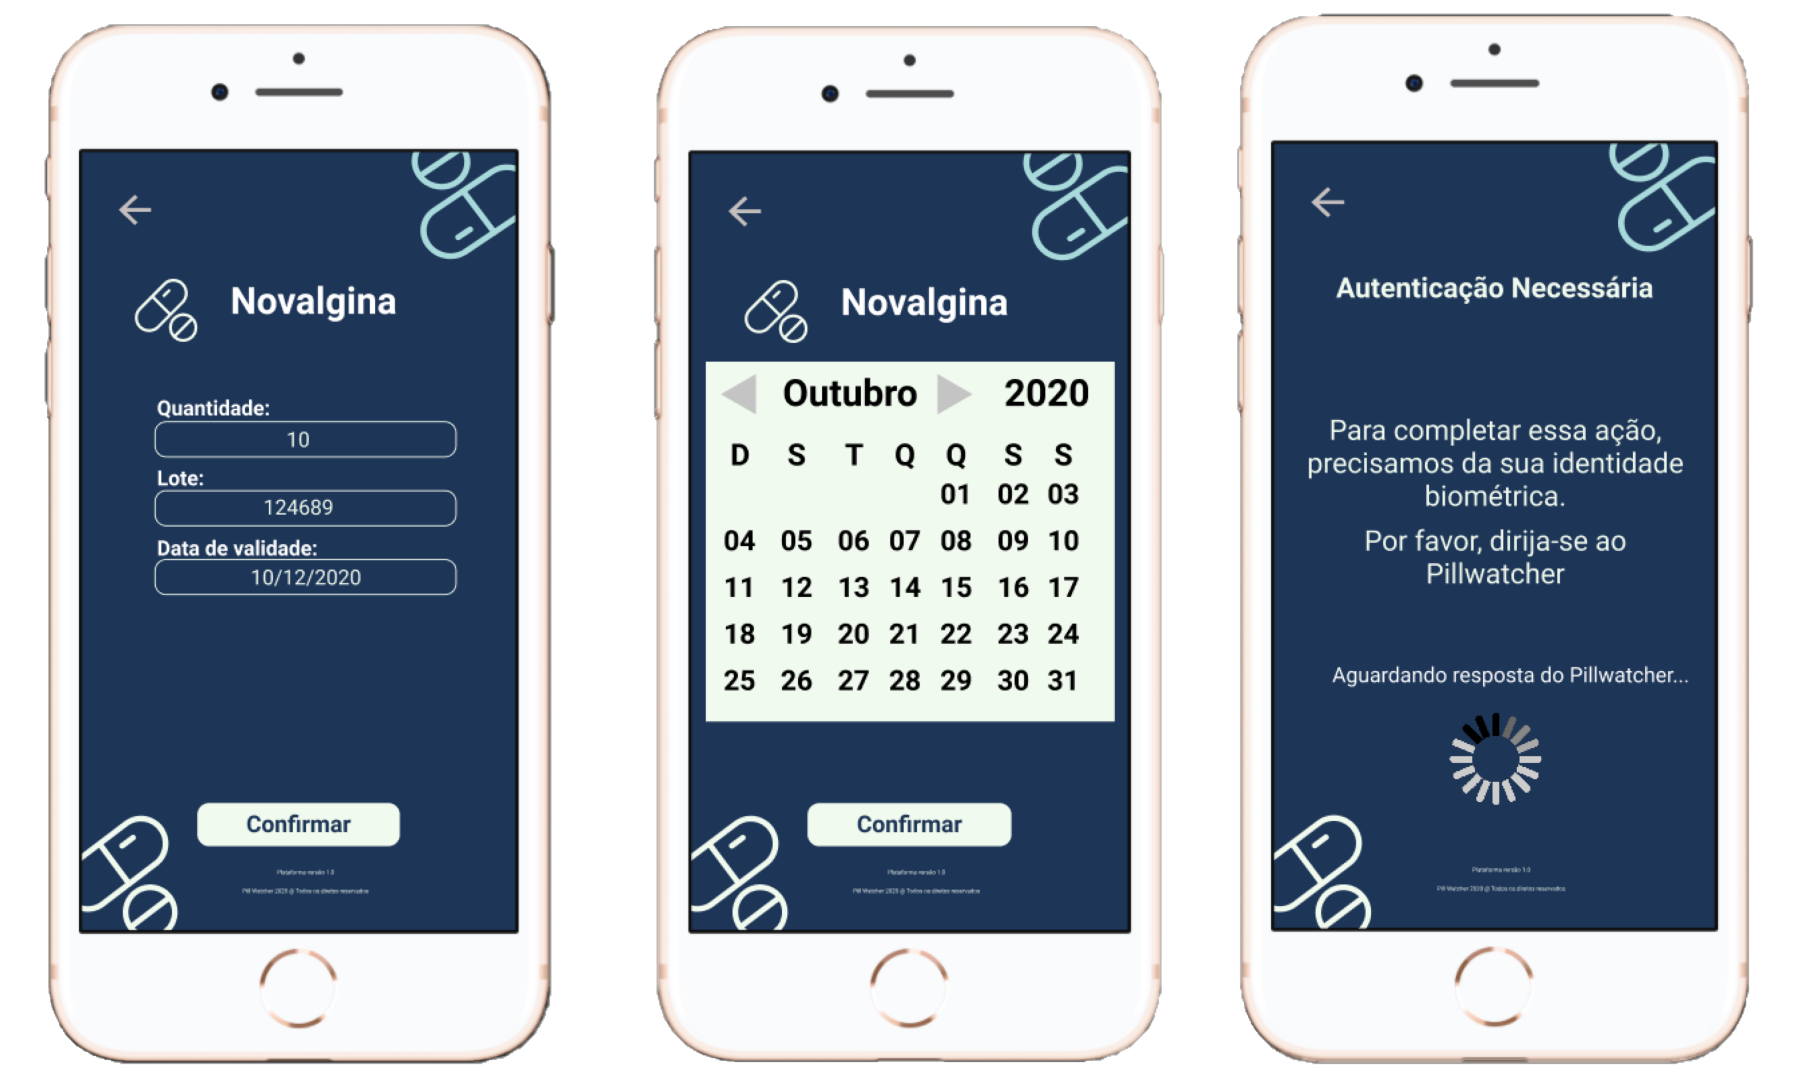
\includegraphics[width=15cm]{figuras/software/Atual_prototipo/Enfermeiro_abastecer_3.png}
    \caption{Enfermeiro - Parte 1 do fluxo de abastecimento de uma medicação}
    \label{fig:prototipo_enfermeiro_abastecer_3}
\end{figure}

\begin{figure}[H]
    \centering
    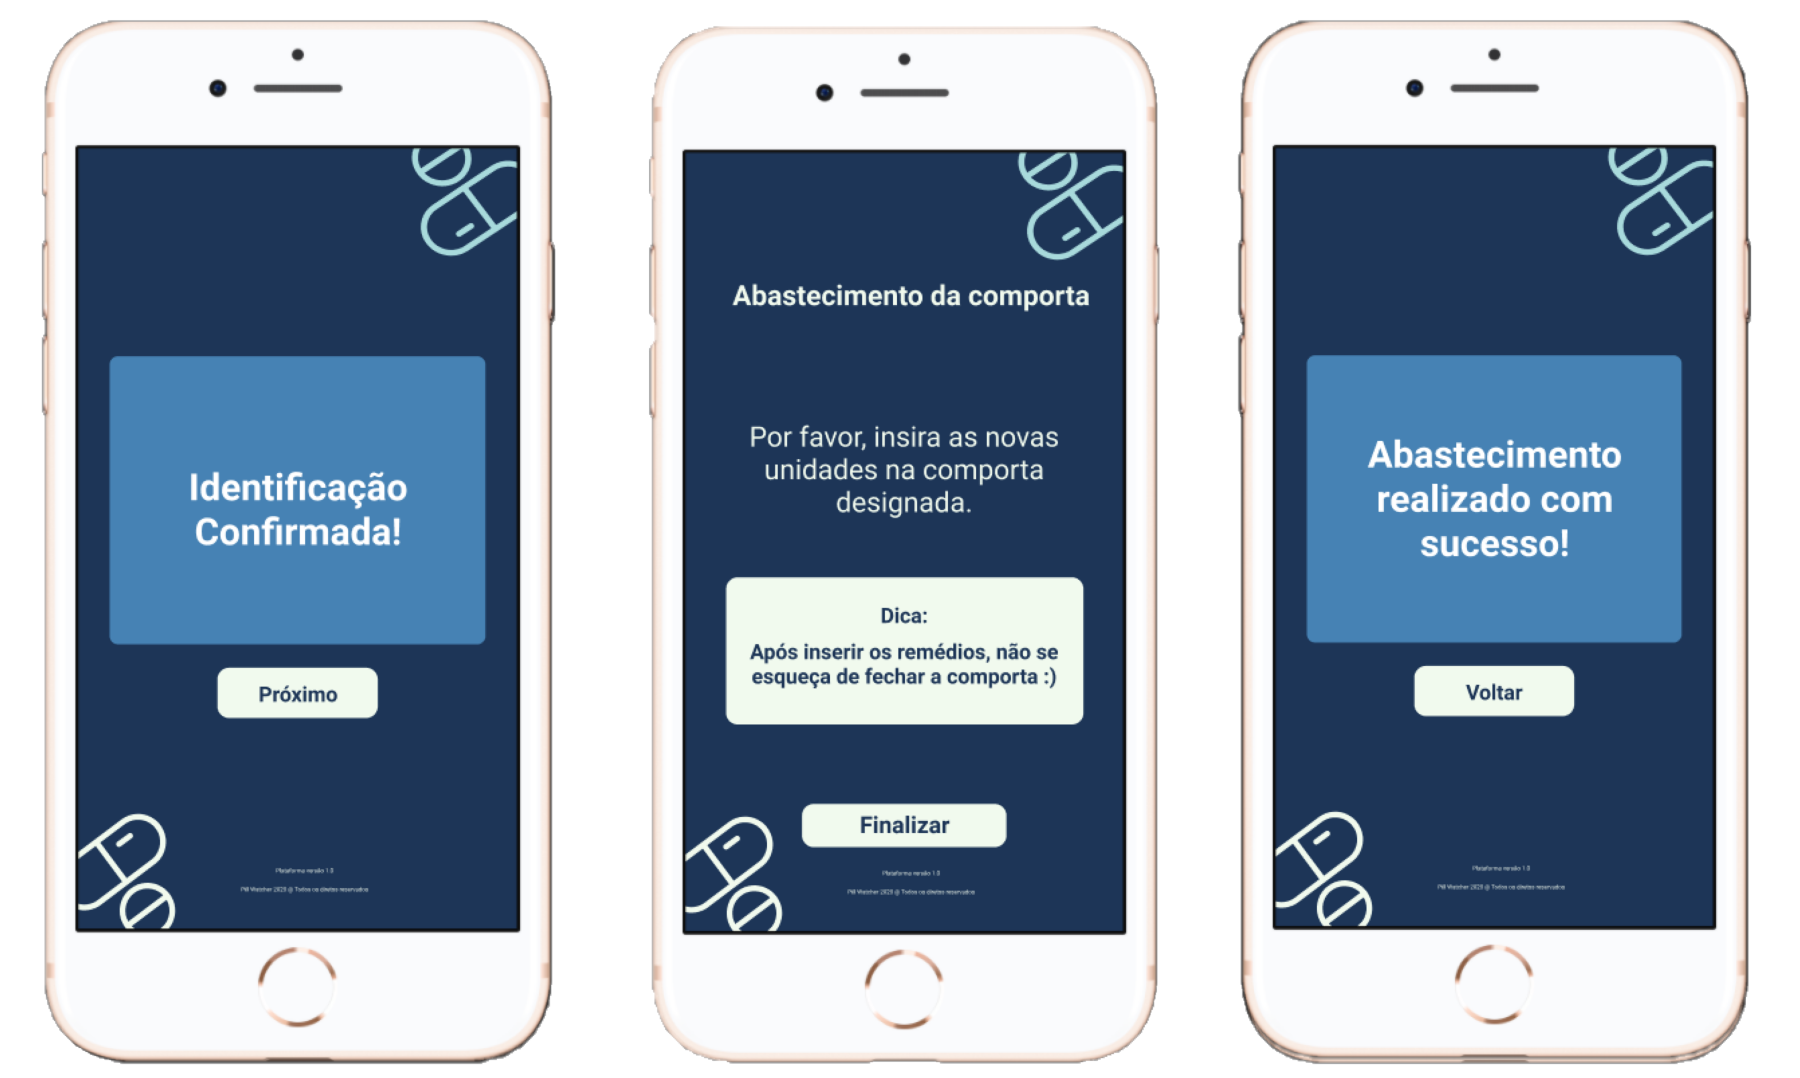
\includegraphics[width=15cm]{figuras/software/Atual_prototipo/Enfermeiro_abastecer_4.png}
    \caption{Enfermeiro - Parte 2 do fluxo de abastecimento de uma medicação}
    \label{fig:prototipo_enfermeiro_abastecer_4}
\end{figure}

A Fig. \ref{fig:prototipo_enfermeiro_abastecer_5} indica o fluxo para deletar uma medicação do estoque individual do paciente e o \textit{feedback} fornecido para essa ação.

\begin{figure}[H]
    \centering
    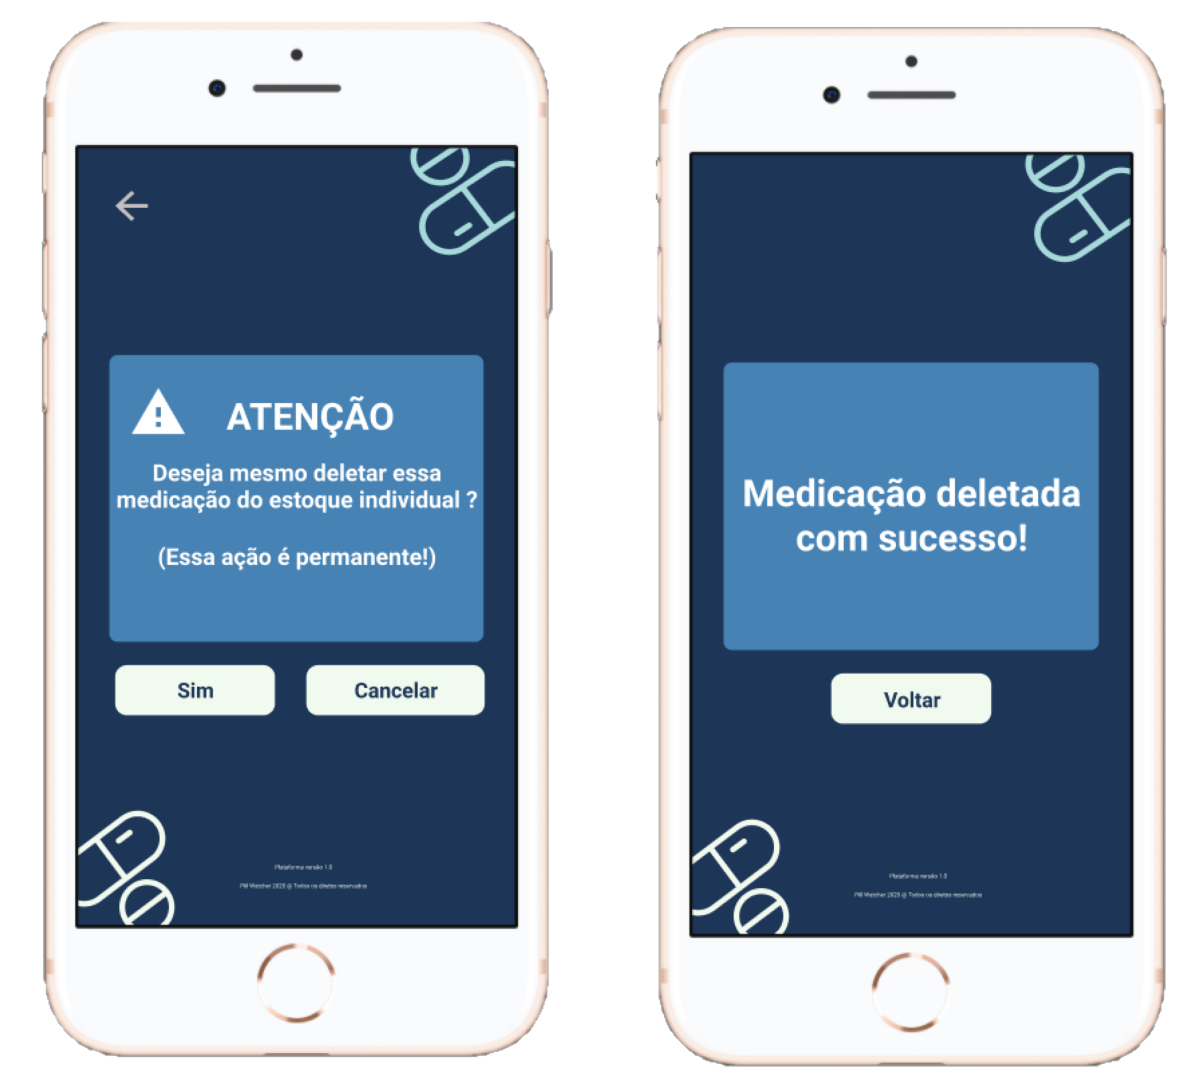
\includegraphics[width=10cm]{figuras/software/Atual_prototipo/Enfermeiro_abastecer_5.png}
    \caption{Enfermeiro - Fluxo para deletar uma medicação do estoque individual}
    \label{fig:prototipo_enfermeiro_abastecer_5}
\end{figure}

\begin{table}[H]
    \centering
    \caption{Tabela de interações das telas de abastecimento do \textit{Pillwatcher}}
    \label{tab:interacao-telas-abastecimento}
    \begin{adjustbox}{max width = \textwidth}
    % \begin{adjustwidth}{-2,5cm}{}
        \begin{tabular}{|L{5cm}|L{4cm}|L{6cm}|L{4cm}|L{4cm}|}
            \hline
            \rowcolor[HTML]{A8DADC}
            \multicolumn{1}{|c|}{\textbf{Tela}} & \multicolumn{1}{c|}{\textbf{Entrada}} & \multicolumn{1}{c|}{\textbf{Interações}} & \multicolumn{1}{c|}{\textbf{Saída}} & \multicolumn{1}{c|}{\textbf{Alternativo}} \\ \hline
             Tela de Gerenciar Estoque & Botão de Abastecer \textit{Pillwatcher} da tela principal do Enfermeiro & Filtrar por paciente, visualizar, editar, abastecer, deletar e cadastrar estoque individual & Botão `Visualizar', `Editar', `Abastecer', `Deletar' e `+' & \multicolumn{1}{c|}{---} \\ \hline
             Tela de visualizar estoque individual & Botão `Visualizar' da tela inicial de gerenciamento de estoque  & \multicolumn{1}{c|}{---}  & Botão `Voltar' que irá direcionar para tela inicial de gerenciamento de estoque & \multicolumn{1}{c|}{---} \\ \hline
             Tela de alteração de dados do estoque individual & Botão `Editar' da tela inicial de gerenciamento de estoque & Alterar dados cadastrais do estoque individual & Botão `Salvar alterações'  & Botão `Voltar' que irá direcionar para tela inicial de gerenciamento de estoque \\ \hline
             Tela de \textit{feedback} da alteração de dados do estoque individual & Botão `Salvar alterações' & Fechar \textit{feedback} & Botão `X' & \multicolumn{1}{c|}{---} \\ \hline
             Tela inicial de abastecimento de uma medicação & Botão `Abastecer' da tela inicial de gerenciamento de estoque & Inserção de quantidade, lote e data de validade & Botão `Confirmar'  & Botão `Voltar' que irá direcionar para tela inicial de gerenciamento de estoque \\ \hline
             Tela de autenticação para abastecimento de uma medicação & Botão `Confirmar' da tela inicial de abastecimento de uma medicação & Inserção de biometria no dispositivo do \textit{Pillwatcher} & Biometria confirmada  & \multicolumn{1}{c|}{---} \\ \hline
             Tela de \textit{feedback} de biometria confirmada & Biometria confirmada & Ir para o próximo passo & Botão `Próximo'  & \multicolumn{1}{c|}{---} \\ \hline
             Tela de abastecimento da comporta & Botão `Próximo' após a identidade ser confirmada & Finalizar o abastecimento & Botão 'Finalizar'  & \multicolumn{1}{c|}{---} \\ \hline
             Tela de \textit{feedback} de abastecimento & Botão `Finalizar' & Voltar para tela inicial de gerenciamento de estoque individual & Botão `Voltar' & \multicolumn{1}{c|}{---} \\ \hline
             Tela de deletar uma medicação do estoque individual & Botão `Deletar' da tela inicial de gerenciamento de estoque individual &  Confirmar a exclusão através do botão 'Sim' ou cancelar a ação através do `Cancelar'  & Botão 'Sim' ou `Cancelar' & Botão `Voltar' que irá direcionar para tela inicial de gerenciamento de estoque \\ \hline
             Tela de \textit{feedback} de exclusão de uma medicação do estoque individual & Botão `Sim' da tela de deletar uma medicação do estoque individual & Voltar para tela inicial de gerenciamento de estoque individual  & Botão `Voltar' & \multicolumn{1}{c|}{---} \\ \hline
             
        \end{tabular}
    % \end{adjustwidth}
    \end{adjustbox}
\end{table}

% \subsubsubsection{Notificação de entrega de medicação}
\subparagraph*{} $-$ Notificação de entrega de medicação

A Fig. \ref{fig:prototipo_enfermeiro_notificacao} denota a notificação que será recebida pelo enfermeiro minutos antes de uma medicação ser entregue e o respectivo \textit{feedback} exibido quando o enfermeiro confirma a entrega na tela anterior.

\begin{figure}[H]
    \centering
    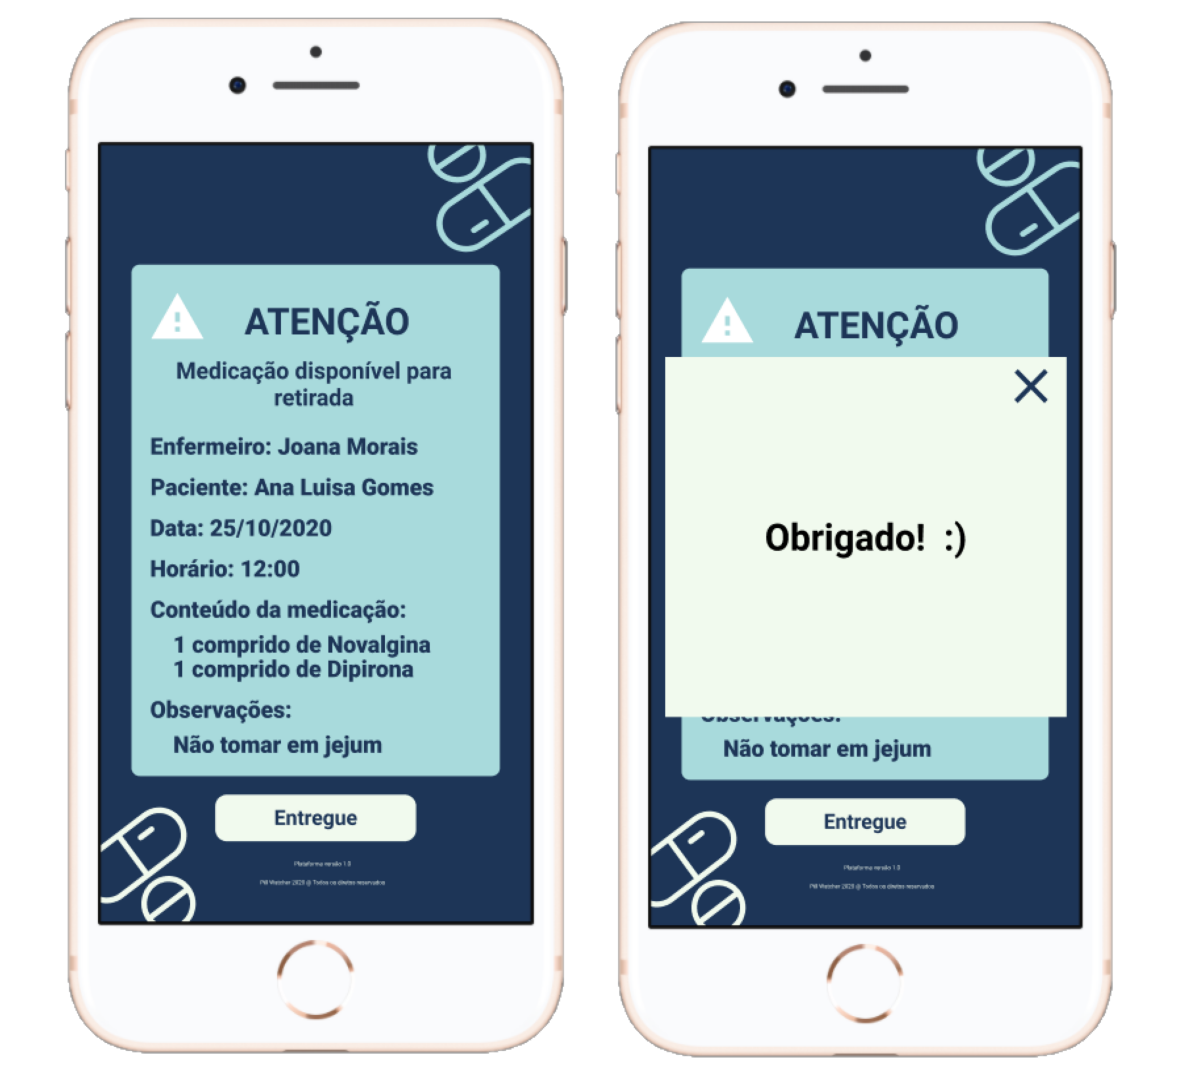
\includegraphics[width=12cm]{figuras/software/Atual_prototipo/Enfermeiro_notificacao.png}
    \caption{Enfermeiro - Fluxo de notificação do enfermeiro}
    \label{fig:prototipo_enfermeiro_notificacao}
\end{figure}

\begin{table}[H]
    \centering
    \caption{Tabela de interações das telas de notificação de entrega de medicação}
    \label{tab:interacao-telas-notificacao_medicacao}
    \begin{adjustbox}{max width = \textwidth}
    % \begin{adjustwidth}{-2,5cm}{}
        \begin{tabular}{|L{5cm}|L{6cm}|L{4cm}|c|c|}
            \hline
            \rowcolor[HTML]{A8DADC}
            \multicolumn{1}{|c|}{\textbf{Tela}} & \multicolumn{1}{c|}{\textbf{Entrada}} & \multicolumn{1}{c|}{\textbf{Interações}} & \multicolumn{1}{c|}{\textbf{Saída}} & \multicolumn{1}{c|}{\textbf{Alternativo}} \\ \hline
             Notificação de medicação a ser entregue & O dispositivo do \textit{Pillwatcher} dispara a notificação para o software minutos antes do horário da medicação & Confirmar entrega da medicação através do botão `Entregue'  & Botão `Entregue' & \multicolumn{1}{c|}{---} \\ \hline
              Tela de \textit{feedback} da entrega da medicação & Botão `Entregue' da tela anterior & Fechar \textit{feedback} & Botão `X' & \multicolumn{1}{c|}{---} \\ \hline
        \end{tabular}
    % \end{adjustwidth}
    \end{adjustbox}
\end{table}


% \subsubsection{Paciente}
\subparagraph*{$\bullet$ Paciente} \hfill
% \subsubsubsection{Menu Inicial e \textit{sidebar}}
\subparagraph*{} $-$ Menu Inicial e \textit{sidebar}

A Fig. \ref{fig:prototipo_paciente_menuSidebar_1} expõe o menu inicial do paciente, a barra lateral com seus respectivos dados cadastrados e a primeira tela do fluxo para alterar esses.

\begin{figure}[H]
    \centering
    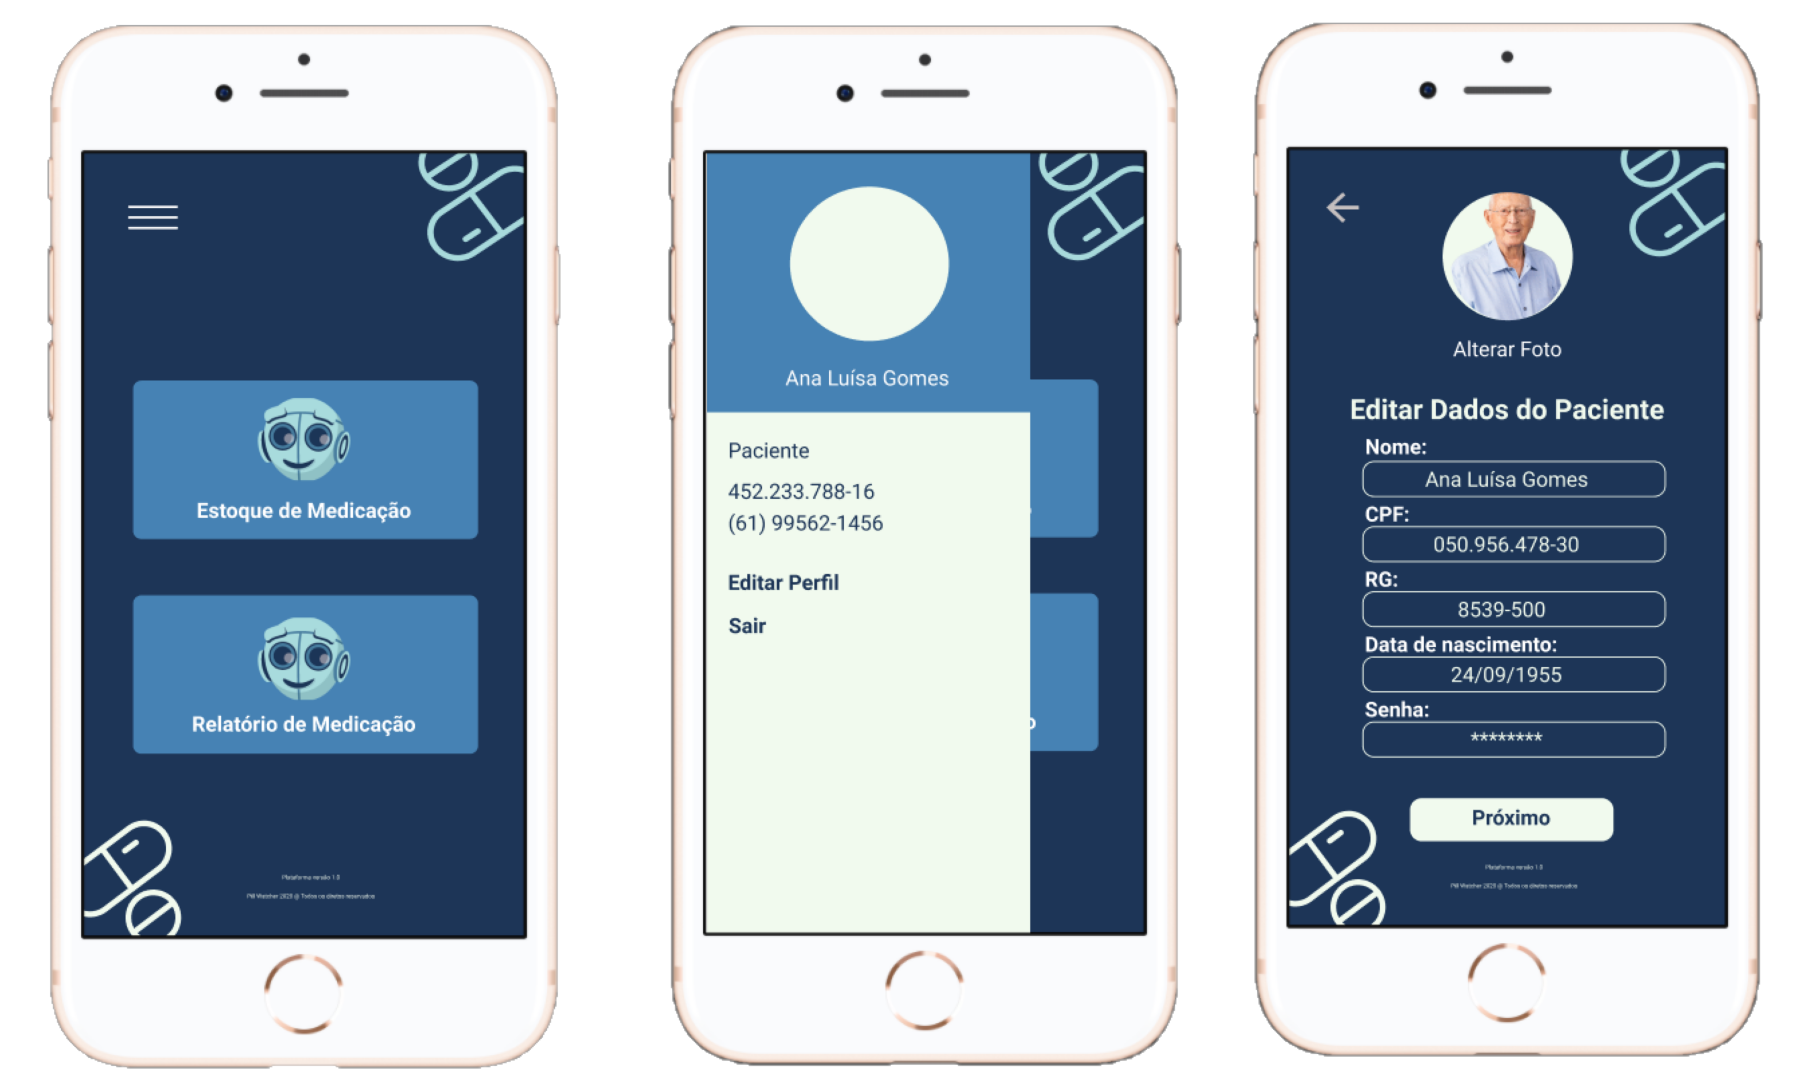
\includegraphics[width=15cm]{figuras/software/Atual_prototipo/Paciente_menuSidebar_1.png}
    \caption{Paciente - Menu inicial, \textit{sidebar} e Parte 1 do fluxo para alterar dados cadastrados}
    \label{fig:prototipo_paciente_menuSidebar_1}
\end{figure}

As Fig. \ref{fig:prototipo_paciente_menuSidebar_2} e \ref{fig:prototipo_paciente_menuSidebar_3} ilustram o fluxo para editar os dados cadastrados acerca do paciente e do familiar, e o \textit{feedback} para essa ação.

\begin{figure}[H]
    \centering
    \subfloat[][Parte 2 do fluxo para alterar dados cadastrados]{
    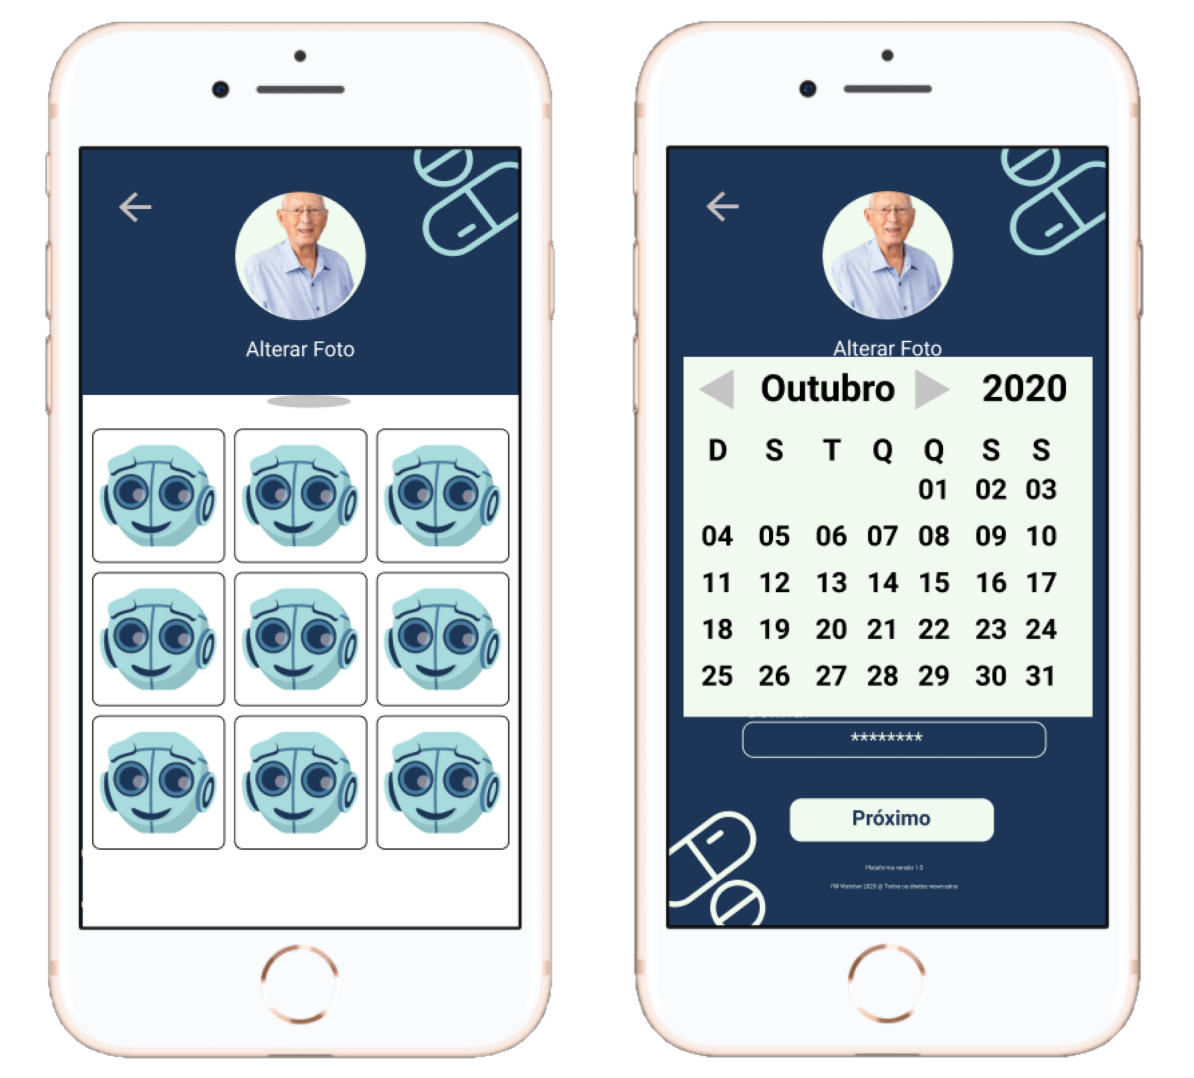
\includegraphics[width=8cm]{figuras/software/Atual_prototipo/Paciente_menuSidebar_2.png}
     \label{fig:prototipo_paciente_menuSidebar_2}}
    \subfloat[][Parte 3 do fluxo para alterar dados cadastrados]{
    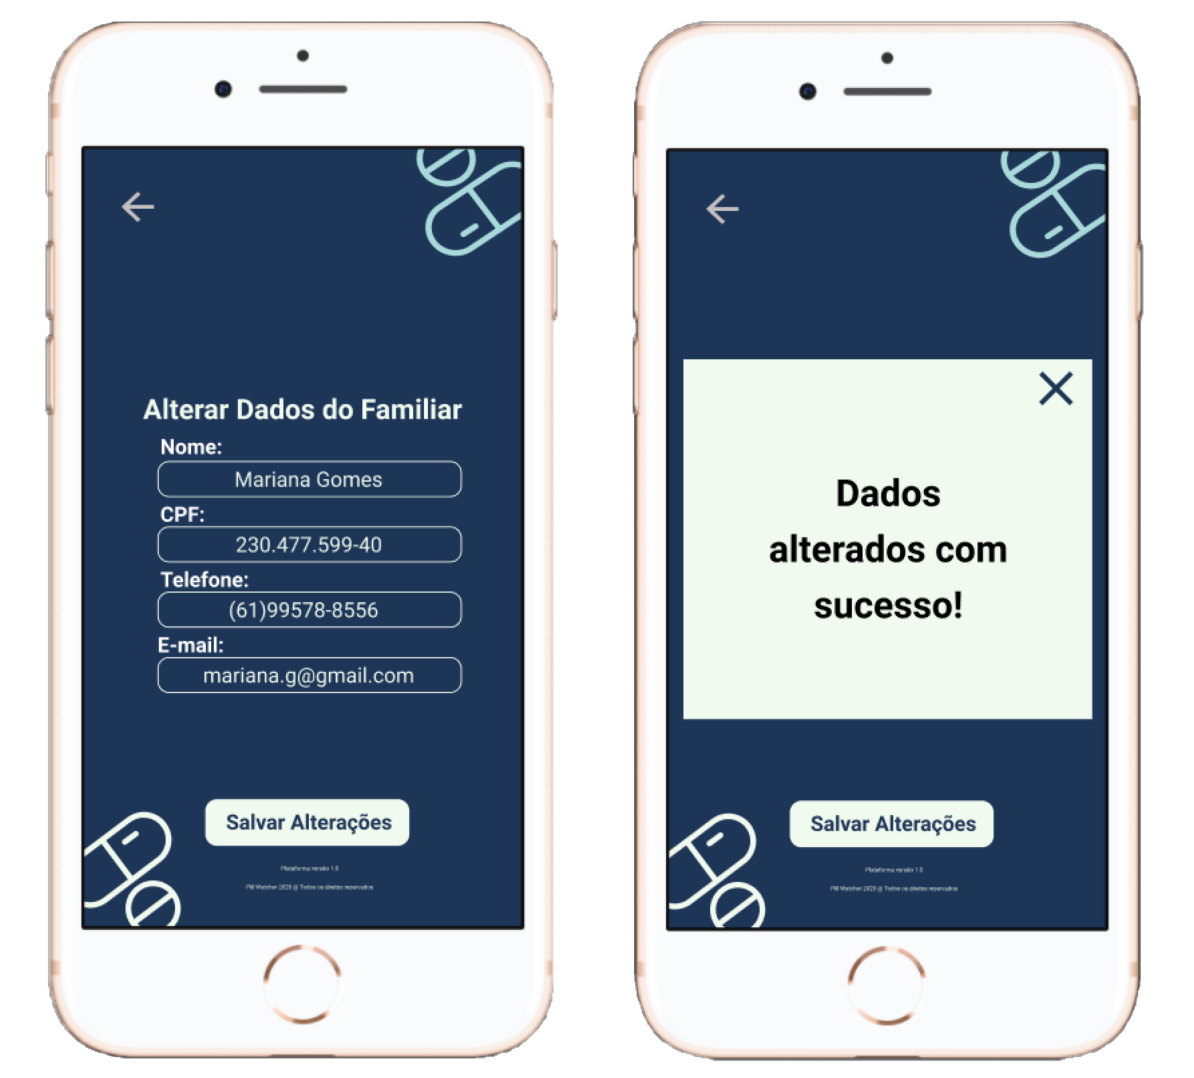
\includegraphics[width=8cm]{figuras/software/Atual_prototipo/Paciente_menuSidebar_3.png}
    \label{fig:prototipo_paciente_menuSidebar_3}}
    \caption{Paciente - Conclusão do fluxo para alterar dados cadastrados}
\end{figure}

\begin{table}[H]
    \centering
    \caption{Tabela de interações das telas de Menu inicial e \textit{sidebar}}
    \label{tab:interacao-telas-notificacao_inicial_sidebar}
    \begin{adjustbox}{max width = \textwidth}
    % \begin{adjustwidth}{-2,5cm}{}
        \begin{tabular}{|L{5cm}|L{4cm}|L{6cm}|L{4cm}|L{4cm}|}
            \hline
            \rowcolor[HTML]{A8DADC}
            \multicolumn{1}{|c|}{\textbf{Tela}} & \multicolumn{1}{c|}{\textbf{Entrada}} & \multicolumn{1}{c|}{\textbf{Interações}} & \multicolumn{1}{c|}{\textbf{Saída}} & \multicolumn{1}{c|}{\textbf{Alternativo}} \\ \hline
             Menu inicial do paciente & Login de usuário `Paciente' & Visualização da \textit{sidebar}, do estoque de medicação e do relatório de medicação  & Botão da \textit{sidebar}, botão `Estoque de Medicação' e botão `Relatório de Medicação' & \multicolumn{1}{c|}{---} \\ \hline
             \textit{Sidebar} & Botão `\textit{sidebar}' do menu inicial do paciente & Editar perfil e sair do aplicativo & Botão `Editar Perfil' e `Sair' & Ao clicar fora da \textit{sidebar} é mostrado o menu inicial do paciente  \\ \hline
             Tela para editar dados do paciente & Botão `Editar Perfil' da \textit{sidebar} do paciente & Alteração de dados cadastrais do paciente & Botão `Próximo' & Botão `Voltar' que irá direcionar para o menu inicial do paciente  \\ \hline
             Tela para editar dados do familiar & Botão `Próximo' da tela para editar dados do paciente & Alteração de dados cadastrais do familiar & Botão `Salvar alterações' & Botão `Voltar' que irá direcionar para tela de editar dados do paciente  \\ \hline
             Tela de \textit{feedback} da alteração de dados do paciente e do familiar & Botão `Salvar alterações' da tela para editar dados do familiar & Fechar \textit{feedback} & Botão `X' & \multicolumn{1}{c|}{---}  \\ \hline
        \end{tabular}
    % \end{adjustwidth}
    \end{adjustbox}
\end{table}

% \subsubsubsection{Estoque de medicação}
\subparagraph*{} $-$ Estoque de medicação

A Fig. \ref{fig:prototipo_paciente_estoqueDeMedicacao} apresenta o fluxo para visualizar o estoque de medicação, ilustrando todas as medicações e seus respectivos dados como horário, dias, quantidade e nível do estoque.

\begin{figure}[H]
    \centering
    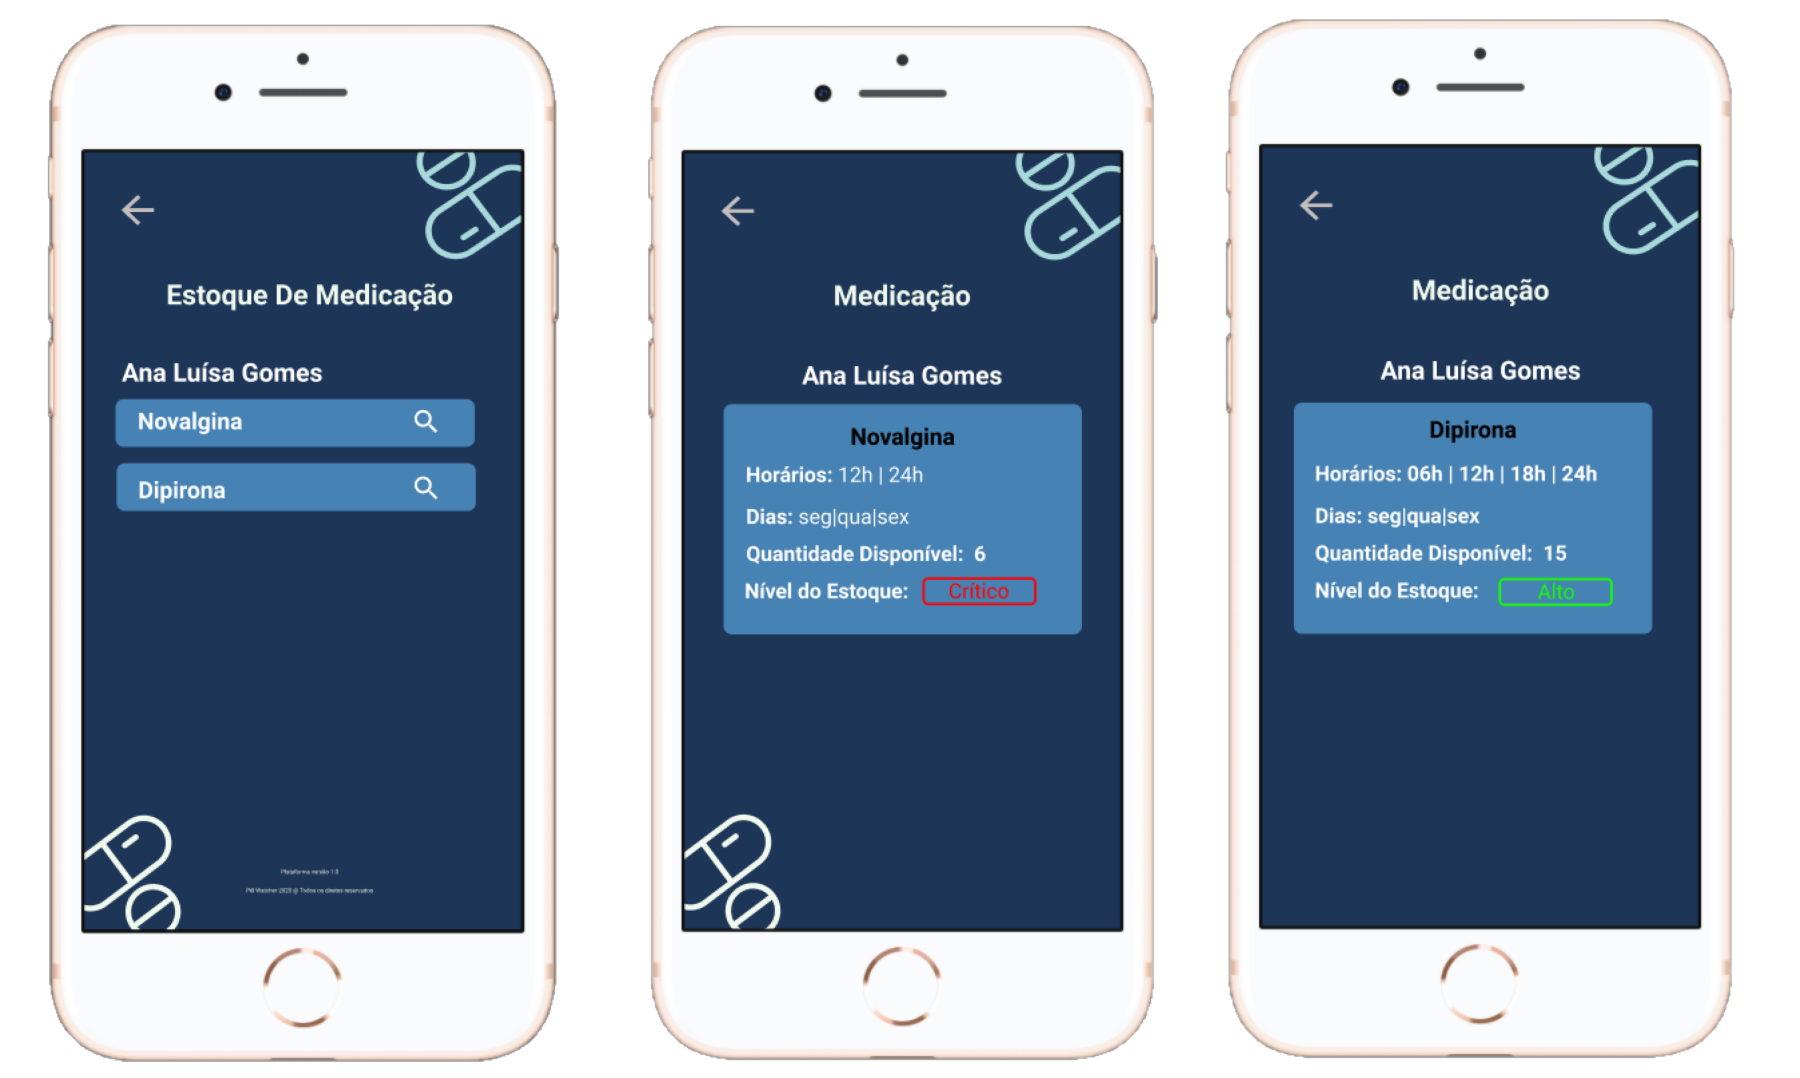
\includegraphics[width=15cm]{figuras/software/Atual_prototipo/Paciente_estoqueDeMedicacao.png}
    \caption{Paciente - Fluxo para visualizar o estoque de medicação}
    \label{fig:prototipo_paciente_estoqueDeMedicacao}
\end{figure}

\begin{table}[H]
    \centering
    \caption{Tabela de interações das telas de estoque de medicação}
    \label{tab:interacao-telas-notificacao_estoqueDeMedicacao}
    \begin{adjustbox}{max width = \textwidth}
    % \begin{adjustwidth}{-2,5cm}{}
        \begin{tabular}{|L{5cm}|L{6cm}|L{4cm}|L{4cm}|L{4cm}|}
            \hline
            \rowcolor[HTML]{A8DADC}
            \multicolumn{1}{|c|}{\textbf{Tela}} & \multicolumn{1}{c|}{\textbf{Entrada}} & \multicolumn{1}{c|}{\textbf{Interações}} & \multicolumn{1}{c|}{\textbf{Saída}} & \multicolumn{1}{c|}{\textbf{Alternativo}} \\ \hline
             Tela inicial de estoque de medicação & Botão `Estoque de medicação' do menu inicial do paciente  & Visualizar as medicações e seus respectivos dados & Botão `Visualizar' de uma medicação  & Botão 'Voltar' que irá direcionar para o menu inicial do paciente  \\ \hline
             Tela de visualizar estoque de uma medicação & Botão `Visualizar' da medicação selecionada na tela inicial de estoque de medicação & Visualizar dados do estoque da medicação selecionada & Botão `Voltar' que irá direcionar para tela inicial de estoque de medicação do paciente  & \multicolumn{1}{c|}{---} \\ \hline
        \end{tabular}
    % \end{adjustwidth}
    \end{adjustbox}
\end{table}

% \subsubsubsection{Relatório de medicação}
\subparagraph*{} $-$ Relatório de medicação

A Fig. \ref{fig:prototipo_paciente_relatorioDeMedicacao} indica o fluxo para visualizar os relatórios de medicação semanais disponíveis do paciente que trazem informações como data, medicação, enfermeiro e status da entrega.

\begin{figure}[H]
    \centering
    \includegraphics[width=12cm]{figuras/software/Atual_prototipo/Paciente_relatorioDeMedicacao.png}
    \caption{Paciente - Fluxo para visualizar o relatório de medicação}
    \label{fig:prototipo_paciente_relatorioDeMedicacao}
\end{figure}

\begin{table}[H]
    \centering
    \caption{Tabela de interações das telas de relatório de medicação}
    \label{tab:interacao-telas-notificacao_relatorioDeMedicacao}
    \begin{adjustbox}{max width = \textwidth}
    % \begin{adjustwidth}{-2,5cm}{}
        \begin{tabular}{|L{5cm}|L{6cm}|L{4cm}|L{4cm}|L{4cm}|}
            \hline
            \rowcolor[HTML]{A8DADC}
            \multicolumn{1}{|c|}{\textbf{Tela}} & \multicolumn{1}{c|}{\textbf{Entrada}} & \multicolumn{1}{c|}{\textbf{Interações}} & \multicolumn{1}{c|}{\textbf{Saída}} & \multicolumn{1}{c|}{\textbf{Alternativo}} \\ \hline
             Tela inicial do relatório de medicação & Botão `Relatório de Medicação' do menu inicial do paciente & Visualizar relatórios semanais disponíveis & Botão `Visualizar' do relatório selecionado  & Botão `Voltar' que irá direcionar para o menu inicial do paciente  \\ \hline
             Tela de relatório de medicação & Botão `Visualizar' do relatório selecionado & Visualizar informações das medicações ministradas na semana de vigência do relatório & Botão `Voltar' que irá direcionar para a tela inicial do relatório de medicação & \multicolumn{1}{c|}{---} \\ \hline
        \end{tabular}
    % \end{adjustwidth}
    \end{adjustbox}
\end{table}

\section{Inovação no Software}
\subsection {\textit{IoT - Internet of Things}}
\textit{Internet of Things} é a interconexão de objetos com a internet. No projeto \emph{PillWatcher}, o dispensador de medicamentos irá se comunicar com o aplicativo por meio de um \textit{Broker} MQTT, que é como uma espécie de mediador entre as máquinas, capaz de fazer com que a comunicação de fato ocorra entre elas. O \textit{Broker} utilizado será o \textit{Mosquitto}.

O protocolo MQTT é um dos mais utilizados na indústria para a implementação de automações e de tecnologias como a IoT – internet das coisas. Sigla para \textit{Message Queuing Telemetry Transporte}, ele pode ser resumido como uma forma de realizar a comunicação entre as máquinas.\cite{ENGPROCESS_2018}

E o \textit{Mosquitto} nada mais é do que um dos componentes do protocolos MQTT. Cada vez mais usado no setor industrial, ele aparece como uma forma de otimizar o tempo e tornar os processos mais simples \cite{ENGPROCESS_2018}.

\subsection {Arquitetura de Microsserviços}
A arquitetura de microsserviços permite a entrega e implantação contínua de aplicações grandes e complexas. Além disso, há a melhoria na manutenção, onde cada serviço é relativamente pequeno e, portanto, mais fácil de entender e mudar. Traz consigo também uma melhor testabilidade, devido ao fato de que os serviços são menores e mais rápidos de testar. A implantabilidade dos serviços podem ser feitas de forma independente e permite que a organização do esforço de desenvolvimento em torno de várias equipes seja autônoma.

A arquitetura do \textit{Pillwatcher} foi planejada e construída com base nesse conceito. Assim, serão confeccionadas três \textit{APIs}: administrador, enfermeiro e paciente. Tais \textit{APIs} tratam de aspectos relacionados a esses e uma \textit{API Gateway} para centralizar e gerenciar as chamadas dos microsserviços citados.

\subsection {\textit{Reactive Programming}}
A programação reativa é um paradigma de programação assíncrona, preocupado com fluxos de dados e a propagação de mudanças. Isso significa que é possível expressar fluxos de dados estáticos (por exemplo, matrizes) ou dinâmicos (por exemplo, emissores de eventos com facilidade por meio da  linguagem  de programação empregada).

Partindo do pressuposto que o \textit{Pillwatcher} seria utilizado em larga escala, a quantidade de requisições também estaria nessas proporções e se realizadas de forma síncrona, ou seja, cada requisição espera a resposta para continuar seu processamento, o resultado acerca do tempo de resposta não seria viável, dessa forma, serão utilizadas requisições assíncronas. Por isso, faz-se necessário incorporar o paradigma apresentado no parágrafo anterior na solução visando melhorar a experiência do usuário e facilitar a implementação por parte dos desenvolvedores.